\documentclass[IWBstudentthesis%     style
              ,optCharter%           font
              %,optCMYK%             color model
              ,optBibtex% 	         bibliography tool
              ,optBibstyleNumeric   %lbam (ieee) citation style
              ,optEnglish% 		 language
              ,optCenterEquations%
              %,optTikzExternalize%  compiles faster for large tikz images
              ]{IWBlatex}%
%
% Set paths

\usepackage{chngcntr}
\usepackage{microtype}
\usepackage{graphicx}
\usepackage{subcaption}
\usepackage{verbatim}
\usepackage{textcomp}
% define math operator
\usepackage{amsmath}
\DeclareMathOperator{\sigmoid}{sigmoid}
%
\graphicspath{{figures/}}%
\addbibresource{literature/literature.bib}%
\makenoidxglossaries%
%A--------------------------------------------------------
\newacronym{am}{AM}{Additive Manufacturing}%
%C--------------------------------------------------------
\newacronym{cad}{CAD}{Computer Aided Design}%
%I--------------------------------------------------------
\newacronym{ir}{IR}{infrared}%
\newacronym{iwb}{\textit{iwb}}{Institut für Werkzeugmaschinen und Betriebswissenschaften}%
%L--------------------------------------------------------
\newacronym{lbam}{LBAM}{Professorship Laser-based Additive Manufacturing}%
%M--------------------------------------------------------
\newacronym{ml}{ML}{Machine Learning}%
\newacronym{msi}{MSI}{Multispectral Imaging}
%P--------------------------------------------------------
\newacronym{pbf}{PBF}{Powder Bed Fusion}%
\newacronym{pbflb}{PBF-LB}{Laser-based Powder Bed Fusion}%
\newacronym{pbflbm}{PBF-LB/M}{Laser-based Powder Bed Fusion of Metals}
\newacronym{pbflbp}{PBF-LB/P}{Laser-based Powder Bed Fusion of Polymers}%
%R--------------------------------------------------------
\newacronym{ros}{ROS}{Robot Operating System}%
\newacronym[\glslongpluralkey={Arbeitspakete}]{ap}{AP}{Arbeitspaket}%
%s--------------------------------------------------------
\newacronym{sls}{SLS}{Selective Laser Sintering}%%
\newglossaryentry{latex}%
{%
	name=Latex,%
	description={Generische Mark-up-Sprache zum Erstellen wissenschaftlicher Texte. Sie ist in jeder Hinsicht Word überlegen, welches einem visuellen Mark-Up entspricht. Das X von \LaTeX\ wird als ç (Stimmloser palataler Frikativ) ausgesprochen, vergleiche deutsche Aussprache von \textit{ch}.}%
}%
\newglossaryentry{tutorial}%
{%
	name=Tutorial,%
	description={Kurze Gebrauchsanleitung welche ein Thema, einen gewissen Vorgang oder eine Funktion erklärt. Hat nicht den Anspruch auf Vollständigkeit.}%
}%
\newglossaryentry{tikz}%
{%
	name=Ti\textit{k}Z,%
	description={Frontend-Paket, das auf PGF-Plot aufbaut und zum Erstellen von Graphiken dient.}%
}%%
% Custom macros
% Einheitliche Schreibweise
% ---------------------------------------
\newcommand{\zb}{z.\,B.\xspace}%
\renewcommand{\dh}{d.\,h.\xspace}%
\newcommand{\uu}{u.\,U.\xspace}%
\newcommand{\ua}{u.\,a.\xspace}%
\newcommand{\idr}{i.\,d.\,R.\xspace}%
\newcommand{\vgl}{vgl.\xspace}%
\newcommand{\sa}{s.\,a.\xspace}%
\newcommand{\bzw}{bzw.\xspace}%
\newcommand{\evtl}{evtl.\xspace}%
\newcommand*{\eg}{e.\,g.\xspace}%
\newcommand*{\ie}{i.\,e.\xspace}%
% Leichtere Zitate
% ---------------------------------------
% \cite{} gut für Shorthand (Normen) im Text --> alternative zu \textcite
\newcommand{\autor}[2]{\textcite[#1]{#2}}%
\newcommand{\zitat}[2]{\parencite[#1]{#2}}%
\newcommand{\zitatpre}[3]{\parencite[#1][#2]{#3}}%
\newcommand{\zitate}[4]{\parencites[#1]{#2}[#3]{#4}}%
\newcommand{\zitatee}[6]{\parencites[#1]{#2}[#3]{#4}[#5]{#6}}%
\newcommand{\zitateee}[8]{\parencites[#1]{#2}[#3]{#4}[#5]{#6}[#7]{#8}}%
% ---------------------------------------
\newcommand{\insertref}{\todo[color=green!40]{Missing ref}}%
% Leichtere Bilder
% ---------------------------------------
\newcommand{\bild}[4]{%
	\begin{figure}[#1]
		\centering
		\includegraphics
		[
		width=#2\textwidth,
		]
		{figures/#3}
		
		\caption{#4}
		\label{fig:#3}
	\end{figure}
}
%
%
\newcommand{\bildsvg}[4]{
	\begin{figure}[#1]
		\centering%
		\def\svgwidth{#2\columnwidth}%
		\input{figures/#3}%
		%
		\caption{#4}%
		\label{fig:#3}%
	\end{figure}	
}
%
\newcommand{\bildtikz}[4]{
	\begin{figure}[#1]
		\centering
		\scalebox{#2}{\input{figures/#3}}
		\caption{#4}
		\label{fig:#3}
	\end{figure}
}
%
\newcommand{\bildtikzvar}[5]{
	\begin{figure}[#1]
		\centering
		\scalebox{#2}{\input{figures/#3}}
		\caption{\parbox[t]{#4\textwidth}{#5}}
		\label{fig:#3}
	\end{figure}
}
%
\newcommand{\bildtrim}[5]{% Mit definiertem Beschnitt
	\begin{figure}[#1]
		\centering
		\includegraphics
		[
		width=#2\textwidth,
		%keepaspectratio=true,
		trim=#3,		% l u r o
		clip,
		]
		{figures/#4}
		
		\caption[]{#5}
		\label{fig:#4}
	\end{figure}
}
%
\newcommand{\bildvar}[5]{% Mit definierter Breite / Zeilenumbruch der Caption
	\begin{figure}[#1]
		\centering
		\includegraphics
		[
		width=#2\textwidth,
		]
		{figures/#3}
		
		\caption[]{\parbox[t]{#4\textwidth}{#5}}
		\label{fig:#3}
	\end{figure}
}
%
\newcommand{\bildbox}[4]{% Bild mit Rahmen
	\begin{figure}[#1]
		\centering
		\fbox{%
			\includegraphics
			[
			width=#2\textwidth,
			]
			{figures/#3}
		}
		\caption[]{#4}
		\label{fig:#3}
	\end{figure}
}
%
\newcommand{\bildboxtrim}[5]{%
	\begin{figure}[#1]
		\centering
		\fbox{%
			\includegraphics
			[
			width=#2\textwidth,
			%keepaspectratio=true,
			trim=#3,		% l u r o
			clip,
			]
			{figures/#4}
		}
		\caption[]{#5}
		\label{fig:#4}
	\end{figure}
}
%
\newcommand{\bildboxvar}[5]{%
	\begin{figure}[#1]
		\centering
		\fbox{%
			\includegraphics
			[
			width=#2\textwidth,
			]
			{figures/#3}
		}
		\caption[]{\parbox[t]{#4\textwidth}{#5}}
		\label{fig:#3}
	\end{figure}
}
%
\newcommand{\bildsvgvar}[5]{
	\begin{figure}[#1]
		\centering
		\def\svgwidth{#2\columnwidth} 
		\subimport*{figures/}{#3}
		\caption{\parbox[t]{#4\textwidth}{#5}}
		\label{fig:#3}
	\end{figure}	
}
%
\newcommand{\bildpdf}[3]{%
	\begin{figure}[H]
		\centering
		\includegraphics
		[
		width=#1\textwidth,
		page={#2},
		]
		{#3}
		%\caption[]{#4}
		\label{fig:#3}
	\end{figure}
}
% ---------------------------------------%

% set up list of figures
\usepackage[titles]{tocloft}
\newlength{\mylen}
\renewcommand{\cftfigpresnum}{\figurename\enspace}
\settowidth{\mylen}{\cftfigpresnum\cftfigaftersnum}

\addtolength{\cftfignumwidth}{\mylen}
%
\sloppy
% Extra packages for LBAM formatting-------------------------------------------
% continous figure and table counter (arabic numbers Fig 1., Fig 2. etc. not Fig. 1.1, Fig 1.1)

\counterwithout{figure}{chapter}%
\counterwithout{table}{chapter}%
%--------------------------------------
\begin{document}%
\hyphenpenalty=5000
\tolerance=1000
% Titlepage
% ---------
\frontmatter%
% Info: replace Prof Reinhart by Prof. Zäh:\IWBnamesProfZaeh \newline \IWBlangChairMWIWBLWF
% Info: separate multiple supervisors by \newline
% \IWBstudentthesisTitlePageCustomMastersThesis{Untersuchung des multispektralen
% Bildgebungsverfahrens zur Temperaturbestimmung auf einer numerischen
% Experimentierplattform beim Laser-basierten Pulverbett-Schmelzverfahren
% von Metallen.}
% {Investigation of multispectral imaging algorithm for temperature
% determination on a numerical experiment platform in Laser-based 
% Powder Bed fusion of Metals}
% {Zhaoyong Wang \newline Connollystr.3 \newline 80809 München}
% {\IWBnamesProfWudy \newline M.Sc. Ruihang Dai \newline \IWBlangChairMWLBAM}
% {\IWButilsDate{31}{07}{2023}}%
%
% 
% \node[options] (id) at position {label};
% \IWBstudentthesisTitlePageCustomBachelorsThesis{German Title}{English Title}{Martin Mustermann \newline Musterweg 20 \newline 80999 München}{\IWBnamesProfReinhart \newline \IWBlangChairMWIWBLBM}{\IWButilsDate{1}{1}{2018}}%
\IWBstudentthesisTitlePageCustomSemesterThesis{Untersuchung des multispektralen
Bildgebungsverfahrens zur Temperaturbestimmung auf einer numerischen
Experimentierplattform beim Laser-basierten Pulverbett-Schmelzverfahren
von Metallen.}
{Investigation of multispectral imaging algorithm for temperature
determination on a numerical experiment platform in Laser-based 
Powder Bed fusion of Metals}
{Zhaoyong Wang \newline Connollystr.3 \newline 80809 München}
{\IWBnamesProfWudy \newline M.Sc. Ruihang Dai \newline \IWBlangChairMWLBAM}
{\IWButilsDate{31}{07}{2023}}%
%
%\IWBstudentthesisTitlePageCDIDP{German Title}{English Title}{Martin Mustermann \newline Musterweg 20 \newline 80999 München}{\IWBnamesProfReinhart \newline \IWBlangChairMWIWBLBM}{\IWButilsDate{1}{1}{2018}}%
%
% Task formulation
% ----------------
% Deckblatt
\chapter*{Scope of Work}

%\markright{Aufgabenstellung} 	% Kolumnentitel manuell auf "Aufgabenstellung"

\textbf{Title of the Master's Thesis:}\\
\Large{Manually Change you Thesis Title here}\\
%\newline
%\normalsize{\textbf{(English Title of the Bachelor's/Master's Thesis/Semester Thesis/In\-ter\-dis\-ci\-pli\-na\-ry Project:)}}\\
%\Large{Development...}
\normalsize

\begin{tabbing}
	\hspace{7em} 		\= \hspace{13em}			\= \hspace{7em} 		\= \kill
	\textbf{Author:}  \> B.Sc. Max Mustermann 	\> \textbf{Supervisor:} 	\>  M.Sc. Mein Betreuer \\
	\textbf{Issuance:} 	\> 01.07.2021 	\> \textbf{Submission:} 	\> 31.12.2021
\end{tabbing}

\vspace{5mm}
\textbf{Setting:}\\
\blindtext%

\vspace{5mm}
\textbf{Objective:}\\
\blindtext

\vspace{5mm}
\textbf{Methodology:} \\
The content of the present thesis can be subdivided into the following tasks
\begin{itemize}
	\item Method 1
	\item Method 2
	\item Method 3
	\item etc.
\end{itemize}
\vspace{1.0cm}

\chapter*{Declaration}
I hereby confirm that this master's/ bachelor's/ semester thesis was written independently by myself without the use of any sources beyond those cited, and all passages and ideas taken from other sources are cited accordingly.%
%
\vspace{5cm}\\
\begin{tabular}{p{0.5\linewidth}p{0.5\linewidth} }
	.....................................................		& .....................................................\\
	Location, Date  	& Signature
\end{tabular}
%
\vspace{2cm}\\
%
With the supervision of Mr. Max Mustermann by Mr. Mein Betreuer intellectual property of the \gls{lbam}  flows into this work. A publication of the work or a passing on to third parties requires the permission of the head of the professorship. I agree to the archiving of the printed thesis in the  \gls{lbam} library (which is only accessible to \gls{lbam} staff) and in \gls{lbam}'s digital thesis database as a PDF document.%
%
\vfill
%
\begin{tabular}{p{0.5\linewidth}p{0.5\linewidth} }
	.....................................................		& .....................................................\\
    Location, Date  	& Signature
\end{tabular}
%
%
% Abstract
% --------
% In total max. 1 Page!
\IWBstudentthesisAbstract{%
	%
	% Abstract English:
	Temperature is one of the most important parameters in \gls{pbflbm}. 
	so, monitoring the temperature at melt pool necessary. It is still challenging to get 
	multispectral image without interference.
	In oder to achieve this, a numerical experiment platform is formed.
	Within this virtual experimentation platform, a virtual multispectral camera has been 
	incorporated, taking into account the operational principles of actual sensors. 
	In this multispectral camera, the digital values are computed through the integration 
	of radiance intensity over wavelength. Then, hypothetical material models have been 
	developed based on various sets of raw emissivity data. Within these hypothetical material 
	models, emissivity values are configured to be wavelength and temperature-dependent, 
	effectively simulating the phase transition phenomena observed in real materials. 
	This approach enables the emulation of emissivity characteristics akin to those found in 
	actual materials. Lastly, based on the generated experimental data, a temperature 
	estimation algorithm has been developed. This algorithm is capable of simultaneously 
	estimating the temperature and emissivity of the material using the experimental data. 
	By comparing and analyzing different temperature estimation algorithms, the importance 
	of emissivity model selection within the temperature estimation algorithm has been demonstrated. 
	Through calculations involving materials within various temperature ranges, the 
	applicability of the temperature estimation algorithm has been established.
	\newpage
}{%
	%
	% Zusammenfassung Deutsch
	Temperatur ist einer der wichtigsten Parameter im \gls{pbflbm}. Daher ist die Überwachung der 
	Temperatur am Melt-pool notwendig. Es bleibt jedoch eine Herausforderung, multispektrale 
	Bilder ohne Störungen zu erhalten. Um dies zu erreichen, wurde eine numerische 
	Experimentierplattform entwickelt. Innerhalb dieser virtuellen Experimentierplattform 
	wurde eine virtuelle Multispektralkamera integriert, unter Berücksichtigung der 
	Funktionsprinzipien tatsächlicher Sensoren. In dieser Multispektralkamera werden die 
	digitalen Werte durch die Integration der Strahlungsintensität über die Wellenlänge 
	berechnet. Anschließend wurden hypothetische Materialmodelle basierend auf verschiedenen 
	Sätzen von rohen Emissionsdaten entwickelt. Innerhalb dieser hypothetischen Materialmodelle 
	werden Emissionswerte konfiguriert, die wellenlängen- und temperaturabhängig sind und 
	somit Phasenübergangsphänomene simulieren, wie sie in realen Materialien beobachtet werden. 
	Dieser Ansatz ermöglicht die Simulation von Emissionscharakteristika, ähnlich denen in 
	tatsächlichen Materialien. Schließlich wurde basierend auf den generierten experimentellen 
	Daten ein Temperaturschätzalgorithmus entwickelt. Dieser Algorithmus ist in der Lage, 
	die Temperatur und Emissivität des Materials gleichzeitig unter Verwendung der 
	experimentellen Daten abzuschätzen. Durch den Vergleich und die Analyse 
	verschiedener Temperaturschätzalgorithmen wurde die Bedeutung der Auswahl 
	des Emissionsmodells innerhalb des Temperaturschätzalgorithmus demonstriert. 
	Durch Berechnungen von Materialien in verschiedenen Temperaturbereichen wurde die 
	Anwendbarkeit des Temperaturschätzalgorithmus festgestellt.%
	\thispagestyle{empty}
}%
%
%%
%
% Content
% -------
\IWBstudentthesisPrintTableOfContents%
% \tableofcontents
%
% List of Abbreviations --> for LBAM moved to end document
% ---------------------
%\printnoidxglossary[type=acronym,sort=standard,title={\IWBlangAcronyms}]
%
% Mainmatter
% ----------
\mainmatter%
% !TeX spellcheck = de_DE
\chapter{LaTeX-Tutorial}%
Dieses \gls{tutorial} liefert eine Kurzeinführung in die Verwendung von \gls{latex}.%
%
\section{Titelseite}%
Die Titelseite wird in {./main.tex} definiert. Der Studienarbeitstyp wird durch Ein- und Auskommentieren der Befehle%
\begin{itemize}%
	\item \verb|\IWBstudentthesisTitlePageCustomMastersThesis|,%
	\item \verb|\IWBstudentthesisTitlePageCustomBachelorsThesis| und%
	\item \verb|\IWBstudentthesisTitlePageCustomSemesterThesis|%
\end{itemize}%
ausgewählt und die Seite entsprechend der Argumente gesetzt. Die Professoren und Lehrstuhle können mittels der Makros%
\begin{itemize}%
	\item \verb|\IWBnamesProfReinhart \newline \IWBlangChairMWIWBLBM| oder%
	\item \verb|\IWBnamesProfZaeh \newline \IWBlangChairMWIWBLWF|%
\end{itemize}%
ausgewählt werden.%
%
\section{Zitation}%
%
Zum Zitieren stehen die Standartbefehle \verb|\textcite| und \verb|\parencite| zur Verfügung. Soll der Autorename im Satz verwendet werden, eignet sich ersteres, z.B. \textcite[2-3]{Bayerlein2018} bezieht sich auf \textcite{Bayerlein2016469}. Soll das Zitat in Klammern nach die Aussage gestellt werden empfiehlt sich zweiteres \parencite{Zaeh2018385}. Sammelzitationen am Satzende schreiben sich wie folgt \parencite{Kleinwort2018658,Kleinwort20189,Kleinwort2018631}. Die Zitation von Online-Quellen kann schwierig sein, da nicht immer der Autor und das Erscheinungsjahr verfügbar sind. Vergleicht man \textcite{Heuss2018} und \textcite{iwb-Startseite}, stellt man fest, dass bei zweiteren der Seitentitel statt des bekannten Schemas eingesetzt wird.\par%
%
Normen werden als \textcite{ISO.10218-2} dargestellt. Im Bibtex-Export des verwendeten Literaturverwaltungsprogramm sind bestimmte Einstellungen vorzunehmen. Dokumententyp ist \enquote{@book} mit folgenden Einträgen:
\begin{itemize}
	\item Normtyp und Nummer als \enquote{title}
	\item Langtitel als \enquote{subtitle}
	\item Verlag als \enquote{publisher}
	\item Jahr als \enquote{date}
	\item \enquote{author} darf nicht belegt werden!
\end{itemize}
%
\section{Abkürzungen}
In {./source/abbreviations.tex} können Abkürzungen definiert werden. Es gibt Besonderheiten zu Ausdrücken, deren Pluralendung nicht auf s endet. Hier müssen ggf. Kurz- und Langformen des Ausdrucks auch für den Plural definiert werden.\par%
\begin{itemize}
	\item \verb|\gls{ros}|: schreibt beim ersten Auftreten im Dokument ausführlich \gls{ros}, ab dem zweiten Auftreten wird abgekürzt \gls{ros}% 
	\item \verb|\glspl{ap}| verwendet den Plural in Langform \glspl{ap} und danach in Kurzform \glspl{ap}%
\end{itemize}%
%
\section{Glossar}
In {./source/glossary.tex} können Begriffe erklärt, abgegrenzt oder definiert werden. Begriffe erhalten einen Namen und eine Beschreibung als Glossareintrag sowie ein Lable zum Referenzieren im Text. Ein Glossar ist Optional.\par%
\begin{itemize}%
	\item \verb|\gls{latex}|: Schreibt den Namen aus dem Glossarverzeichnis mit Verweis auf den Glossareintrag \gls{latex}%
\end{itemize}%
%
\section{Abbildungen}
Graphiken und Bilder können in beliebigen Dateiformaten eingebunden werden, vergleiche \cref{fig:MyImage}. Vektorgraphiken sind im Allgemeinen Pixelgraphiken in Schärfe und Speicherbedarf überlegen.\par%
%
\begin{figure}[htb]%
    \centering%
    %
    % Including .png
    
\includegraphics[width=40mm]{figures/ImagePNG.png}%
    %
    \hspace*{5mm}%
    %
    % Including .pdf
    
\includegraphics[width=40mm]{figures/ImagePDF.pdf}\par%
    %
    % Including .tikz
    \begingroup%
        %\AMtikzExternalizeSkipNext%
        \resizebox{40mm}{!}{\begin{tikzpicture}[inner sep=0pt, outer sep=0pt]%
    \fill [draw=TUMBlue,line width=5mm,fill=none] (0mm,0mm) rectangle (95mm,95mm);%
    \node at (50mm,50mm) {\fontsize{60}{60}\selectfont TIKZ};%
\end{tikzpicture}%
}%
    \endgroup%
    %
    \hspace*{5mm}%
    %
    % Including .pdf_tex
    \begingroup%
        \def\svgwidth{40mm}%
        \fontsize{25}{25}\selectfont%
        \input{figures/ImagePDFTEX.pdf_tex}%
    \endgroup%
    %
    \caption{Beschreibung des Bilds. Außerdem machen wir nun die Bildunterschrift unnötig lang um die Formatierung zu testen. \label{fig:MyImage}}%
\end{figure}%
%
\begin{figure}[htb]%
    \centering%
    \small%
\pgfplotstableread{figures/datatable2d.dat}{\datatableTwoDim}%
\begin{tikzpicture}[scale=1]%
    \begin{axis}[width = 9cm, height = 6cm, scale only axis=true%
                 ,xmin = 0%
                 ,xmax = 10%
                 ,xlabel = {$t$ in s}%
                 ,xtick distance = 1%
                 ,ymin = -1.2%
                 ,ymax = 1.2%
                 ,ylabel = {y-Label}%
                 ,ytick distance = 0.5%
                 ,grid = both%
                 ,grid style = {line width = .1pt, draw = TUMBlack!10}%
                 ,legend style = {at = {(0.1cm,0.1cm)}, anchor = south west,font=\small}%
                 ,\IWBlangGerEng{/pgf/number format/use comma}{}%
                 ]%
        \addplot [TUMBlue,very thick] table [x={X}, y={Y1}] {\datatableTwoDim};%
        \addplot [TUMBlue3,very thick,dashed] table [x={X}, y={Y2}] {\datatableTwoDim};%
        \addplot [TUMBlack,very thick,dotted] table [x={X}, y={Y3}] {\datatableTwoDim};%
        \legend{$\sin(t)$,$\cos(t)$,$0.5$};%
    \end{axis}%
\end{tikzpicture}%
%
%
%
    \caption{Beschreibung des Plots. Außerdem machen wir nun die Bildunterschrift unnötig lang um die Formatierung zu testen. \label{fig:PlotTwoDim}}%
\end{figure}%
%
Für Nutzer mit perfektionistischen Anspruch empfiehlt sich die Nutzung von \gls{tikz}. Vorteil ist, dass die Erzeugung von Daten und die Darstellung komplett getrennt werden. Die Darstellung erfolgt einheitlich gemäß eines generischen Mark-Ups, vergleiche \cref{fig:PlotTwoDim,fig:PlotThreeDim}.\par%
%
\vspace{12pt}%
\begin{figure}[htb]%
    \centering%
    \small%
\pgfplotsset{colormap={mycolormap}{rgb255=(255,255,0) rgb255=(255,0,0)}}%    
\begin{tikzpicture}%
    \begin{axis}[width = 10cm, height = 8cm%
                ,xmin = -1%
                ,xmax = 1%
                ,xlabel = {$x$ in m}%
                ,xtick distance = 0.5%
                ,ymin = -1%
                ,ymax = 1%
                ,ylabel = {$y$ in m}%
                ,ytick distance = 0.5%
                ,zmin = 0%
                ,zmax = 1%
                ,zlabel = {$z$ in m}%
                ,ztick distance = 0.2%
                ,grid = both%
                ,grid style = {line width = .1pt, draw = TUMBlack!10}%
                ,colorbar%
                ,view={60}{30}%
                ,\IWBlangGerEng{/pgf/number format/use comma}{}%
                ]%
        \addplot3 [surf,z buffer=sort] table[x={X}, y={Y}, z={Z}] {figures/latex_tutorial/datatable3d.dat};%
    \end{axis}%
\end{tikzpicture}%
%
%
%
    \caption{Beschreibung des Plots. Außerdem machen wir nun die Bildunterschrift unnötig lang um die Formatierung zu testen. \label{fig:PlotThreeDim}}%
\end{figure}%
%
%
%
% !TeX spellcheck = en_US
\glsresetall%
\chapter{Introduction}%
%\gls{am} is the umbrella term for a variety of technologies, describing the automated process of manufacturing physical parts directly from virtual \gls{cad} models. %
%\gls{pbflbp}, also known as \gls{sls}, as part of the \gls{am} process group
\blindtext%
%
%
\section{Section Introduction}%
\blindtext%
%
%
\subsection{Subsection Introduction}%
\blindtext%
%
%
\section{Another Section Introduction}%
\blindtext%
%
%
\section{Many Section Introductions}%
\blindtext%
%
%
\section{Many More Section Introductions}%
\blindtext%
Another lorem ipsum to test formatting. \\%
\blindtext%
And one more for good measure.\\%
\blindtext%
Rinse and repeat. \\%
\blindtext[3]%
\section{Testing the Continuous Figure Numbering}%
Here we have a graph which should have a continuous caption numbering \ie it should say Figure 4 or Figure 5, instead of Figure 2.1 or Figure 2.2.
\begin{figure}[htb]%
	\centering%
	\small%
\pgfplotsset{colormap={mycolormap}{rgb255=(255,255,0) rgb255=(255,0,0)}}%    
\begin{tikzpicture}%
    \begin{axis}[width = 10cm, height = 8cm%
                ,xmin = -1%
                ,xmax = 1%
                ,xlabel = {$x$ in m}%
                ,xtick distance = 0.5%
                ,ymin = -1%
                ,ymax = 1%
                ,ylabel = {$y$ in m}%
                ,ytick distance = 0.5%
                ,zmin = 0%
                ,zmax = 1%
                ,zlabel = {$z$ in m}%
                ,ztick distance = 0.2%
                ,grid = both%
                ,grid style = {line width = .1pt, draw = TUMBlack!10}%
                ,colorbar%
                ,view={60}{30}%
                ,\IWBlangGerEng{/pgf/number format/use comma}{}%
                ]%
        \addplot3 [surf,z buffer=sort] table[x={X}, y={Y}, z={Z}] {figures/latex_tutorial/datatable3d.dat};%
    \end{axis}%
\end{tikzpicture}%
%
%
%
	\caption{Beschreibung des Plots. Außerdem machen wir nun die Bildunterschrift unnötig lang um die Formatierung zu testen. \label{fig:PlotThreeDimTEst}}%
\end{figure}%
%
%
\section{Now Let's test tables}%
The \cref{table:TestTableCaption} should have captions above the table instead of captions below, like Figures. \\%
%
\begin{table}[h!]%
	\centering%
	\caption{This table caption should be above the table. Otherwise DIN is going to judge you...}%
	\begin{tabular}{||c c c c||}%
		\hline%
		Col1 & Col2 & Col2 & Col3 \\ [0.5ex]% 
		\hline\hline%
		1 & 6 & 87837 & 787 \\% 
		2 & 7 & 78 & 5415 \\%
		3 & 545 & 778 & 7507 \\%
		4 & 545 & 18744 & 7560 \\%
		5 & 88 & 788 & 6344 \\ [1ex]% 
		\hline%
	\end{tabular}%
	\label{table:TestTableCaption}%
\end{table}%
%
%
%
% !TeX spellcheck = en_US
\chapter{State of the art}%
\gls{am} has undergone significant advancement since its inception 25 years 
ago\cite{J.Scott.2012}. Presently, \gls{am} has achieved widespread 
utilization across industries including aerospace and dentistry. 
It demonstrates versatile capabilities for processing materials 
like metals, ceramics, polymers as well as composites\cite{Frazier.2014}.
Many researchers have classified these processing techniques into the following 
categories\cite{Kruth.1991,Hartke.2011}:

\begin{itemize}
    \item \gls{vpp}
    \item \gls{mjt}
    \item \gls{bjt}
    \item \gls{mex}
    \item \gls{pbf}
    \item \gls{shl}
    \item \gls{ded}
\end{itemize}

Each process possesses its own advantages and disadvantages, 
contingent upon factors such as the materials being processed, 
construction speed, dimensional accuracy, etc\cite{Hartke.2011}.


In this work, the primary focus is the monitoring process in \gls{pbflbm}.
Hence, in this chapter, the \gls{pbflbm} technology will be
introduced, followed by an exploration of the monitoring methods employed 
in contemporary \gls{pbflbm}. Among these methods, multispectral imaging 
has been selected as the monitoring technique utilized in this work. 
Consequently, this establishes the underlying principles of the 
observation aspect within \gls{pbflbm}. Subsequently, the material's 
emissivity model will be introduced, thus leading to the current 
temperature estimation algorithms in use.
%
%
\section{Laser-based Powder Bed Fusion of Metals}
In 1989, Carl Deckard and Joe Beaman pioneered a technique 
\gls{sls}. Within this methodology, high-energy density lasers are 
focused onto the surface of metal powder, resulting in the formation of 
a solidified metal layer\cite{Mazzoli.2013,Wong.2012}. 
In the year 2002, Fisher et al. observed a phenomenon of partial melting 
in metal powders. This discovery led to the potential reduction of porosity 
in components produced through the original \gls{sls} process, subsequently 
enhancing the mechanical properties of the materials. However, it should be 
noted that complete elimination of porosity remains unattainable within the 
partial melting sintering methodolgy\cite{Fischer.2002}.


With the development of laser technology, the utilization of partial 
melting in \gls{sls} has been supplanted by the \gls{slm} approach. 
Within this technique, metal powder is subjected to complete melting, 
resulting in an elevated density of the produced part. However, 
the heightened thermal gradient inherent in this method gives rise to 
internal stresses within the finalized components\cite{Hooper.2018}, necessitating
heat treatment to alleviate these effects\cite{Osakada.2006}.


\gls{pbflb} is a type of \gls{am} process that uses a 
laser beam to selectively melt and fuse metal powder layers according 
to a digital model\cite{Swift.2013}, which includes \gls{sls} and \gls{slm}.
The structure of the \gls{pbflbm} machine can be found in Fig.\ref{fig: pbflbm}.

\begin{figure}[htbp]
    \centering
    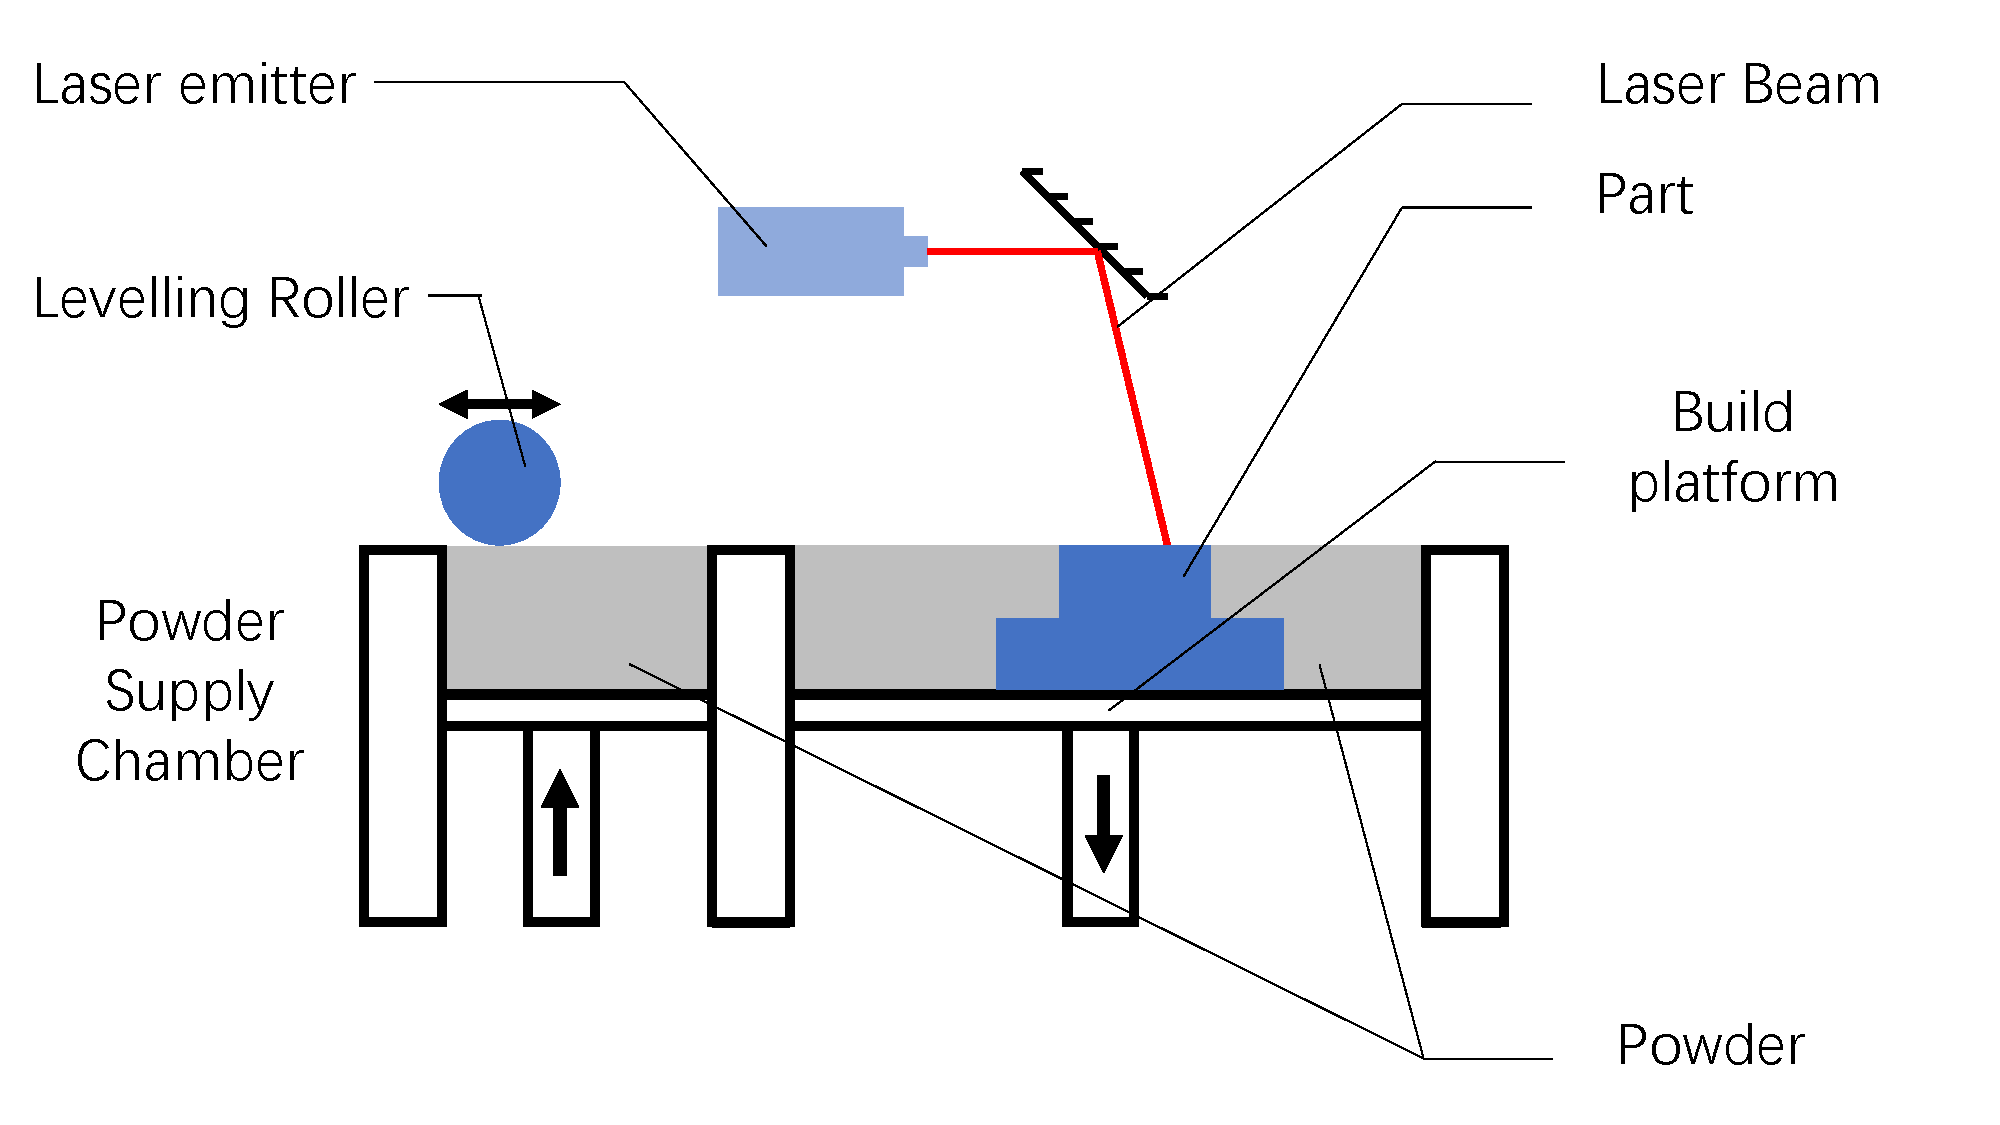
\includegraphics[width=0.9\textwidth]{figures/pbflbm.pdf}
    \caption{Laser-based Powder Bed Fusion of Metals}
    \label{fig: pbflbm}
\end{figure}


Oliverira et al. \cite{Oliveira.2020} have highlighted that two key operational parameters 
exist within the context of \gls{pbflbm}: the source power and the 
scanning velocity. These two parameters exert an influence on the energy 
density imparted to the metal powder, consequently affecting the resulting 
porosity of the fabricated product. Meanwhile, porosity stands as a 
critical parameter impacting the performance of the final product. 
The researchers \cite{Oliveira.2020} have categorized the porosity of the 
finished product into four distinct classes:

\begin{itemize}
    \item Keyhole Porosity: Excessive energy density inhibits the conduction 
    of the melt pool on the powder bed, leading the melt pool to transition 
    into a keyhole mode.
    \item Lack-of-Fusion Porosity: Insufficient energy density results in 
    incomplete fusion of the metal powder, leading to the formation of 
    porosity.
    \item "Balling" (Plateau-Rayleigh instability): Simultaneously employing 
    high source power and excessively elevated scanning velocity induces 
    instability during the processing operation.
    \item Fully-dense porosity: The ideal energy density enables the 
    component to attain a fully dense part.
\end{itemize}


Matthews et al. \cite{Matthews.2017} pointed out that in order to determine 
the evolution of the material's microstructure, information such as 
cooling rate, thermal histories, and material properties are imperative. 
This underscores the necessity of monitoring the \gls{pbflbm} process.

\section{Process monitoring}%
Li et al. \cite{Li.2019} emphasized that in-situ temperature measurement is 
of significant importance for characterizing the mechanical properties of 
materials. In-situ temperature measurement can be categorized into 
in-contact technique and non-contact technique. Given that the temperature 
of the material is high (exceeding 1000$^\circ$C), the region being heated by laser 
is small, and the cooling rate as well as the heating rate is high, 
contact-based measurements would encounter substantial interference, 
thereby rendering the obtained temperature information unreliable. 
Consequently, it becomes essential to employ non-contact-based 
temperature measurement methods.


In the realm of non-contact temperature measurement, 
various measurement systems encompassing ultrasonic, acoustic, and optical 
techniques are present. Within the context of \gls{pbflbm}, 
optical sensors are extensively utilized\cite{Krauss.2012}.


Mani et al. \cite{Mani.2017} pointed out that thermographic imaging in the 
context of Additive Manufacturing (\gls{am}) can be classified into two 
categories based on the optical pathway of the imaging system. 
One category involves aligning the field of view of the sensor with 
the laser beam\cite{Craeghs.2010b,Craeghs.2012,Chivel.2010,Bammer.2010,Berumen.2010,Lott.2011,Yadroitsev.2014}. 
This alignment enables the field of view to track the laser beam, 
allowing for the observation of the melt pool and its scan trajectory.
In addition, an alternative approach involves placing the sensor 
independently of the laser beam. This configuration enables the 
field of view relative static to the material\cite{Craeghs.2012,Dinwiddie.2014,Price.2012,Price.2013,Rodriguez.2012,Wegner.2011}.


Ueda et al. designed the first infrared pyrometer (single-wavelength temperature 
measurement) to measure the temperature. This approach relies on the principles outlined in 
Planck's law, which delineates the interplay between temperature, 
wavelength, and radiative intensity, enabling the measurement of the 
temperature of the object\cite{Ueda.1986}. Subsequently, Dinwiddie et al. 
applied this method for temperature measurement in electron beam melting\cite{Dinwiddie.2014}. 
Meanwhile, Krauss et al. employed this technique to identify defects 
and discontinuous failure spots arising during the \gls{am} process\cite{Krauss.2012}.


However, due to the intricate nature of temperature in real cases, the 
single-wavelength temperature measurement approach may lead to 
misrepresentations of temperature measurement. The models employed in 
single-wavelength temperature measurement methods lack appropriate 
parameters, rendering them susceptible to interference and unable to 
accurately depict the phenomenon of changing emissivity with 
increasing wavelength\cite{Raplee.2017}.





%
%
\section{Multispectral imaging}%

%
%
\section{Emissivity model}%

%
%
\section{Temperature estimation algorithm}


\section{Motivation of this thesis}%
% !TeX spellcheck = en_US
\chapter{Theory and methodology}%
As mentioned in previous sections, forming a virtual experiment platform 
is necessary for investigating the temperature estimation algorithm. So, a virtual 
experiment platform is developed based on Planks'law, then, a virtual multi-spectral 
pyrometer is applied to obtain the digital value (also called image). 


\section{Physical value of radiation}%
Radiation is emitted from any object with a temperature above $0 \, \text{K}$. In equation \ref{eq: radiation_pv}
can be found, that the radiation depends on the black body radiation $B(\lambda, T)$ 
and emissivity $\varepsilon(\lambda, T)$. Both value are temperature $T$ and wavelength $\lambda$ 
dependent.

\begin{equation}
    \label{eq: radiation_pv}
    L(\lambda, T) = B(\lambda, T) \cdot \varepsilon (\lambda, T)
\end{equation}


By Plank's Law, black body radiation can be described in equation \ref{eq: planks_law}, 
with absolute temperature $T$, wavelength $\lambda$, speed of light $c$, Plank 
constant $h$ and Boltzmann constant $k_B$. Black body radiation is irrelevant 
to the material itself, all materials at the same temperature have the same spectral 
black body radiation.

\begin{equation}
    \label{eq: planks_law}
    B(\lambda, T) = \frac{{2hc^2}}{{\lambda^5}} \cdot {\left[{\exp\left(\frac{{hc}}{{\lambda k_B T}}\right) - 1}\right]}^{-1}
\end{equation}


On the contrary, emissivity varies from material to material. It is the 
ratio of the actual spectral intensity emitted by the object to the spectral 
intensity of the black body radiation. In the study of radiation, two idealized 
material models are generally used to describe the idealized 
properties of radiation, namely black body and grey body. 


Black-body material emits electromagnetic black body radiation, which is irrelevant to 
the wavelength of the radiation and the shape of the material\cite{Kuhn.1987}. Which 
also means the emissivity of a black body is constantly 1. It could be used to validate
the temperature estimation algorithm in following sections.


Unlike black-body materials, grey-body materials have an emissivity between 0 and 1.
Not all of the thermal radiation could be emitted to the outside of the material. 
Different from normal materials, the emissivity of a grey-body material is irrelevant
to the wavelength of radiation.

\begin{figure}[htbp]
    \centering
    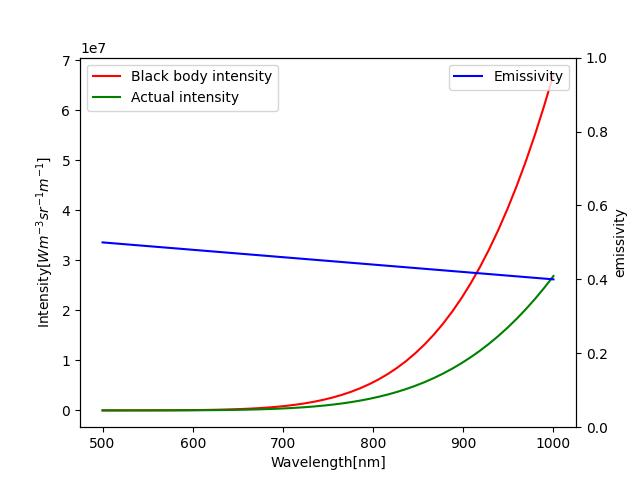
\includegraphics[width = 0.8\textwidth]{figures/real_radiation.jpg}
    \caption{Black body radiation, emissivity and real radiation of an example normal
    material at $1000K$}
    \label{fig: black_body_radiation}
\end{figure}


In Fig.\ref{fig: black_body_radiation} can be found, that the real spectral 
intensity of a normal material is lower than the black body spectral intensity.
And the emissivity of the material varies with the increase of the radiation 
wavelength.


It can be seen that the construction of a reliable emissivity model is crucial to 
the accuracy of the virtual experimental platform. It is the key component used to 
generate the experimental data.




\section{Virtual experiment platform}%
After obtaining the physical spectral intensity of the material, a virtual experiment platform
is used to transform the physical value into digital value, which simulate the 
behavior of a real spectral pyrometer. As described in Fig.\ref{fig: virtual_platform}, a 
camera with a lens system focused on the surface of the powder bed is resonsible 
for obtaining spectral radiation of the heated metal powder. It can be seen from 
Fig.\ref{fig: sensor_pixel}, each pixel of the sensor 
contains 8 filters and thus be able to obtain 8 intensity digital values in different 
channels. Thus, a virtual experiment platform with the same structure as the real 
experiment platform is built.

\begin{figure}[htbp]
    \centering
    \begin{subfigure}{0.6\textwidth}
        \centering
        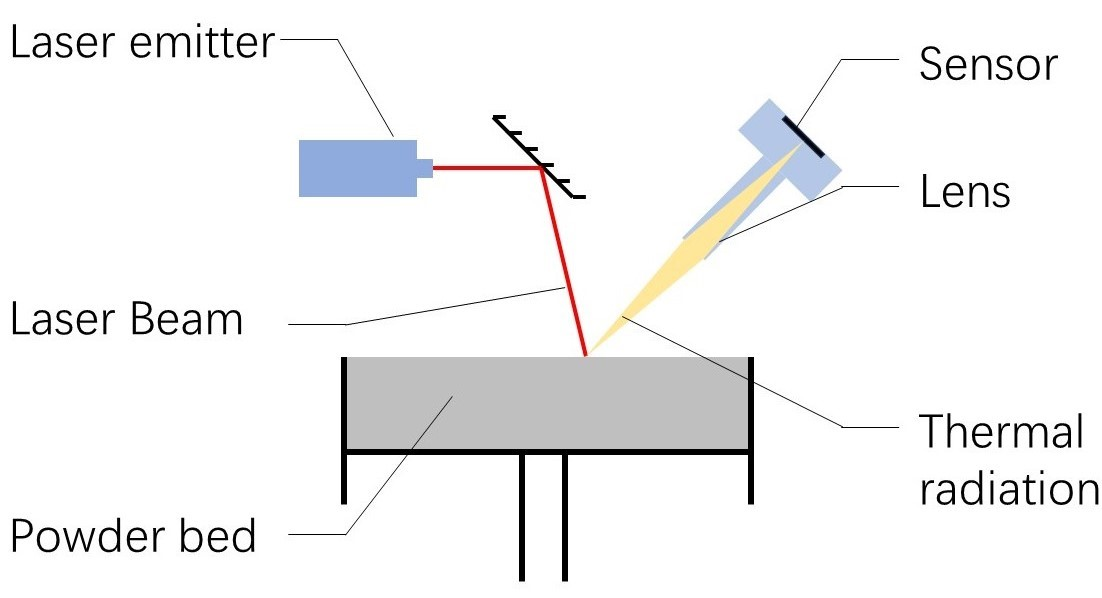
\includegraphics[height=4.8cm]{figures/virtual_platform.jpg}
        \caption{Virtual experiment platform}
        \label{fig: virtual_platform}
    \end{subfigure}
    \hfill
    \begin{subfigure}{0.37\textwidth}
        \centering
        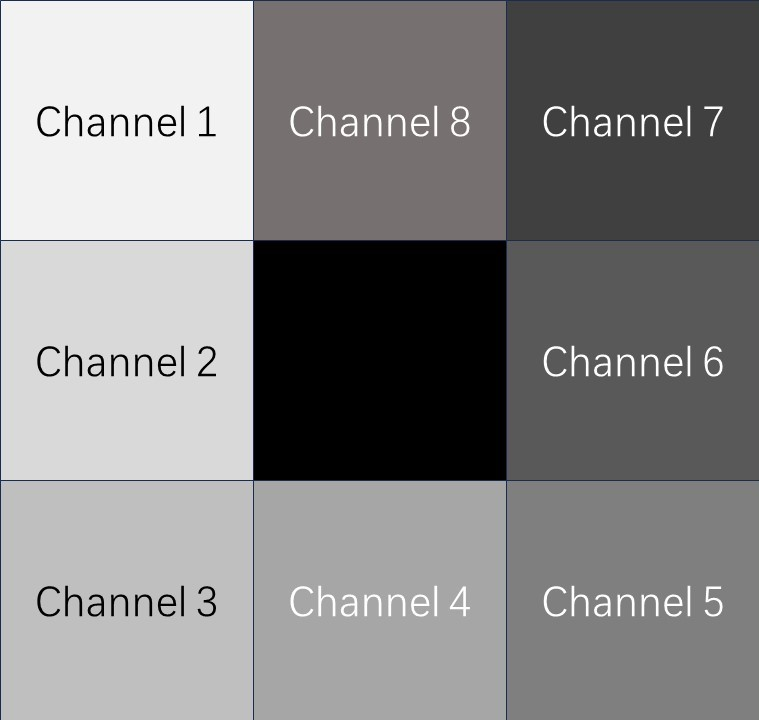
\includegraphics[height=5cm]{figures/sensor_pixel.jpg}
        \caption{Layout of a sensor pixel}
        \label{fig: sensor_pixel}
    \end{subfigure}
    \caption{Structure of the virtual experiment platform and Layout of a sensor pixel}
    \label{fig: virtual_pixel}
\end{figure}


\section{Camera model}
It can be found in Fig.\ref{fig: virtual_pixel}, The thermal radiation is emitted from the surface of powder bed, and passes through 
the lens system of the camera, finally, it reaches the sensor and be converted into 
digital values. The simplified process can be seen in Fig.\ref{fig: view_factor}. $dA_m$ is the 
area of the focused surface and $dA_{pixel}$ the area of the pixel in camera system, $n_m$ is the 
normal vector of the surface.

\begin{figure}[htbp]
    \centering
    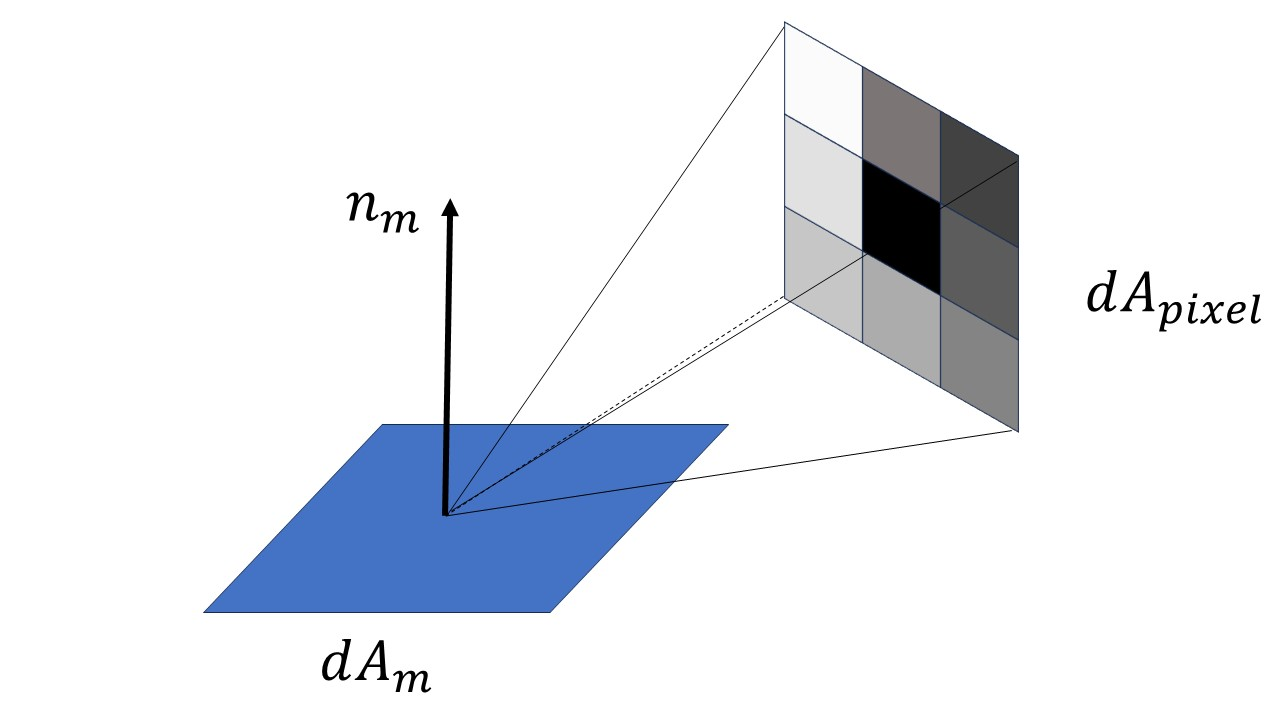
\includegraphics[width=0.6\textwidth]{figures/view_factor.jpg}
    \caption{Radiative exchange between camera system and powder bed}
    \label{fig: view_factor}
\end{figure}


\begin{comment}
Thus, the radiation intensity received by the camera system can be expressed in Eq.\ref{eq: physical_value_received}.
Where $dL_{sensor}$ means the spectral intensity reached on each channel, $dL_{material}$
is the spectral intensity emitted from the surface area, $\phi_{dA_m - dA_{pixel}}$ is the 
view factor between the focused surface area and camera system.

\begin{equation}
    \label{eq: physical_value_received}
    dL_{sensor} =  dL_{material} \cdot \phi_{dA_m - dA_{pixel}}
\end{equation}


The view factor describes the ratio between the emitted intensity of the surface area 
and the received intenisty by the pixel in camera. It only relates to the shape of 
the two surfaces and the geometric position between them\cite{Rohsenow.1998}. Since 
in real experiments, the sensor is fixed in a certain position on the machine while the 
surface of the powder bed does not move relatively to the machine, it can be concluded
that the geometry of the camera system and the focused area does not change. This means that 
the view factor does not change as the process proceeds.


So, in order to simplify the physical model of the virtual experiment platform and 
thus avoid unnecessary complexity, one assumption was made that the view factor between 
surface area of the powder bed and the camera system is constantly set to 1.
\end{comment}


\subsection{Frequency response}
After obtaining the virtual experiment platform and knowing the external setup of the 
sensor, the internal effects of the camera system should also be taken into account 
in the complete virtual experiment platform.


In order to simulate real camera system, the frequency response of sensor and lens 
should be considered. In real camera systems, all spectral radiation will 
pass through the lens system of camera. Since the lens system is not an 
idealized system, the effect of the lens system is not negligible. 

\begin{figure}[htbp]
    \centering
    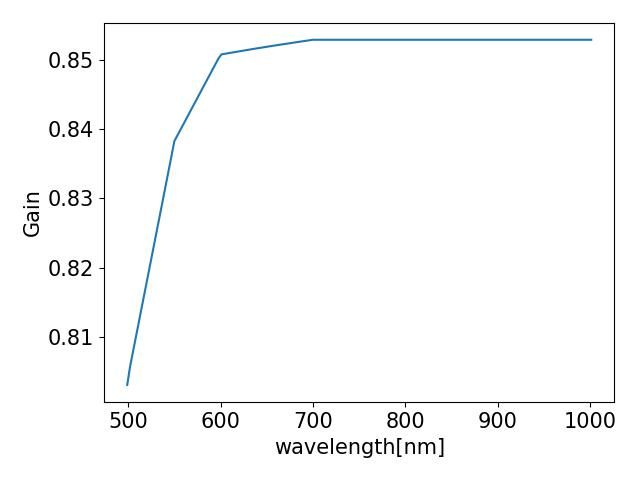
\includegraphics[width=0.6\textwidth]{figures/tr_frequency_response.jpg}
    \caption{Frequency response of the lens system}
    \label{fig: frequency_response_lens}
\end{figure}


It can be found in Fig.\ref{fig: frequency_response_lens} that system gain 
of lens system is not constant. In the wavelength range of 500 to 700 nanometers, 
the lens is more sensitive to the radiation with long wavelength. With the 
increasing wavelength, the system gain of the lens system keep constant at 0.853.


In addition to the fact that the lens system respond differently to radiation
with different wavelengths, the sensor of the camera also have wavelength-dependent quantum 
efficiency. As mentioned in previous section, the acquisition of the spectral 
intensity by the sensor for different channels is based on the filter 
before the pixels. 


Fig.\ref{fig: quantum_efficiency} shows the quantum efficiency 
of the camera sensor in different channels. Unlike an ideal sensor that 
receives only single wavelength radiation, the intensity information received 
by a real sensor is a combination of a spectral radiation and 8 filters with 
different frequency responses. Thus, the camera system is able to obtain the 
spectral radiation intensity in 8 channels simutaneously. 


\begin{figure}[htbp]
    \centering
    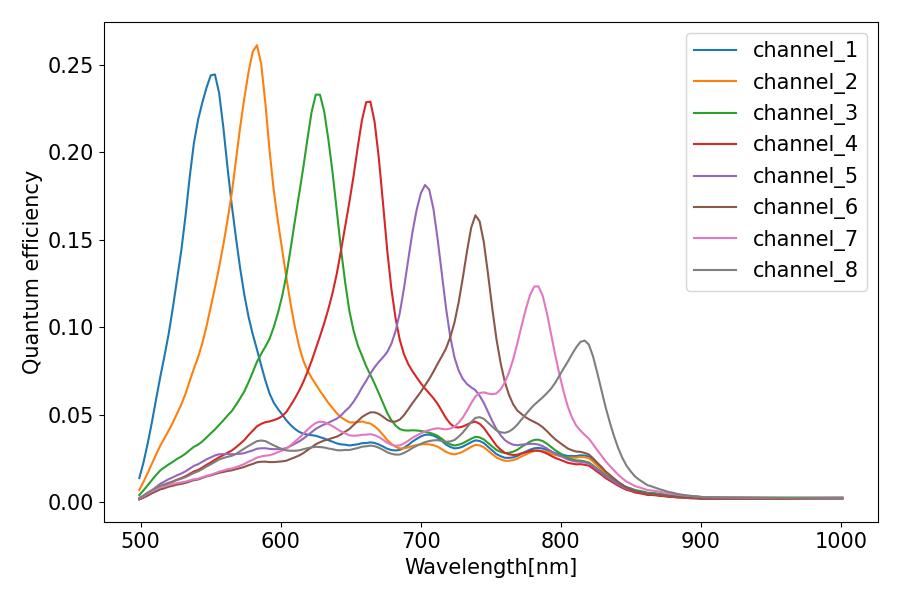
\includegraphics[width = 0.8\textwidth]{figures/quantum_efficiency.jpg}
    \caption{Quantum efficiency of camera system in each channel}
    \label{fig: quantum_efficiency}
\end{figure}


To make the virtual experiment platform more comparable to real experiments, 
it can be concluded that it is necessary to build a camera model that 
incorporates the effects of sensor quantum efficiency and lens transparency.
Then, the physical value of the spectral radiation intensity could be 
calculated accurately by the digital value of spectral radiation intensity obtained from the virtual experiment 
platform.


\subsection{Integration method}
As a result, the process of converting the physical values of radiation intensity 
into digital values needs to be accurately reproduced. Since the total efficiency 
of the camera (${\eta}_{camera}$) was delivered by quantum efficiency (${\eta}_{quantum}$)
of the sensor and transparency of the lens system{$\tau_{lens}$}, the mathematical
relationship could be described in Eq.\ref{eq: cam_efficiency}.


\begin{equation}
    \label{eq: cam_efficiency}
    {\eta}_{camera} = {\eta}_{quantum} \cdot \tau_{lens}
\end{equation}


Fig.\ref{fig: received} shows the relationship between the incoming spectral 
radiation intensity and actual captured spectral radiation intensity 
by the camera system. It can be found that the wavelength of the spectral 
radiation intensity actually received by the sensor deviates from the wavelength of the 
spectral radiation intensity it supposed to receive.


\begin{figure}[htbp]
    \centering
    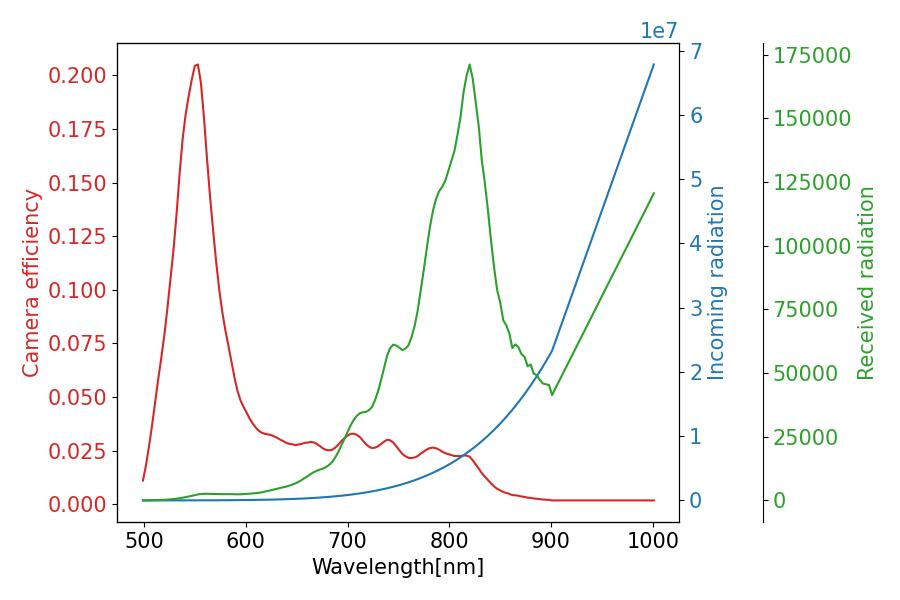
\includegraphics[width = 0.8\textwidth]{figures/received_radiation.jpg}
    \caption{Actual received spectral radiation intensity by channel 1 at 1000K}
    \label{fig: received}
\end{figure}


Obtaining the physical value of spectral radiation intensity, the sensor is responsible 
for transforming the physical value into digital value for upcoming proceedings.
The camera system used in real experiment platform uses \gls{ccd} or \gls{cmos}
as their sensors. Both sensors transform the photon flux $\phi (\lambda)$ 
incident on the semiconfuctor into photocurrent $I_{ph}$\cite{Fossum.2014}. 

\begin{equation}
    \label{eq: principle_cmos}
    I_{ph} = q \int_{\lambda}^{} \phi(\lambda) \cdot \eta_{camera}(\lambda) d\lambda
\end{equation}

With a certain temperature $T$: 

\begin{equation}
    \label{eq: quantum_flux_intensity}
    \phi(\lambda) = L(\lambda, T)
\end{equation}

Eq.\ref{eq: principle_cmos} is the mathetical description of the 
transformation. Where $\phi(\lambda)$ denotes photon flux on the sensor, 
which is equal to the spectral radiation intensity on the sensor $L(\lambda, T)$ as 
described in Eq.\ref{eq: quantum_flux_intensity}, and $\eta_{camera}(\lambda)$
denotes the total efficiency of the camera in Eq.\ref{eq: cam_efficiency}. $q$ is the sensitivity parameter 
of the sensor.


\subsection{Implementation}
Similar to the method used to obtain the digital value of spectral radiation intensity 
in the real experiment, the virtual experiment platform calculates the 
intensity digital value in 8 channels using the virtual camera by entering 
the material properties of the point being measured.


\begin{figure}[htbp]
    \centering
    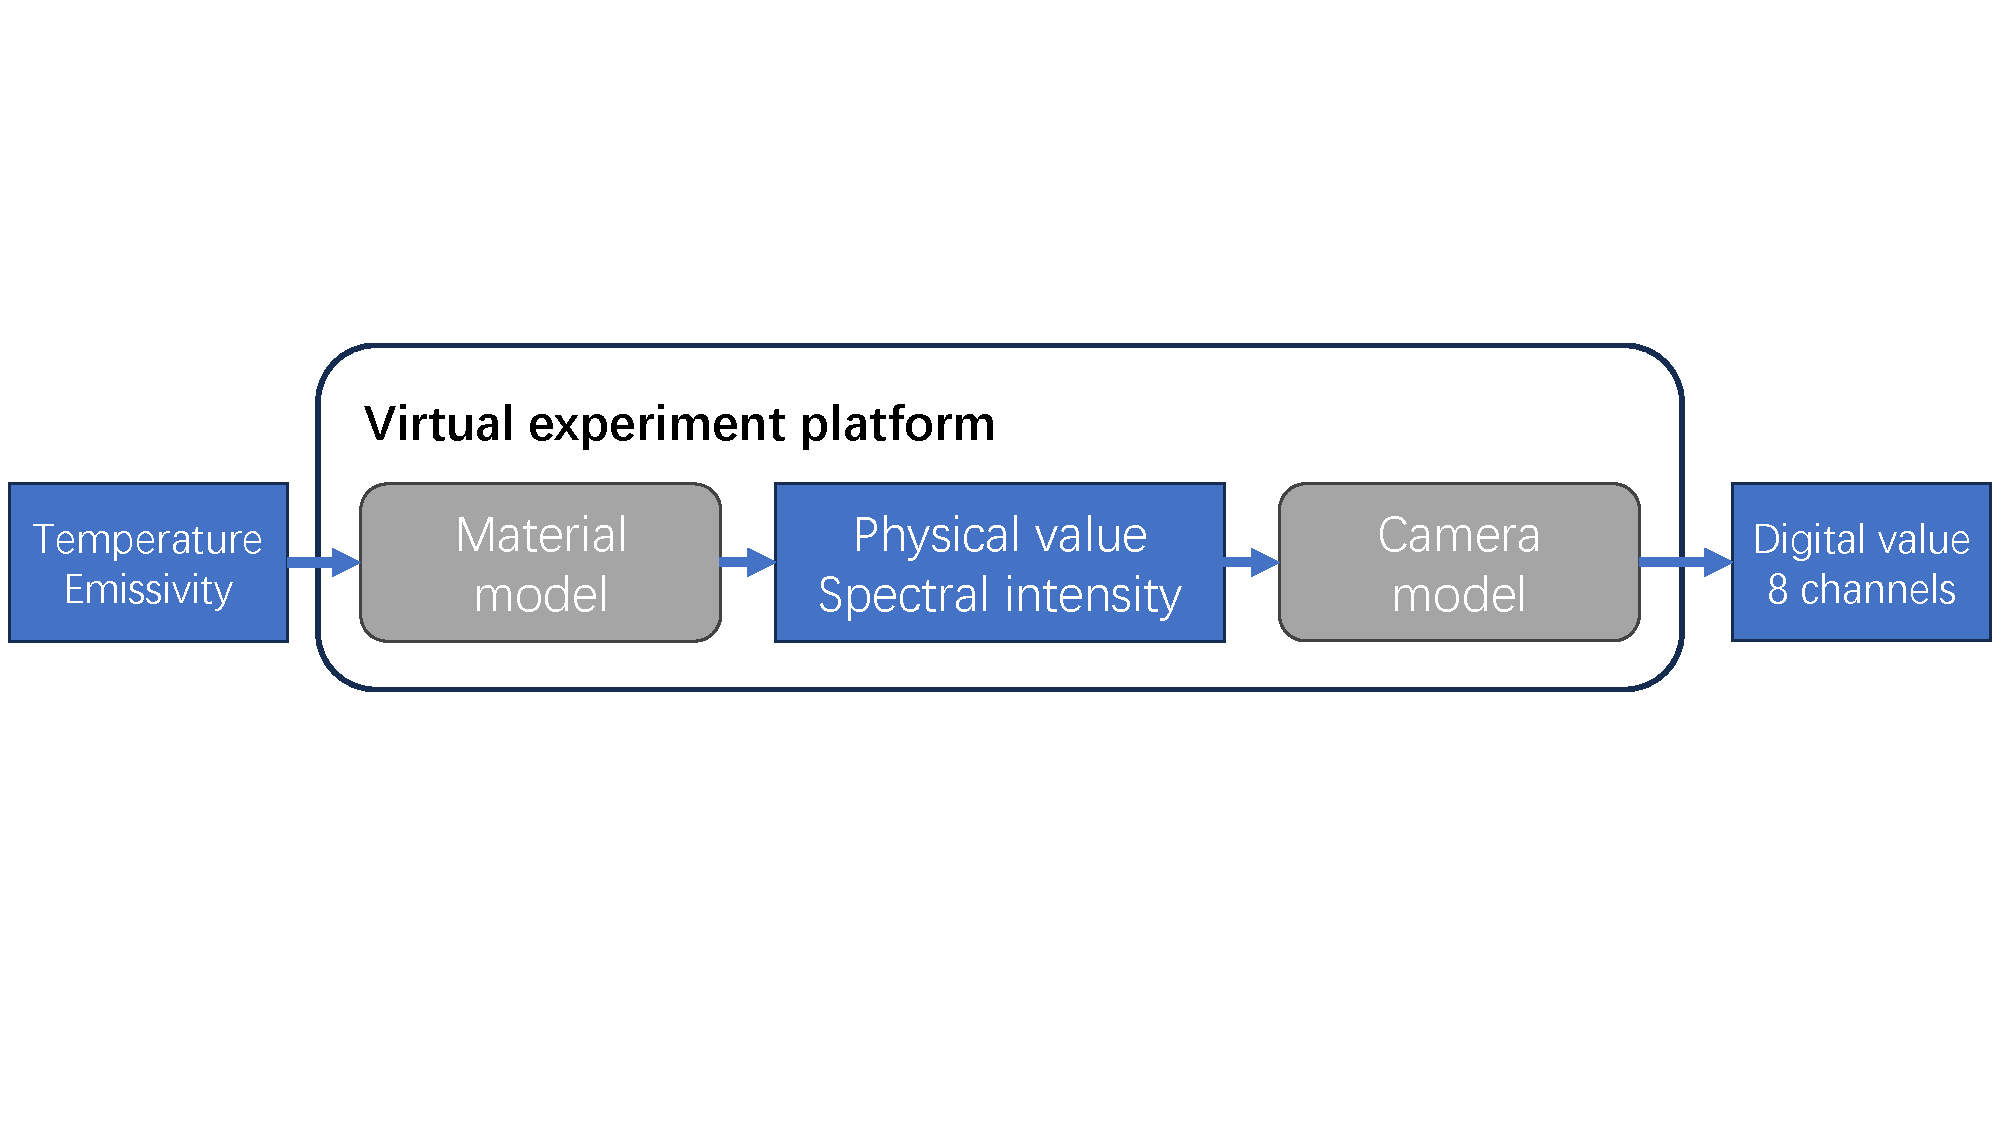
\includegraphics[width=0.95\textwidth]{figures/camera_model.pdf}
    \caption{Procedure of using virtual experiment platform to generate digital values}
    \label{fig: process_virtual_platform}
\end{figure}

Fig.\ref{fig: process_virtual_platform} shows the working procedure of the 
virtual experiment platform. 
To enable the virtual experimental platform to run on various devices, 
the entire platform has been implemented using Python as the 
programming language and packaged into a .py file. Furthermore, all 
functions have been vectorized to facilitate the generation of image 
outputs resembling those captured by a physical camera. Additionally, 
the parallel computing package in Python has been utilized to minimize 
computation time.


\section{Temperature estimation algorithm}
After obtaining the experimental data calculated by the virtual experiment platform, 
a temperature estimation algorithm should be developed to calculate the temperature 
of the measured point based on the experimental data.


Similar to the set up in real experiments, the parameters of the camera model can be 
considered as known in the virtual experimental platform mentioned in this article. 
This will on the one hand improve the accuracy of the temperature estimation algorithm
and on the other hand avoid some unnecessary complexity.


Thus, in this temperature estimation algorithm, the known variable is the digital value of 
spectral intensity captured by camera model in virtual experiment platform, the characteristic 
of the camera system. The variables to be estimated are the temperature of the measured point and 
its emissivity.


\begin{figure}[htbp]
    \centering
    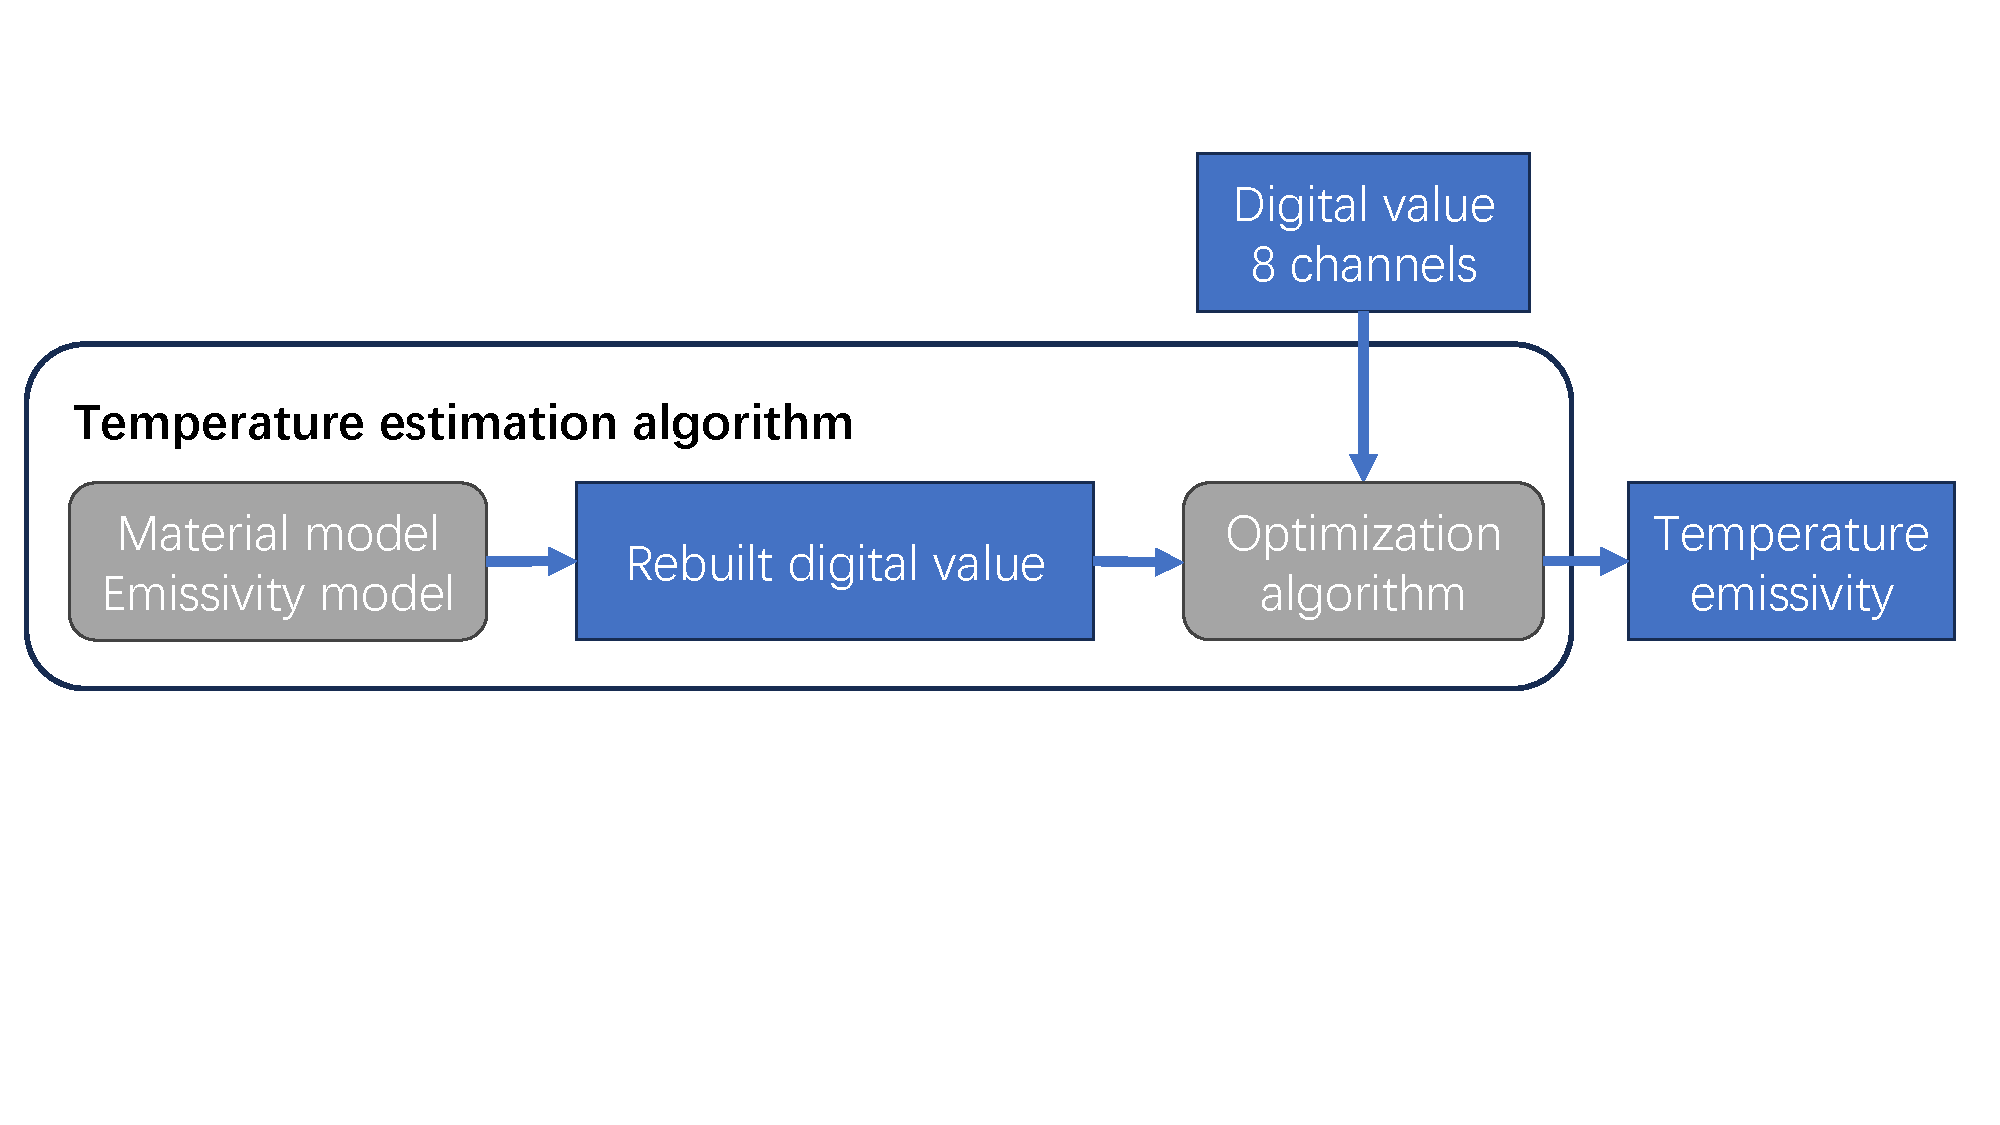
\includegraphics[width=0.95\textwidth]{figures/temperature_esti_algorithm.pdf}
    \caption{Procedure of temperature estimation algorithm}
    \label{fig: temperature_estimation_algorithm}
\end{figure}


\subsection{Temperature estimation with integration method}
Fig.\ref{fig: temperature_estimation_algorithm} shows the proceeding procedure of the 
temperature estimation algorithm. The digital value of the spectral radiation intensity
$(I_{rec}(i))$ 
in the $i_{th}$ channel should be reconstructed in Eq.\ref{eq: reconstruct_integration}:

\begin{equation}
    \label{eq: reconstruct_integration}
    I_{rec}(i) = q \int B(\lambda, T) \cdot \varepsilon(\lambda, k, T) \cdot \eta_{camera}(i) d\lambda
\end{equation}

With $I_{DV}(i)$ the reconstructed digital value in $i_{th}$ channel, $B(\lambda, T)$ the black body radiation, 
$\varepsilon(\lambda, k, T)$ the emissivity model in temperature estimation algorithm, 
$\eta_{camera}(i)$ the total camera efficiency of $i_{th}$ channel. It can be found that 
the emissivity model have an additional parameter $k$, this parameter is used for fitting 
the emissivity behavior of the measured material. More details can be found in the following 
section.


Given an initial guess of the status parameters, namely 
temperature($T_0$) and parameters in emissivity model($k_0$). Then, an curve fit 
algorithm is applied to minimize the difference between the reconstructed digital value $(I_{rec})$ 
and the actual digital value $(I_{act})$ in Eq.\ref{eq: reconstruct_optimization}.

\begin{equation}
    \label{eq: reconstruct_optimization}
    \min_{k, T}\sum_{i=1}^{8}  F(I_{rec}(i), I_{act}(i))
\end{equation} 

$F(I_{rec}(i), I_{act}(i))$ is the cost function of the curve fit algorithm. In this 
application, Non-linear least squares method is used to obtain the optimum parameters 
as Eq.\ref{eq: least_square}.

\begin{equation}
    \label{eq: least_square}
    F(I_{rec}(i), I_{act}(i)) = (I_{rec}(i) - I_{act}(i))^2
\end{equation}


After obtaining the estimated temperature ($T_{estimate}$) and the parameter ($k$) 
in the emissivity model, the data will be saved in a .xlsx file for 
potential operations.

\subsection{Temperature estimation with linear method}
To be done


\section{Emissivity model in temperature estimation algorithm}%
As an unknown quantity in the temperature estimation algorithm, the nature of emissivity 
as a function of wavelength also introduces an additional degree of freedom 
into the overall calculation process. In order to provide a more general description of 
the trend of emissivity with wavelength, an additional parameter ($k$) in the 
emissivity model used for temperature estimation has been introduced.


Due to the inherent complexity of this trend, it is often impossible to describe 
the emissivity using a single parameter. Therefore, the parameter ($k$) is normally 
represented as a vector composed of multiple variables. This approach allows for both a 
concise mathematical representation and the incorporation of more 
intricate emissivity models into the temperature estimation algorithm.


%
%
%
\chapter{Application}

After the theoretical basis of the virtual experiment platform is known and 
the program of the virtual experiment platform is built, the application should be 
verified with experiment data generated based on the real experiment.


\begin{figure}[htbp]
    \centering
    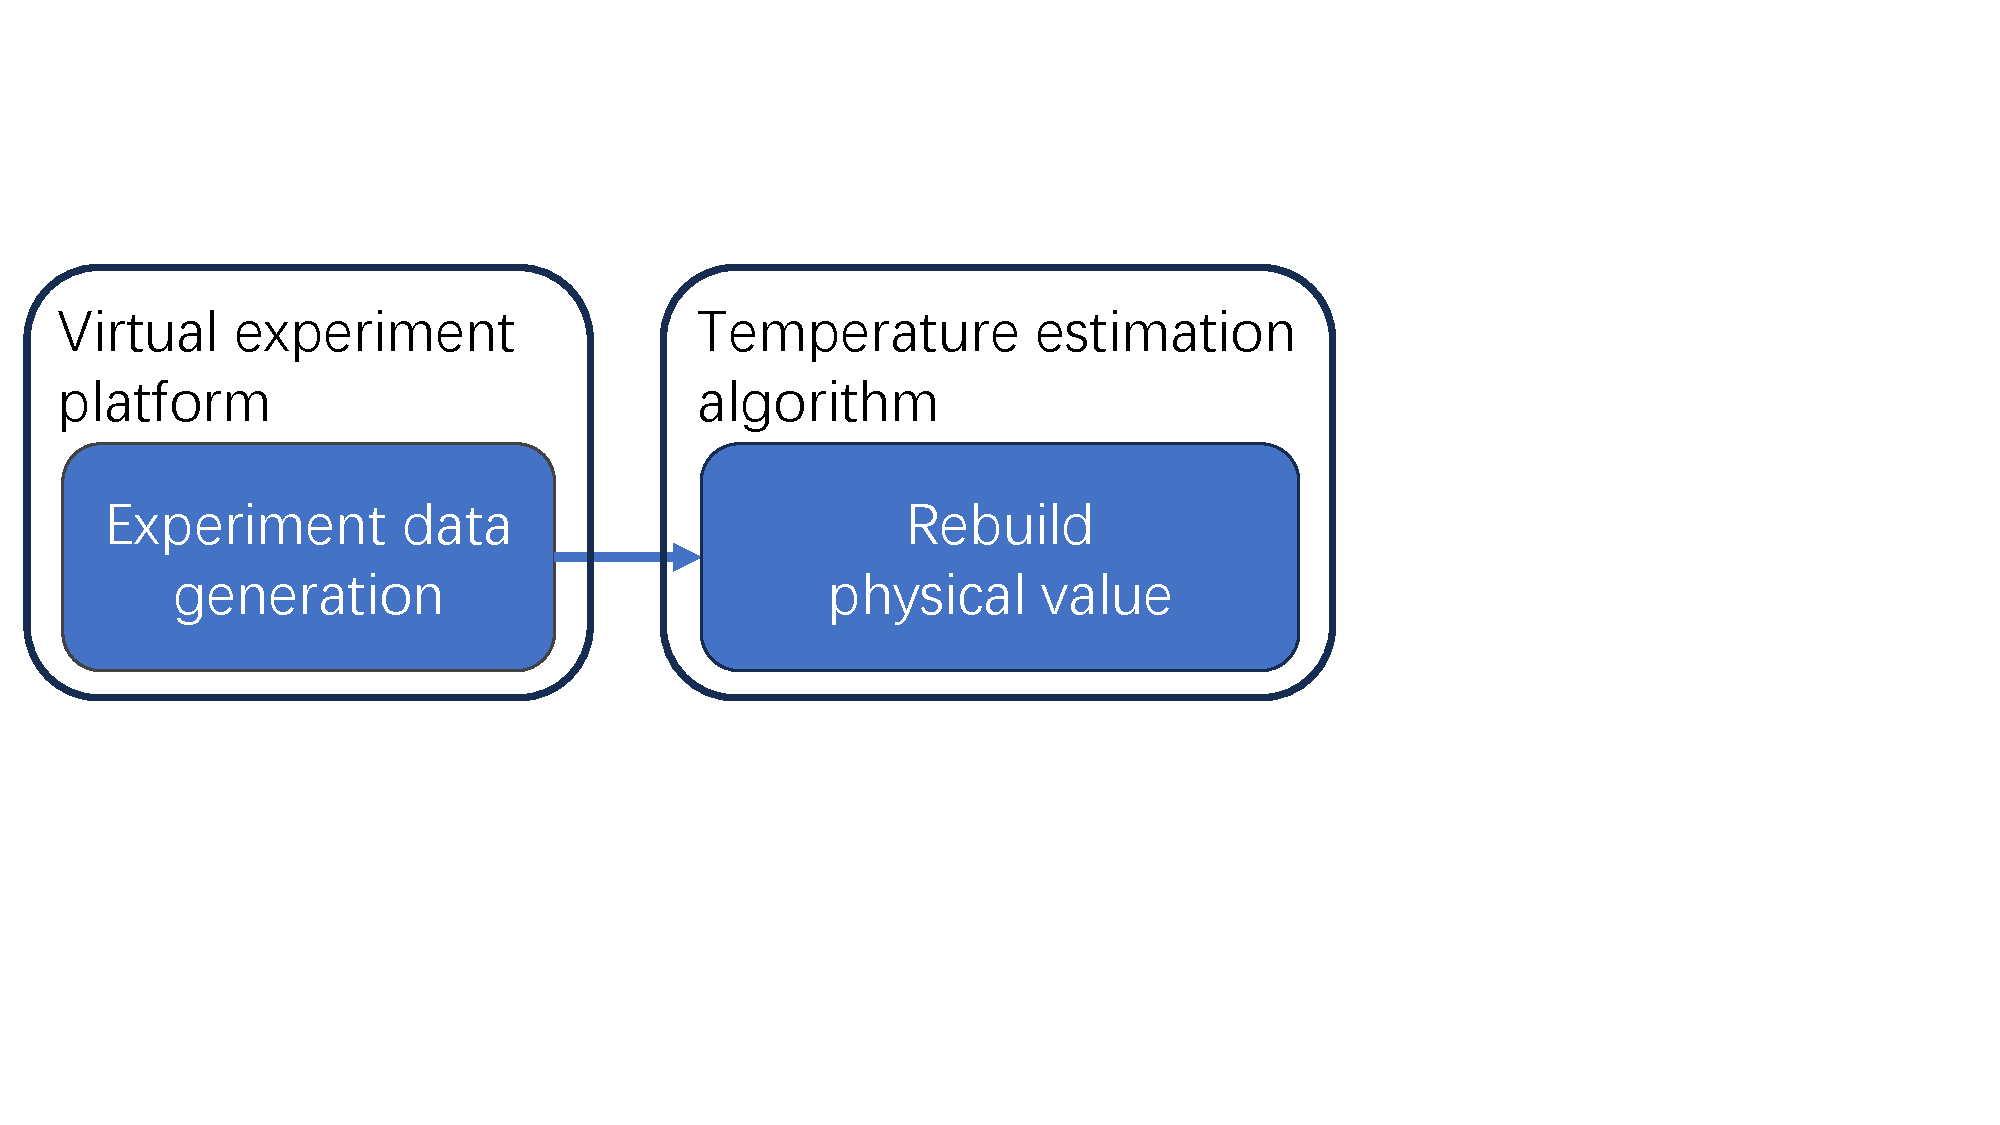
\includegraphics[width=0.6\textwidth]{figures/application_procedure_1.pdf}
    \caption{Complete procedure from data generation to model validation}
    \label{fig: application_procedure}
\end{figure}


Fig.\ref{fig: application_procedure} shows the procedure of the application.
Firstly, an experiment data set should be generated according to the parameters of the 
hypothetical material. Then, a temperature estimation algorithm is applied to 
estimate the temperature of the hypothetical material. Last, a validation procedure 
is used to check the accuracy and stability of the results of 
temperature estimation algorithm.


As mentioned in previous sections, these functions is implemented in three 
programmes. Namely virtual experiment platform, temperature estimation algorithm
and validation procedure. Similar to conventional experiment methods, these
steps are independent procedures, which means they do not interact with 
each other. 


Accordingly, this chapter will be divided into three sections, which describe 
the implementation and the parameter settings of the virtual experiment platform, 
temperature estimation algorithm and validation procedure.


\section{Experiment data generation}
As the first of the three steps mentioned above, it is crucial to generate 
accurate experimental data correctly. It affects the comparability of the 
virtual experimental platform with real experiments on the one hand, and 
the accuracy of the temperature estimation algorithm on the other. As a 
result, the virtual experimental platform should be able to perform 
calculations for as many hypothetical materials with different properties 
as possible.


In order to be able to obtain image similar to image from
real camera, the area that the virtual camera is able to capture is 
set to a 50*50 pixel picture. Fig.\ref{fig: camera} shows the image obtained 
from real experiment and virtual experiment platform. The major difference between 
these two images is the coloring. In real experiment, the raw image was saved 
as a .tiff file, which obtain the spectral intensity received by the specific 
channel. Then, the intensity is expressed as brightness of the pixel in the display of 
the image. This results in the experiment data that is not intuitive and 
requires specialised software to open these data.


As a result, there are a number of optimisations that have been applied 
in this virtual experiment platform. Firstly, the raw digital value 
of the received spectral intensity was saved in an .xlsx file, which 
simplifies the reading of the data as well as the conversion. In 
addition, a .jpg image of each channel similar to the real experiment data is also 
saved. Different from the real experiment data, colours are used here to 
indicate the value of the spectral intensity. This improves the 
readability of the experiment data.


\begin{figure}[htbp]
    \centering
    \begin{subfigure}{0.45\textwidth}
        \centering
        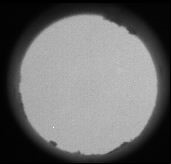
\includegraphics[height=5cm]{figures/real_camera_1075.JPG}
        \caption{Real experiment data  (channel 1)}
        \label{fig: real_camera}
    \end{subfigure}
    % \hfill
    \begin{subfigure}{0.45\textwidth}
        \centering
        
\includegraphics[height=5cm]{figures/virtual_camera_1098.jpg}
        \caption{Virtual experiment data (channel 1)}
        \label{fig: virtual_camera}
    \end{subfigure}
    \caption{Comparison between real experiment data at $1300K$ (a)
    and virtual experiment data at $1098K$ (b)
    }
    \label{fig: camera}
\end{figure}


Thus, the observation area is obtained by initialization of the the virtual 
experiment platform. Temperature field, emissivity model of the hypothetical 
material and the integration method are the parameters to be defined as the next
step.


\subsection{Temperature field}%
As mentioned in previous sections, temperature is one of the most important parameters 
in the virtual experiment platform. In order to obtain results similar to real 
experiments, a temperature field exists in the observation area. For the purpose of 
simplifying the calculation process, this temperature field consists of two main 
regions, a background region at the edge of the observation area, 
where the temperature is uniformly set to 1000K, and an internal high temperature 
region, where the temperature follows a predefined distribution.


\begin{figure}[htbp]
    \centering
    \begin{subfigure}{0.08\textwidth}
        \centering
        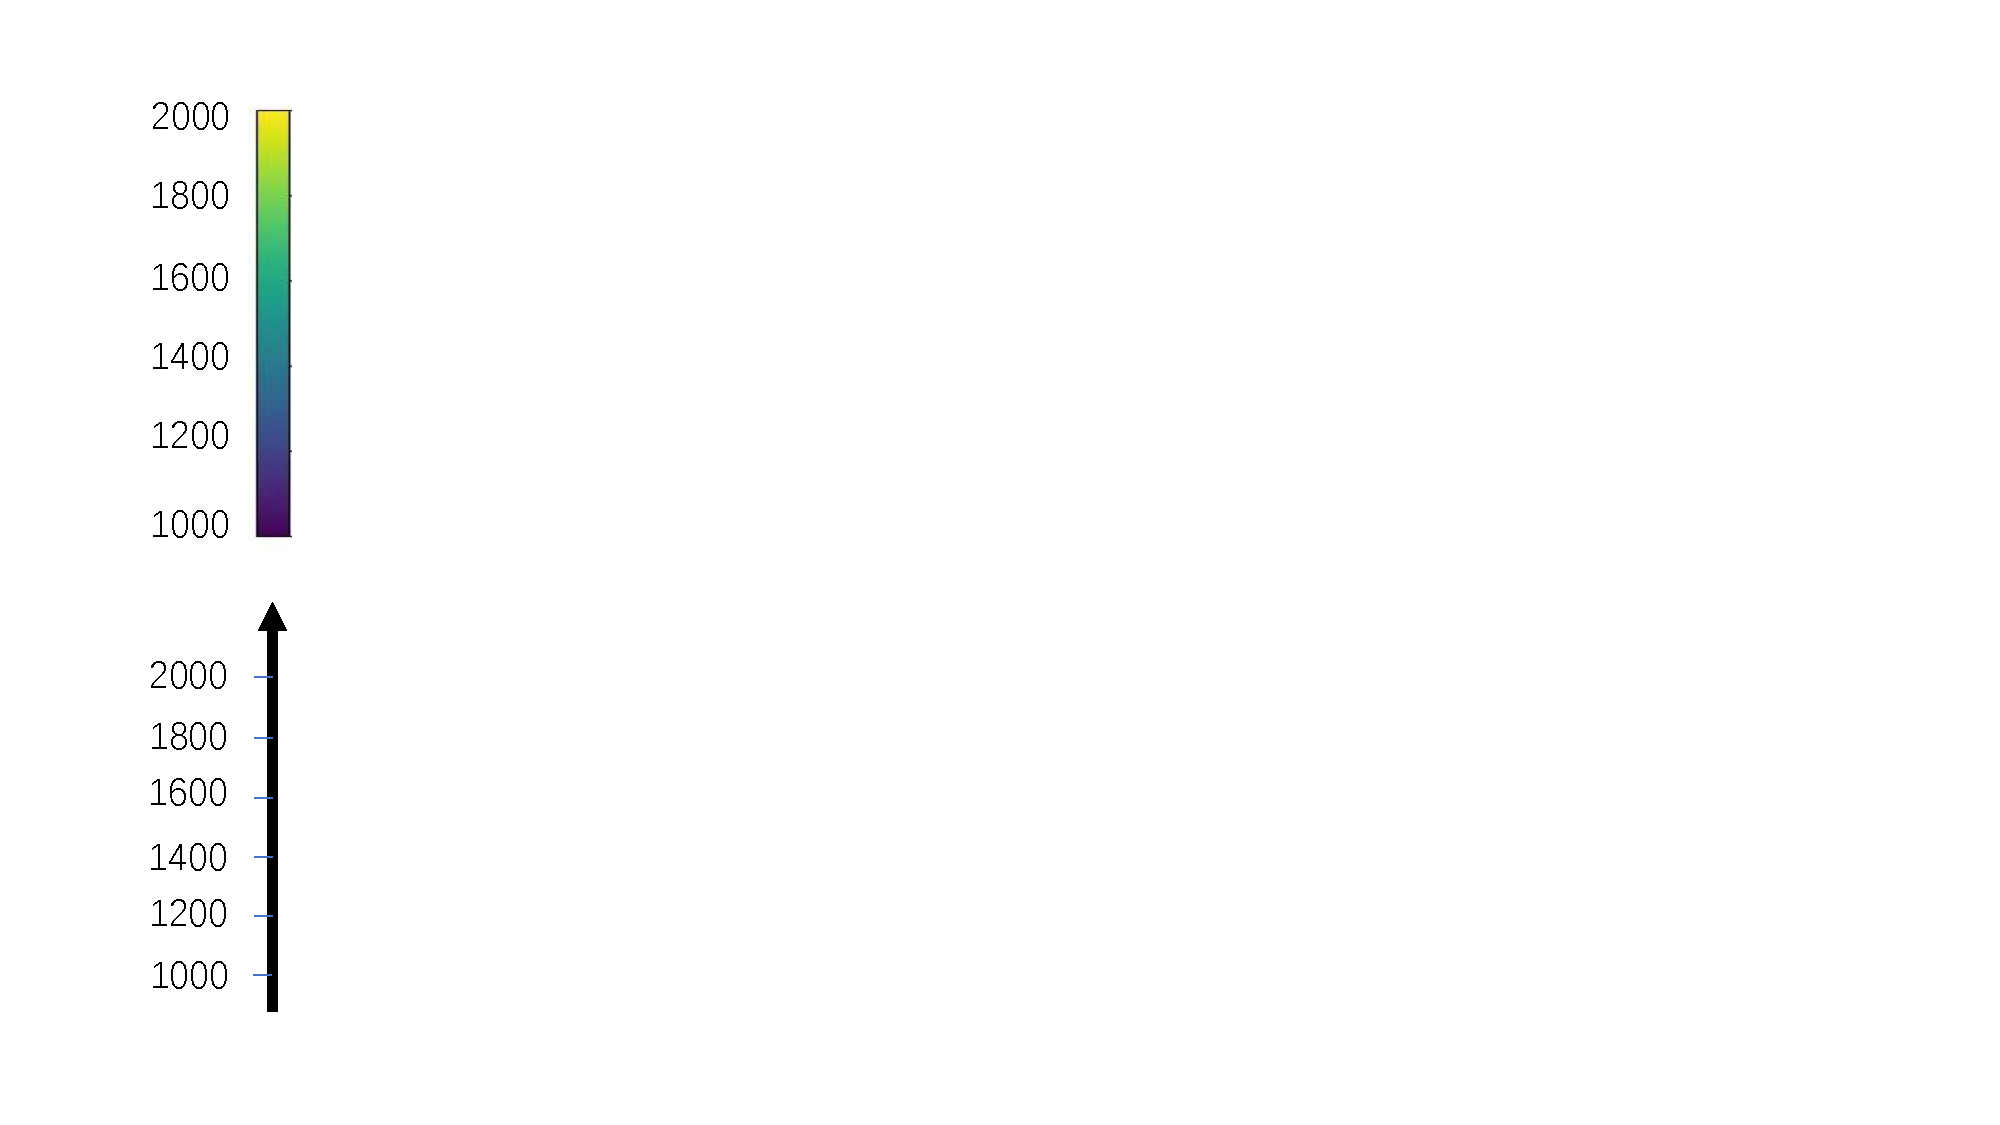
\includegraphics[height=9cm]{figures/temp_distribution_colorbar.pdf}
        \caption*{}        
    \end{subfigure}
    \begin{subfigure}{0.3\textwidth}
        \centering
        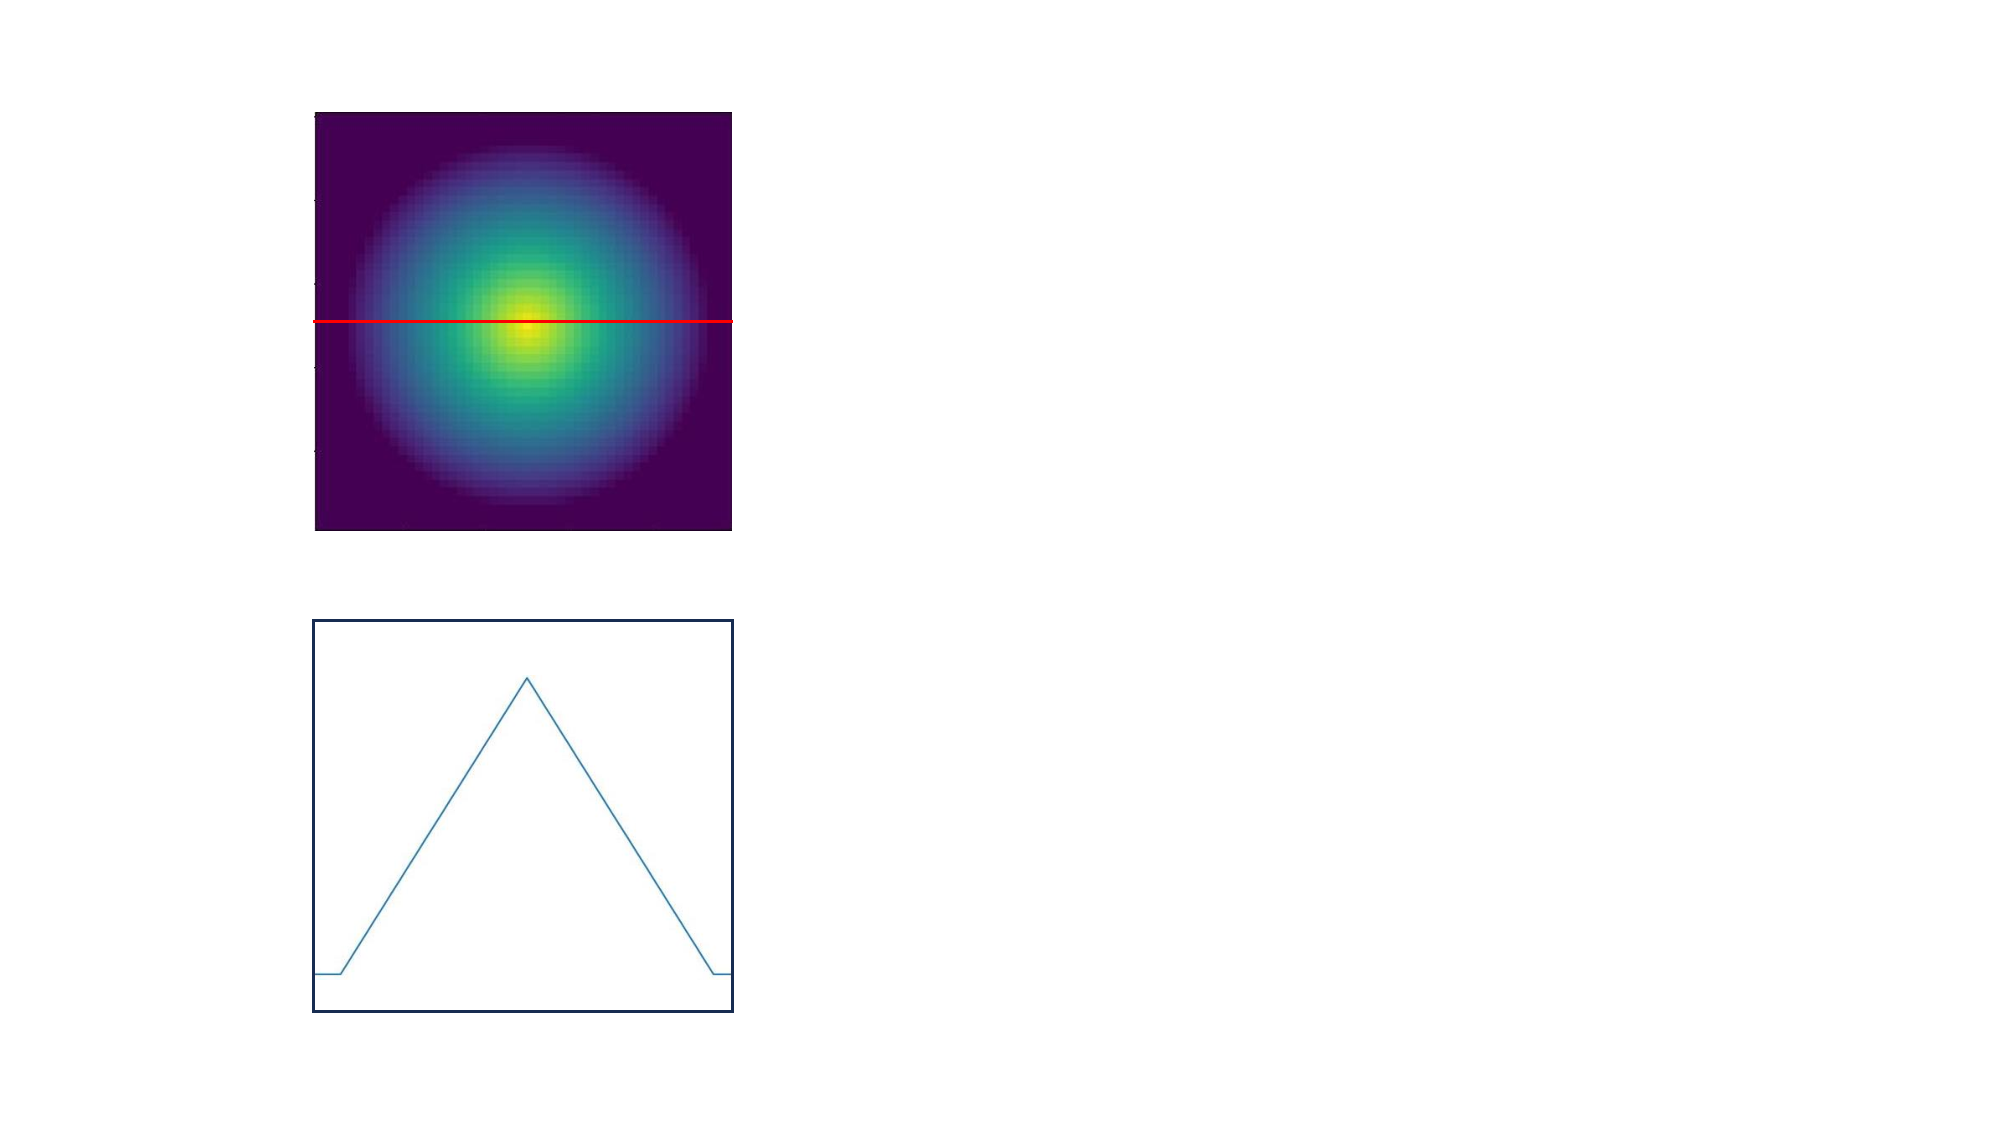
\includegraphics[height=9cm]{figures/temp_distribution_a_1.pdf}
        \caption{Linear}
        \label{fig: linear_distribution}        
    \end{subfigure}
    \begin{subfigure}{0.3\textwidth}
        \centering
        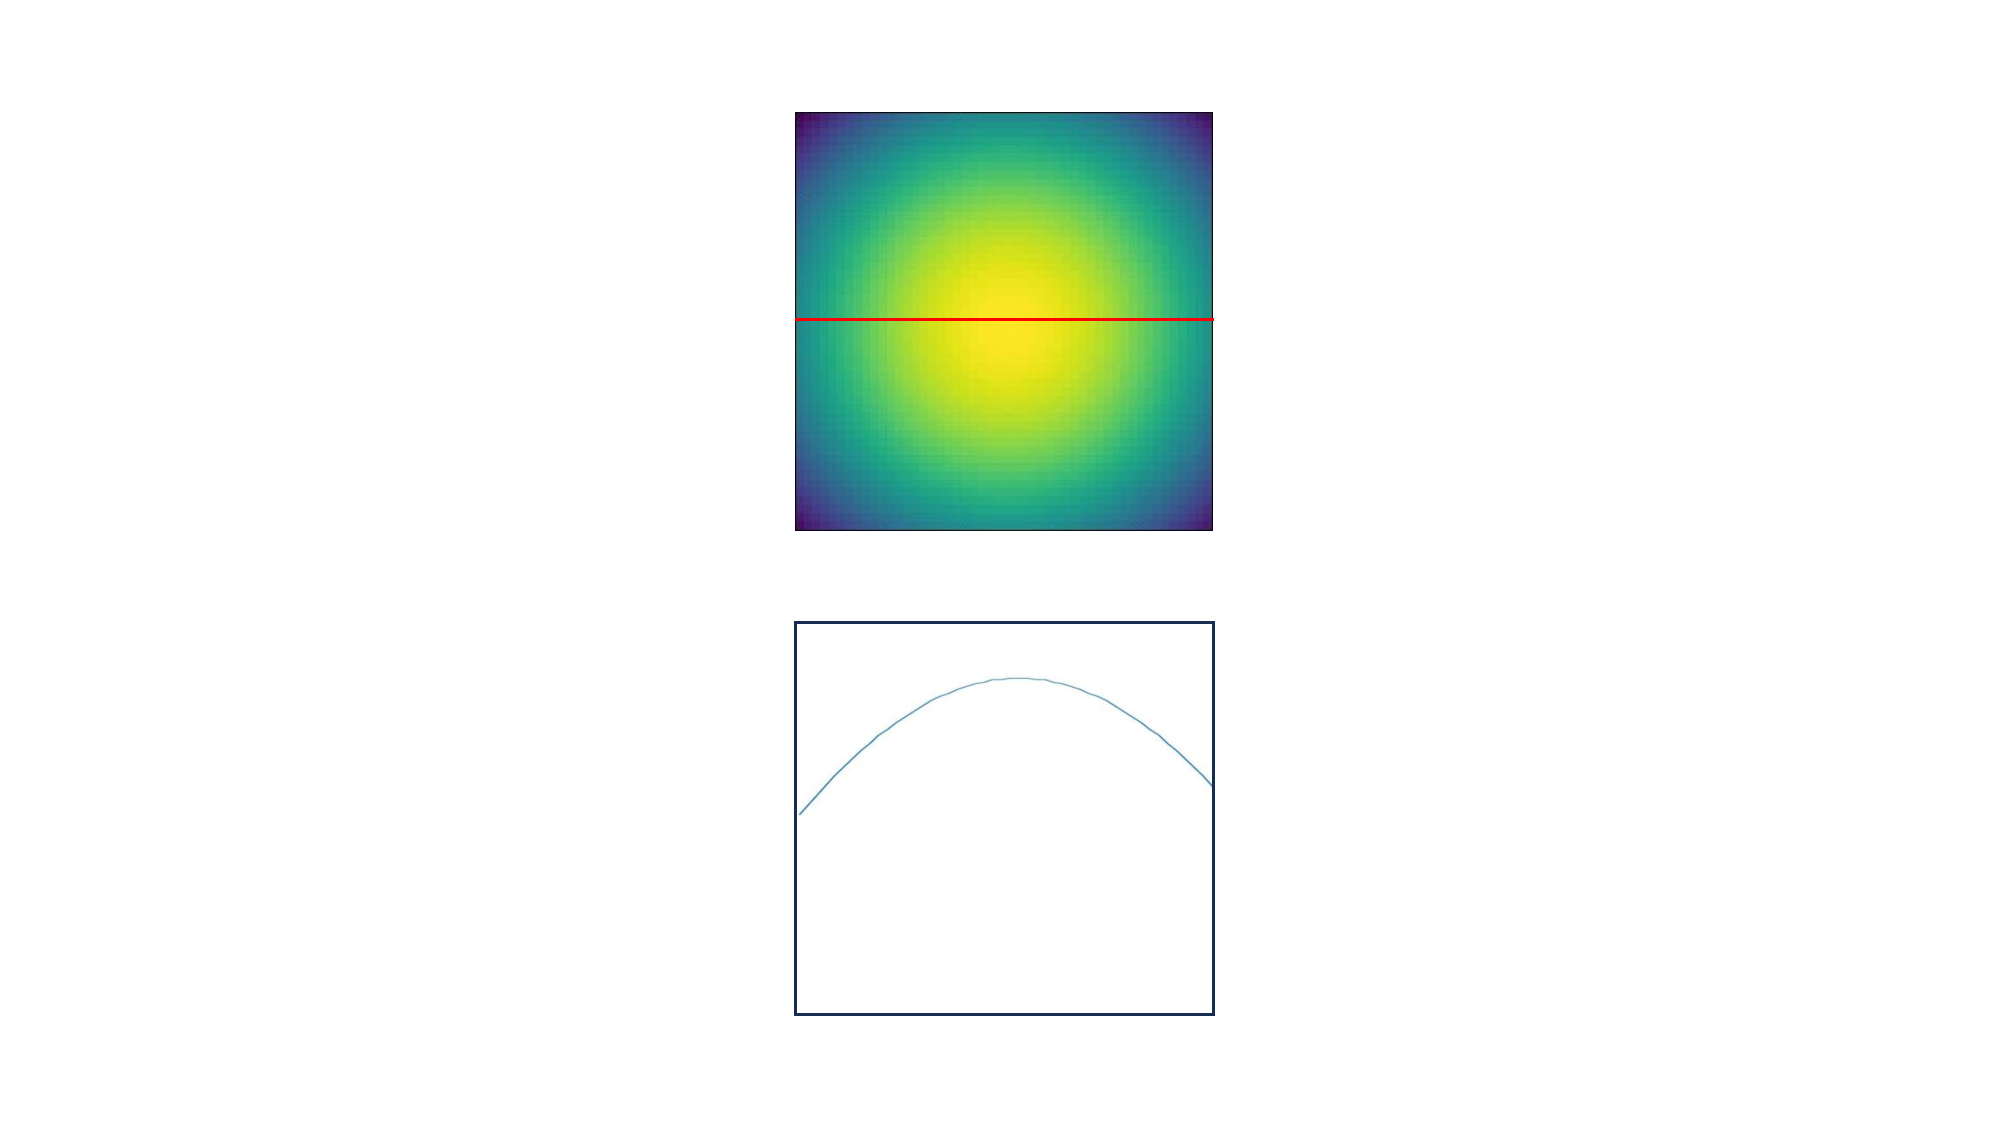
\includegraphics[height=9cm]{figures/temp_distribution_b_1.pdf}
        \caption{Gaussian}
        \label{fig: gaussian_distribution}        
    \end{subfigure}
    \begin{subfigure}{0.3\textwidth}
        \centering
        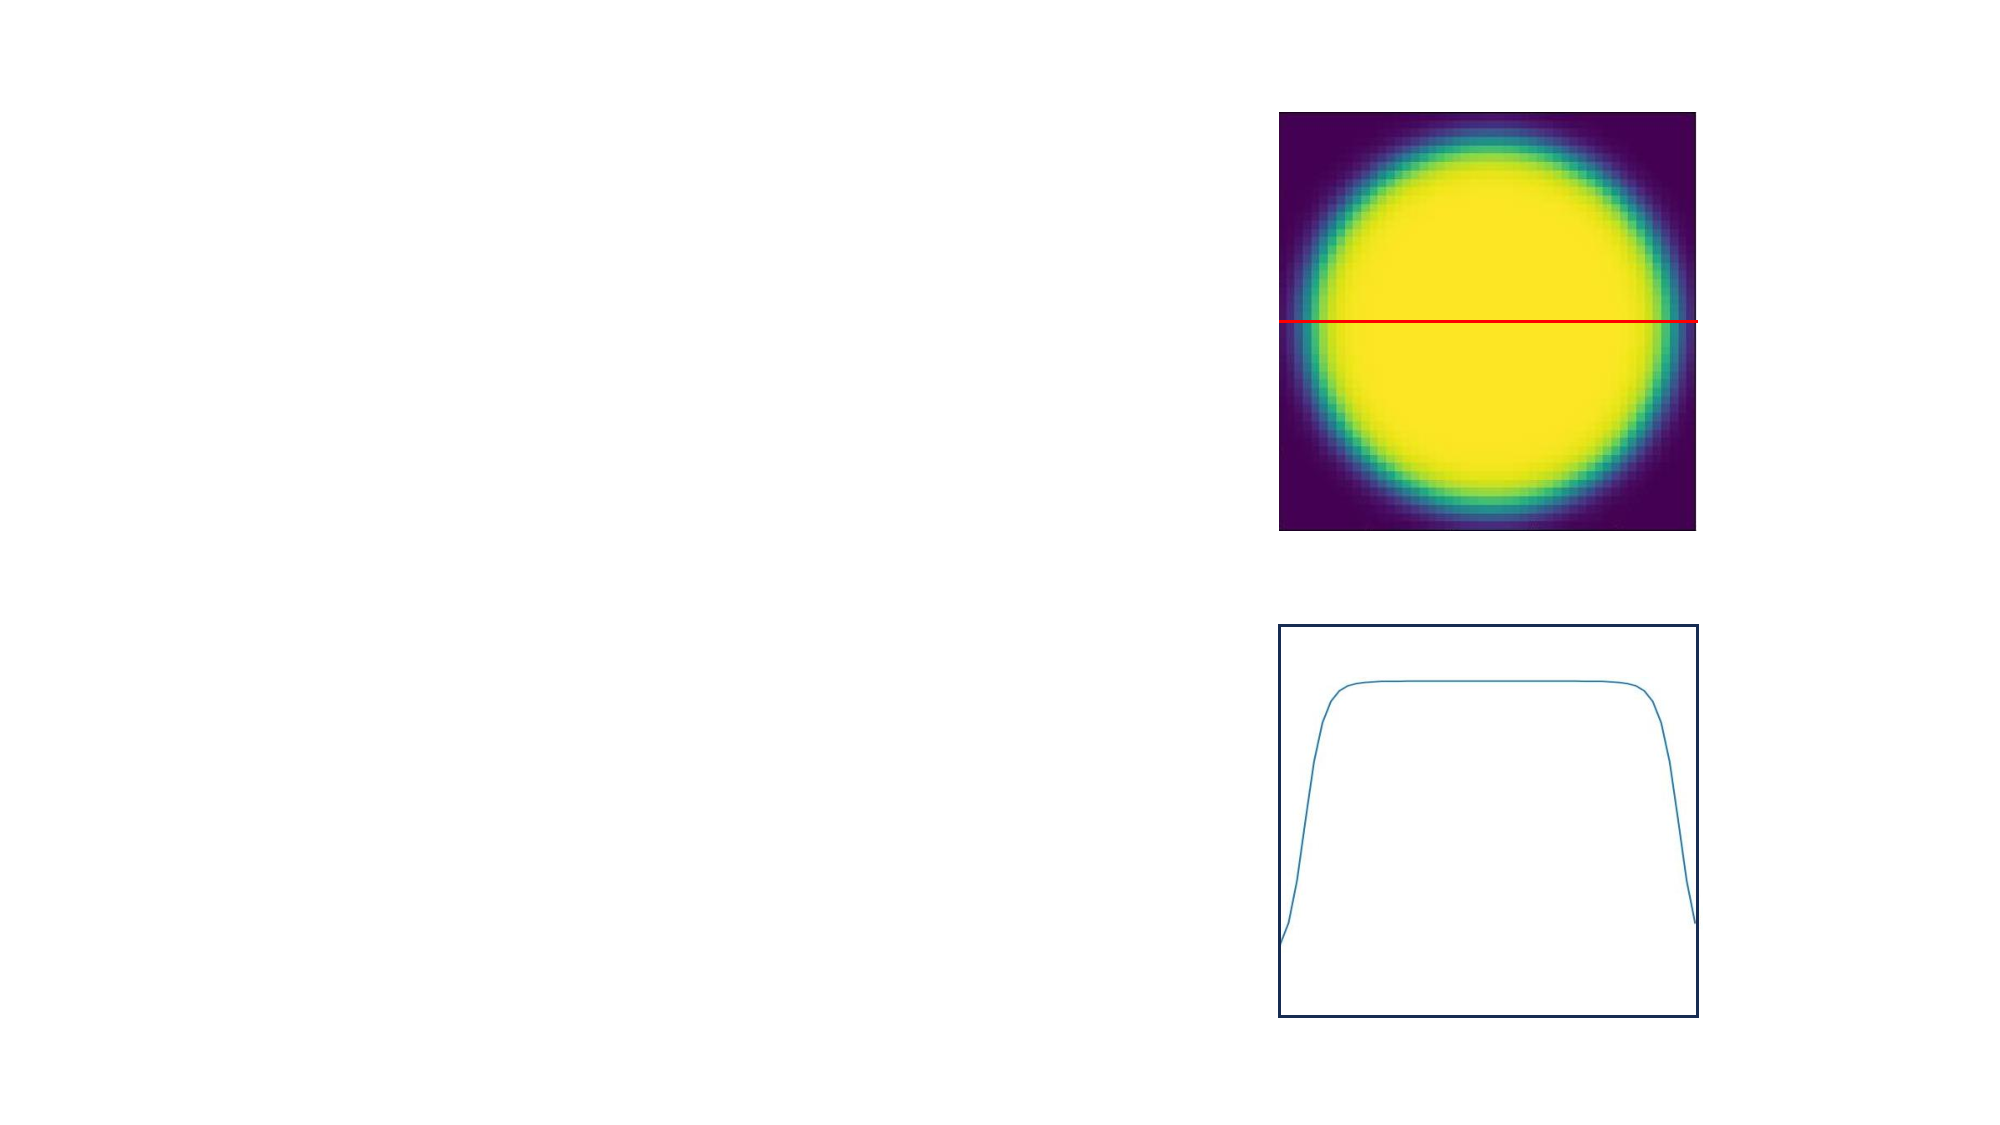
\includegraphics[height=9cm]{figures/temp_distribution_c_1.pdf}
        \caption{Sigmoid}
        \label{fig: sigmoid_distribution}        
    \end{subfigure}
    \caption{Temperature field of 3 different temperature distribution and the 
    temperature profile in the middle line of the observation area. (\subref{fig: linear_distribution}): 
    Linear distribution. (\subref{fig: gaussian_distribution}): Gaussian distribution. 
    (\subref{fig: sigmoid_distribution}): sigmoid distribution}
    \label{fig: temperature_profile}
\end{figure}


Fig.\ref{fig: temperature_profile} shows three different temperature distribution 
which are able to be generated by the virtual experiment platform. Namely linear 
distribution, gaussian distribution and sigmoid distribution. In order to simplify 
the visualization process, all temperature fields are generated based on the center 
point of the observation area. As the temperature of each point is calculated 
based on the normalized distance $d_{rel}$ or absolute distance ${d_{abs}}$ to the center point of the observation area.


Linear distribution means that the temperature increases linearly from the back ground 
area to the center point of the observation area. The details can be found in 
Eq.\ref{eq: linear_distribution}. This distribution has the potential to 
demonstrate the spectral radiation behavior of the hypothetical material in 
different temperature. 


\begin{equation}
    t = t_{center} + (t_{background} - t_{center}) \cdot d_{rel}
    \label{eq: linear_distribution}
\end{equation}


Gaussian distribution is also called normal distribution. In this distribution 
type, the temperature field in observation area obeys gaussian distribution described 
in Eq.\ref{eq: gaussian_distribution}. With the temperature of the center 
point in observation area equals the defined center temperature. Due to energy input 
of the system and heat transfer in metal powder, this temperature distribution 
is more likely to simulate the real situation in experiment.

\begin{equation}
    t = t_{center} + (t_{background} - t_{center}) \cdot \exp {\left(-\frac{d_{abs}}{2 \cdot \sigma^2}\right)}
    \label{eq: gaussian_distribution}
\end{equation}


Different to the temperature field mentioned before, the temperature in the center region 
of observation area remains constant. The mathematical expression can be found in 
Eq.\ref{eq: sigmoid_distribution}:

\begin{equation}
    t = t_{center} + (t_{background} - t_{center}) \cdot \sigmoid\left( \left(\frac{d_{abs}^2}{r_{set}^2} + 1\right)\cdot 1000\right)
    \label{eq: sigmoid_distribution}
\end{equation}


With sigmoid function can be found in Eq.\ref{eq: sigmoid_function}:

\begin{equation}
    \sigmoid(x) = \left(1 + \exp\left(-\frac{x}{100}\right)\right)
    \label{eq: sigmoid_function}
\end{equation}


Sigmoid function gaves the opportunity to perform the temperature estimation algorithm 
in a stable temperature. Thus, the potential to investigate the consistency of the 
temperature estimation algorithm and performance of the noise cancellation program is 
given. 


\subsection{Emissivity model}%
Obtaining temperature field of the hypothetical material, an emissivity model 
is required to calculate the physical value of spectral radiation intensity 
emitted from the hypothetical material.


\begin{figure}[htbp]
    \centering
    \begin{subfigure}{0.3\linewidth}
      \centering
      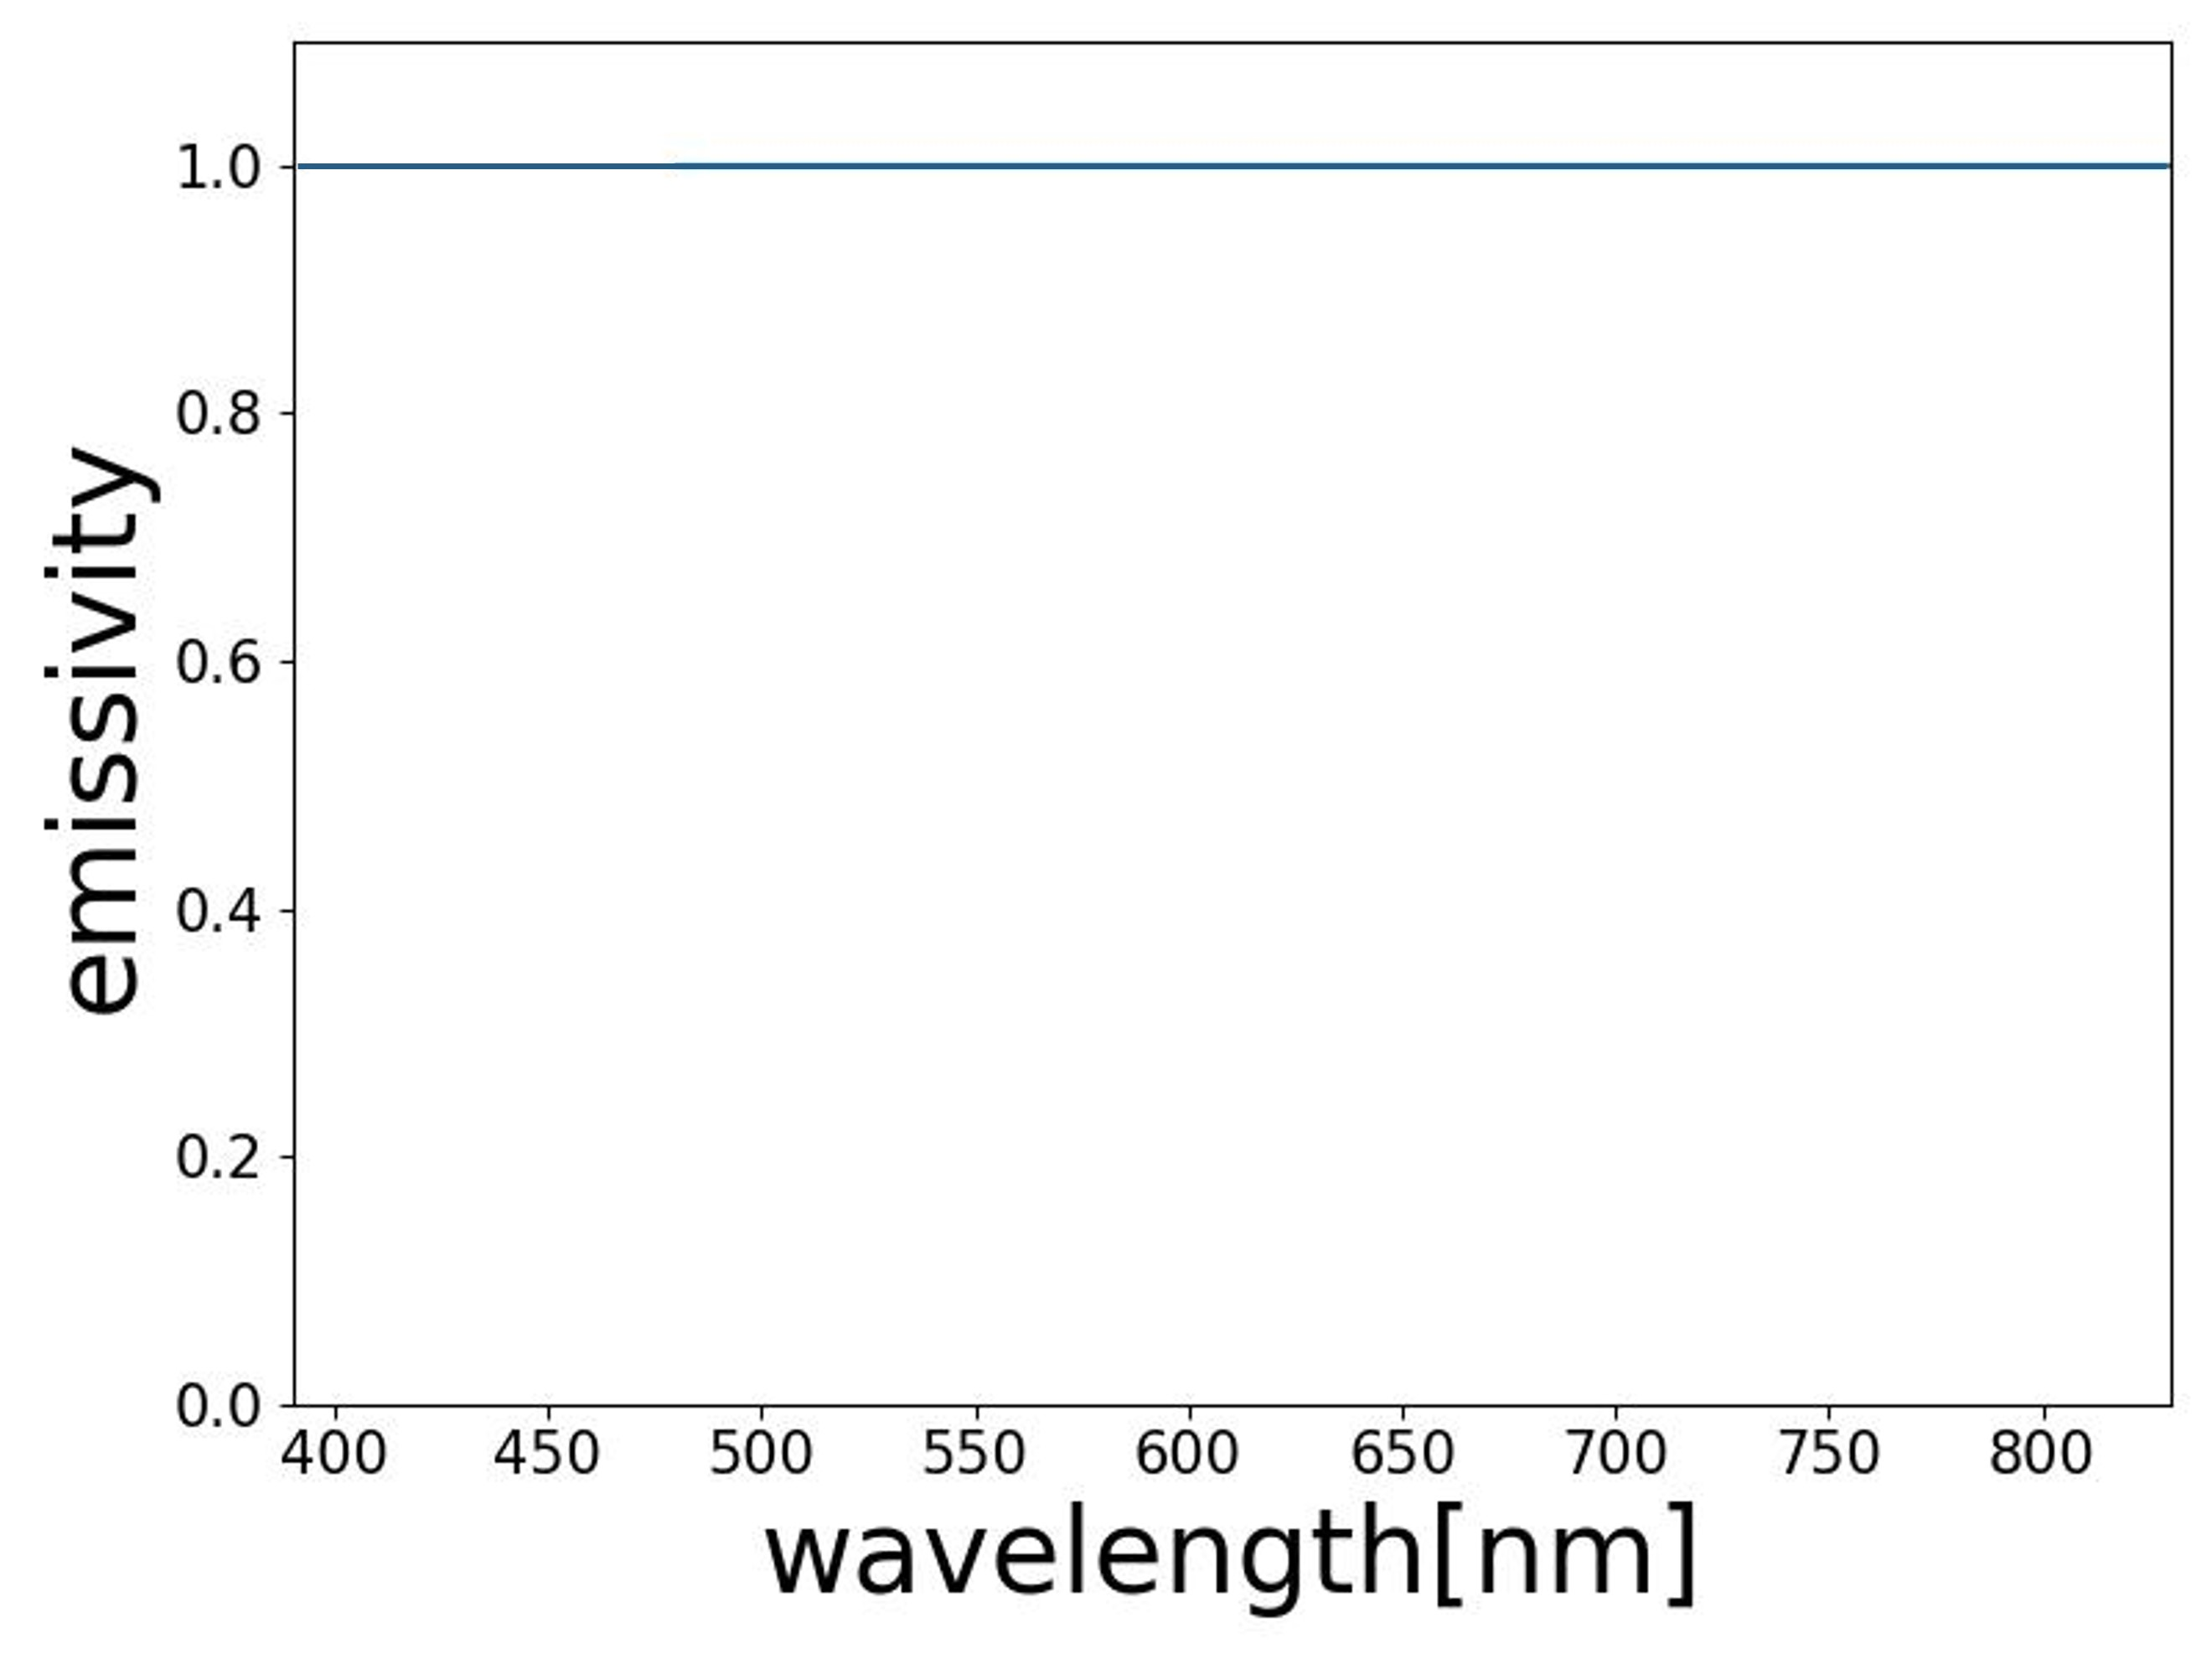
\includegraphics[width=\linewidth]{figures/emissivity_0.jpg}
      \caption{Black body model}
      \label{fig: emi_0}
    \end{subfigure}
    \hfill
    \begin{subfigure}{0.3\linewidth}
      \centering
      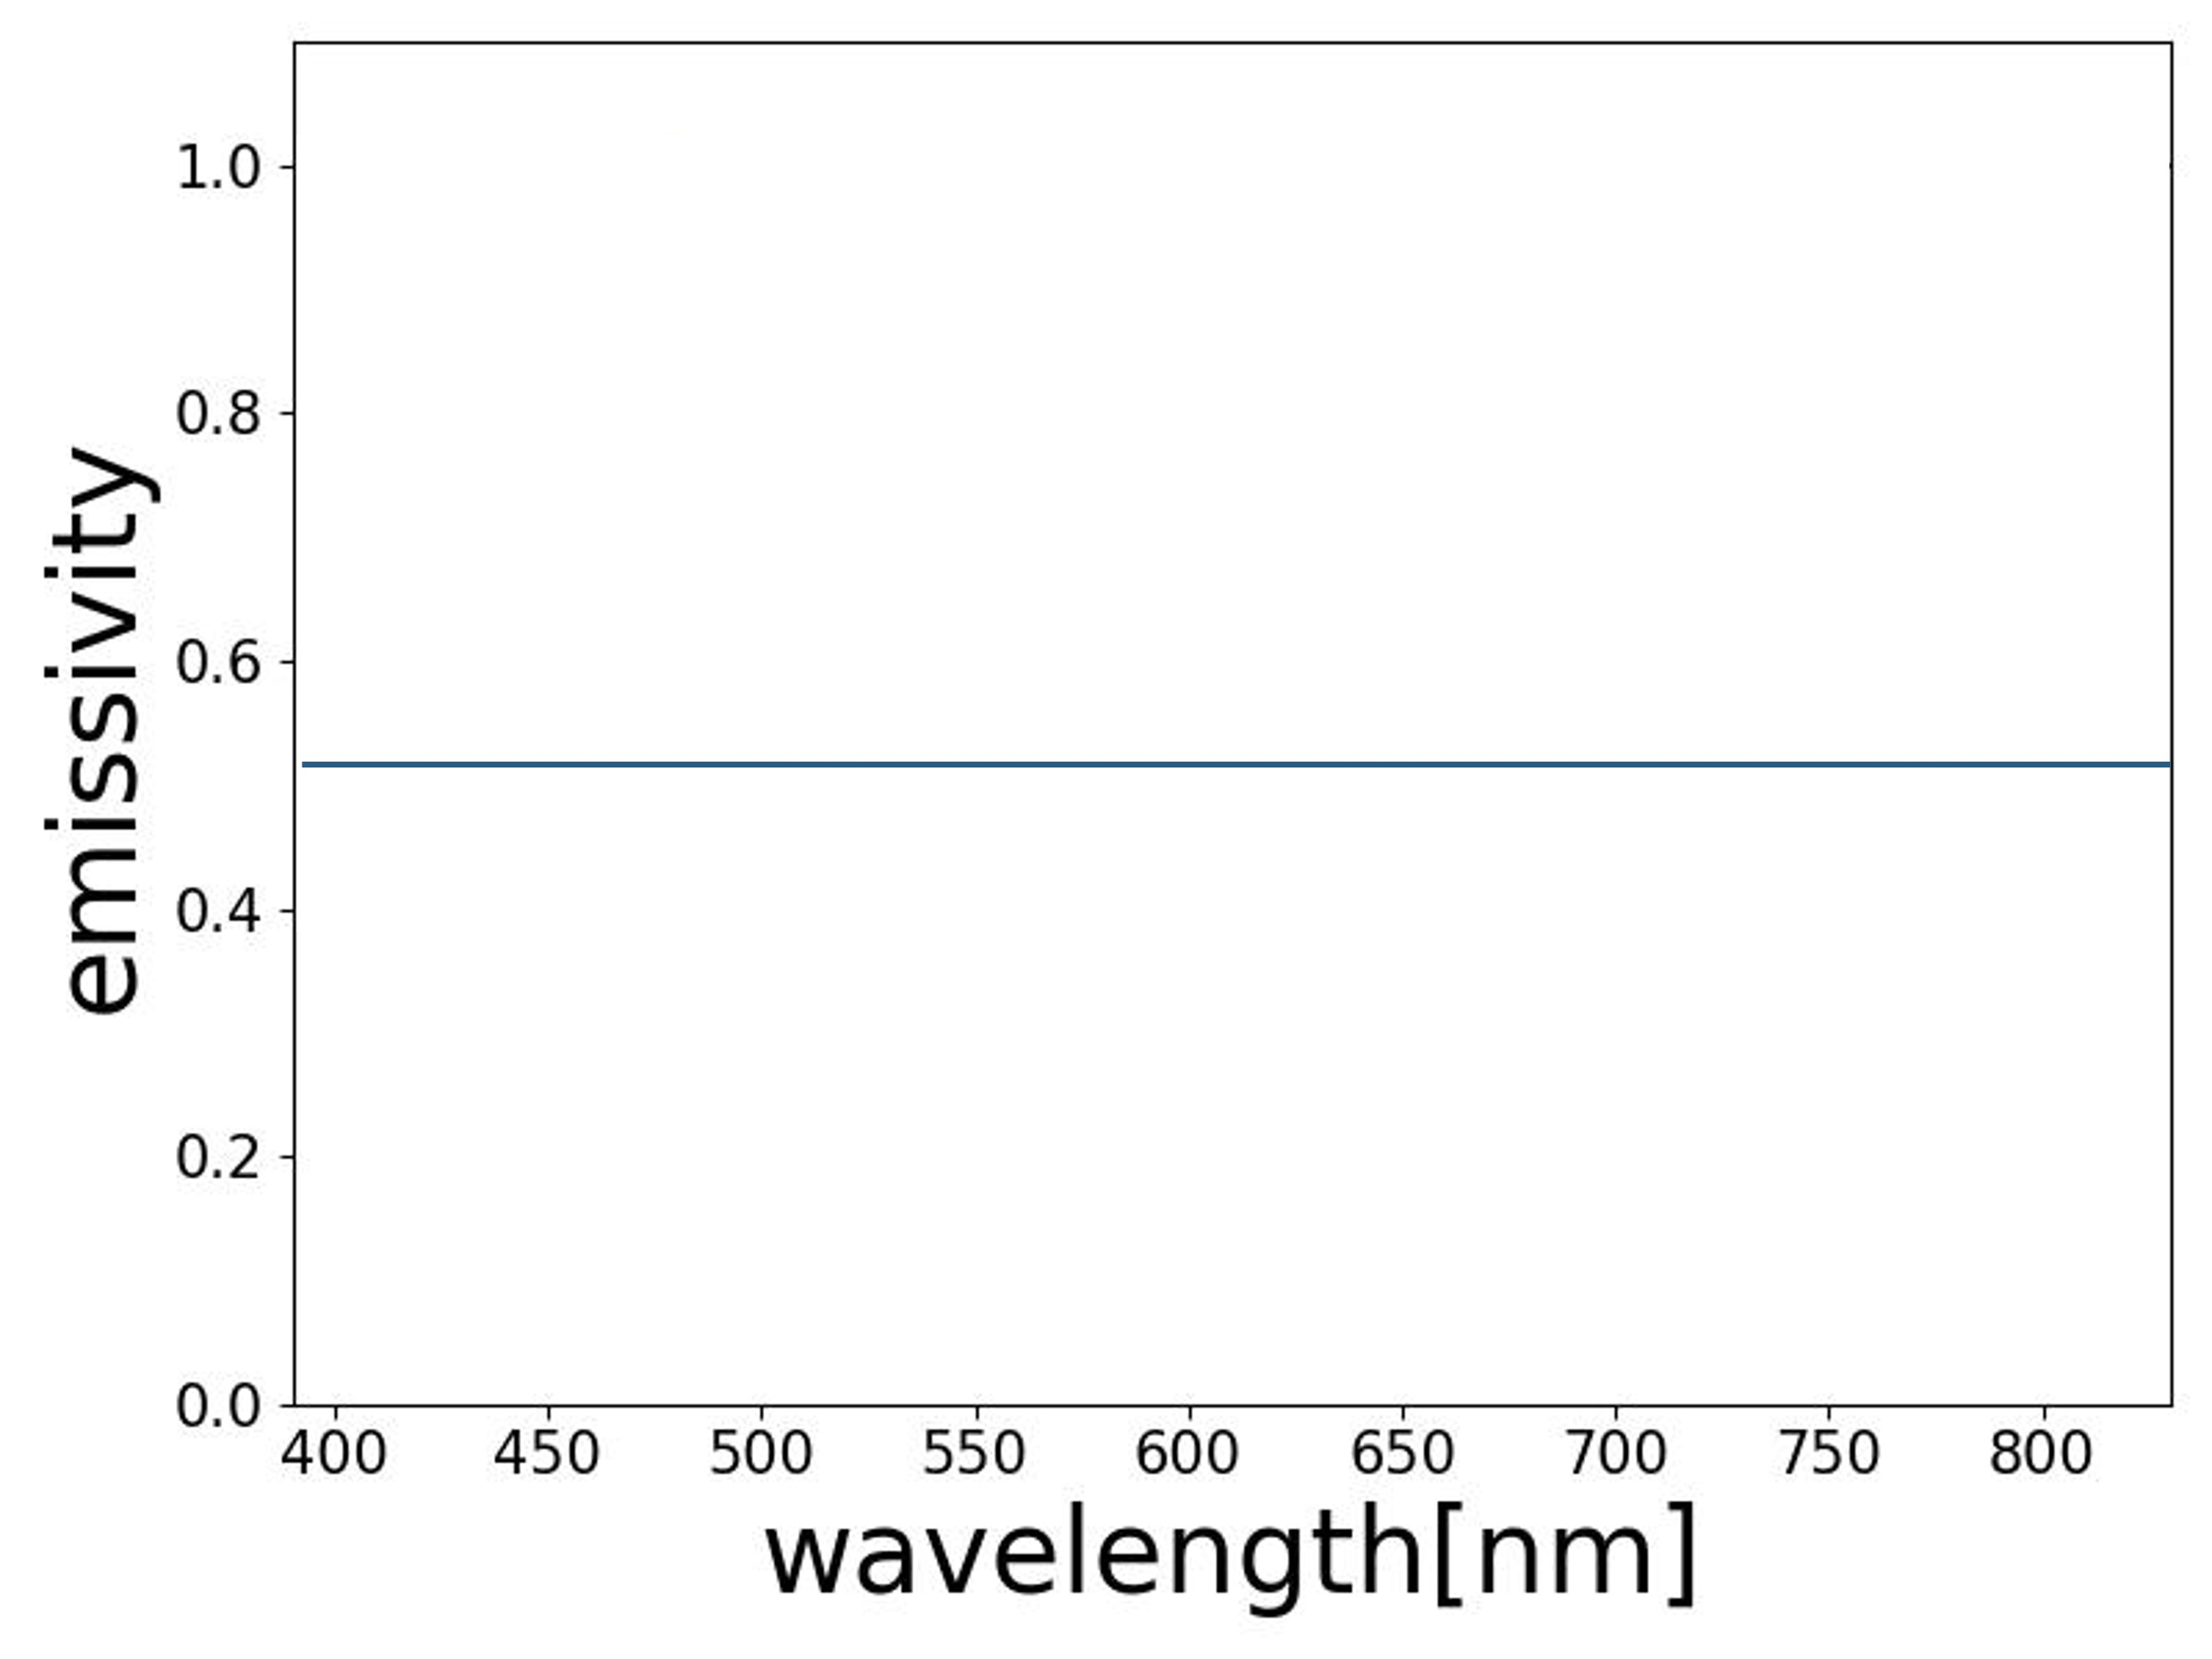
\includegraphics[width=\linewidth]{figures/emissivity_1.jpg}
      \caption{Gray body model}
      \label{fig: emi_1}
    \end{subfigure}
    \hfill
    \begin{subfigure}{0.3\linewidth}
      \centering
      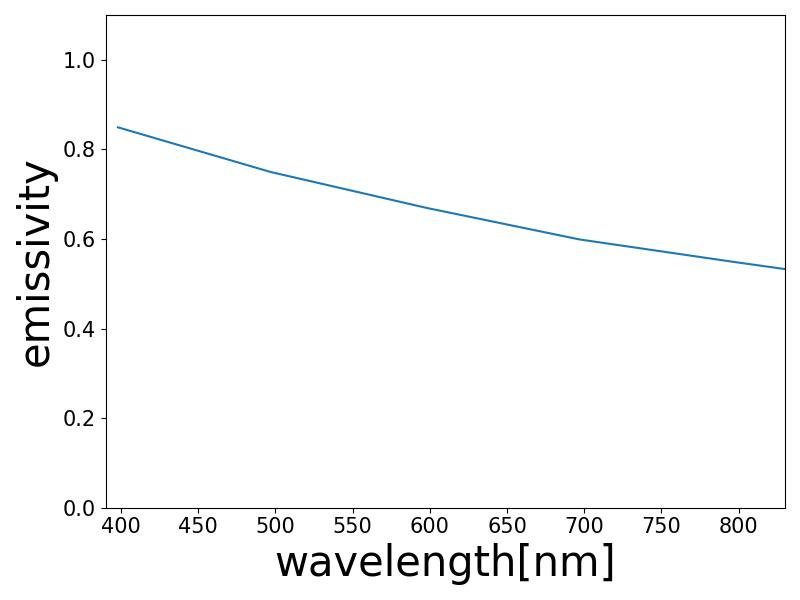
\includegraphics[width=\linewidth]{figures/emissivity_21.jpg}
      \caption{Model 1}
      \label{fig: emi_21}
    \end{subfigure}
    
    \medskip
    
    \begin{subfigure}{0.3\linewidth}
      \centering
      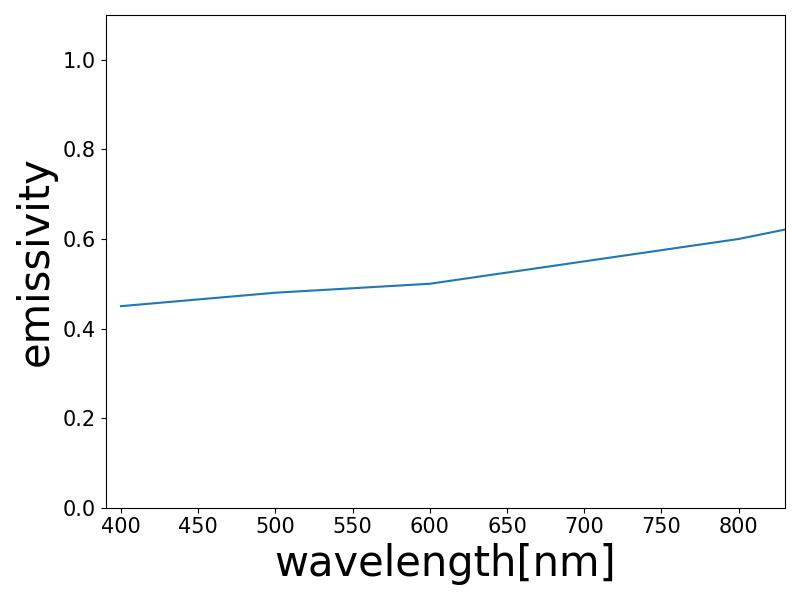
\includegraphics[width=\linewidth]{figures/emissivity_22.jpg}
      \caption{Model 2}
      \label{fig: emi_22}
    \end{subfigure}
    \hfill
    \begin{subfigure}{0.3\linewidth}
      \centering
      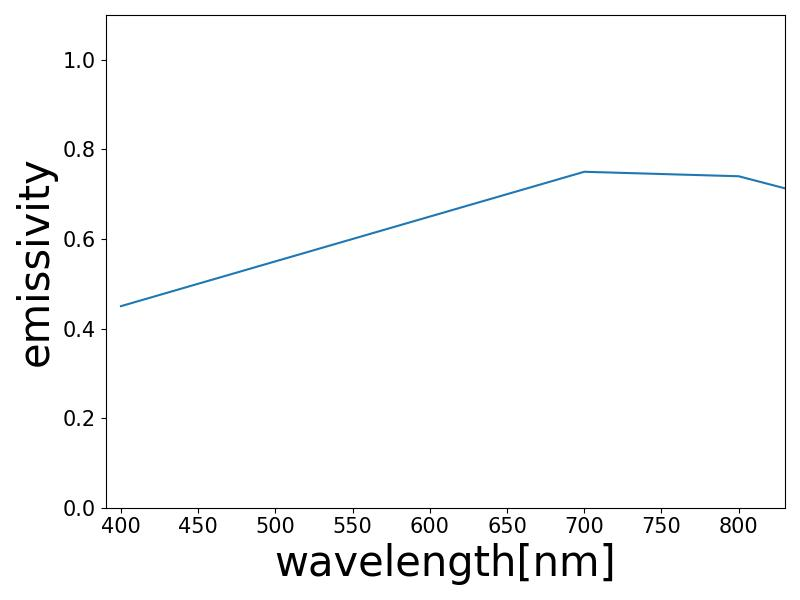
\includegraphics[width=\linewidth]{figures/emissivity_23.jpg}
      \caption{Model 3}
      \label{fig: emi_23}
    \end{subfigure}
    \hfill
    \begin{subfigure}{0.3\linewidth}
      \centering
      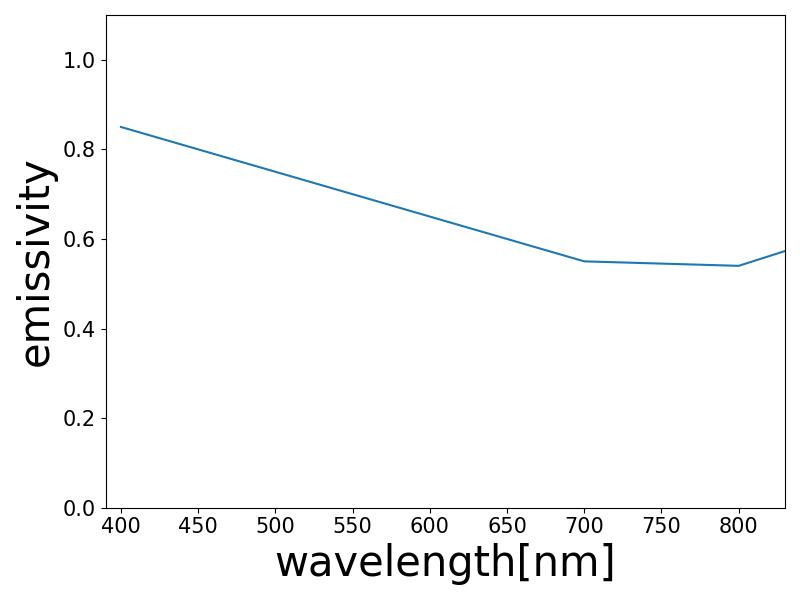
\includegraphics[width=\linewidth]{figures/emissivity_24.jpg}
      \caption{Model 4}
      \label{fig: emi_24}
    \end{subfigure}
    
    \medskip
    
    \begin{subfigure}{0.3\linewidth}
      \centering
      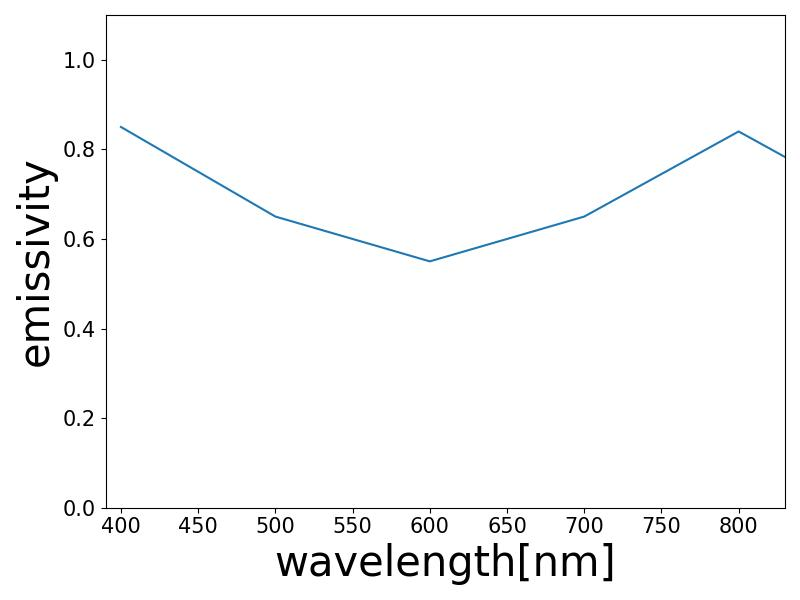
\includegraphics[width=\linewidth]{figures/emissivity_25.jpg}
      \caption{Model 5}
      \label{fig: emi_25}
    \end{subfigure}
    \hfill
    \begin{subfigure}{0.3\linewidth}
      \centering
      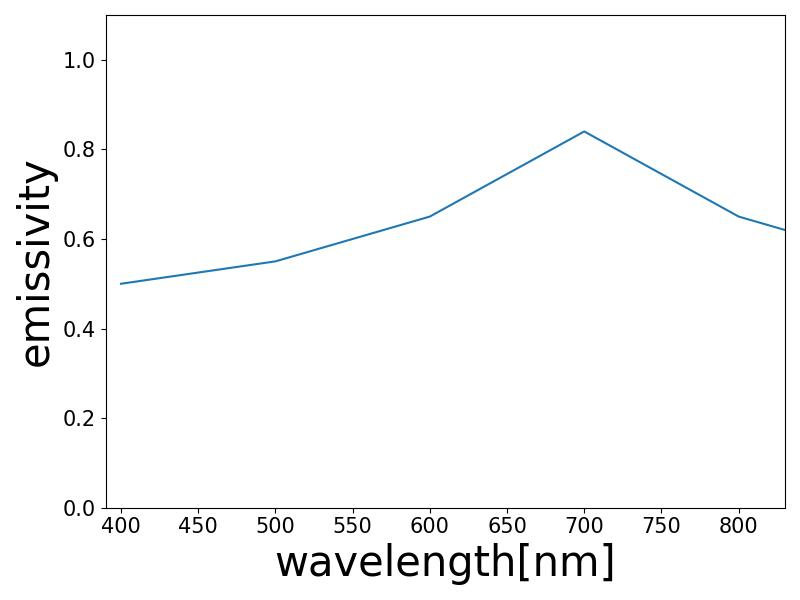
\includegraphics[width=\linewidth]{figures/emissivity_26.jpg}
      \caption{Model 6}
      \label{fig: emi_26}
    \end{subfigure}
    \hfill
    \begin{subfigure}{0.3\linewidth}
      \centering
      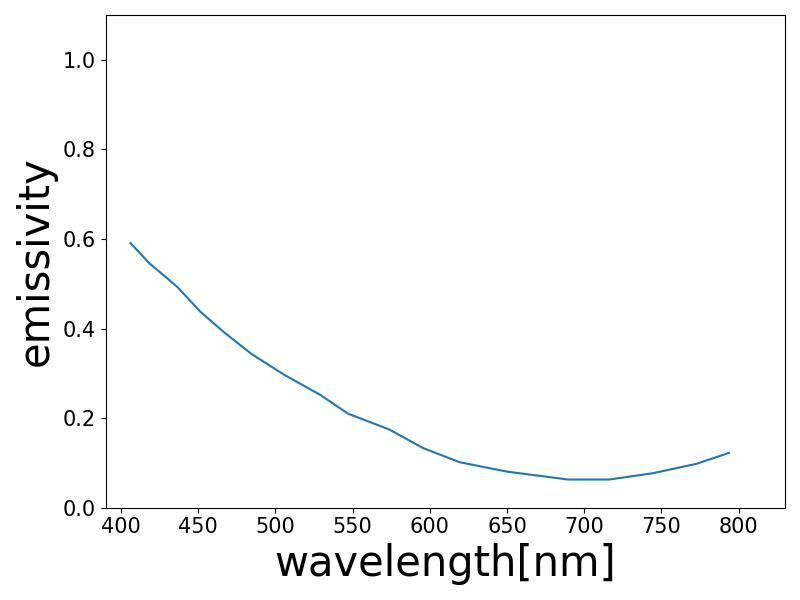
\includegraphics[width=\linewidth]{figures/emissivity_31.jpg}
      \caption{Model 7}
      \label{fig: emi_31}
    \end{subfigure}
    
    \medskip
    
    \begin{subfigure}{0.3\linewidth}
      \centering
      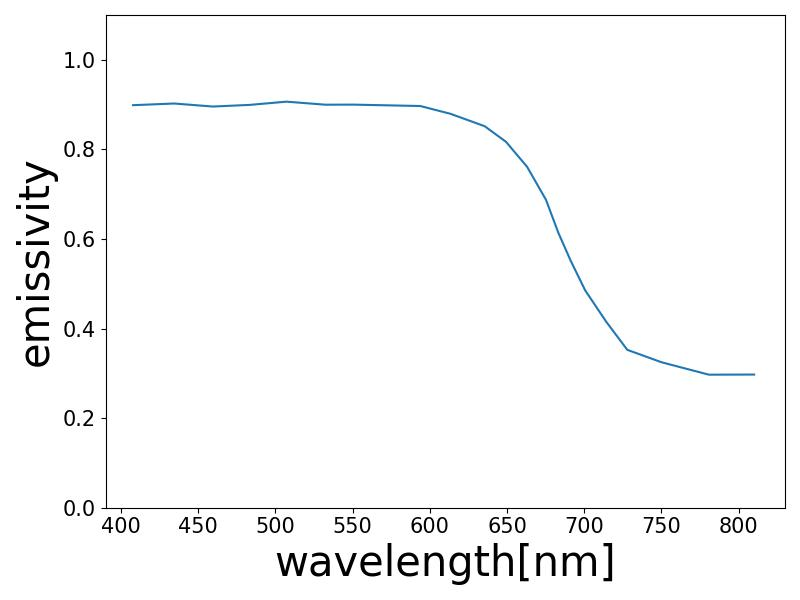
\includegraphics[width=\linewidth]{figures/emissivity_32.jpg}
      \caption{Model 8}
      \label{fig: emi_32}
    \end{subfigure}
    \hfill
    \begin{subfigure}{0.3\linewidth}
      \centering
      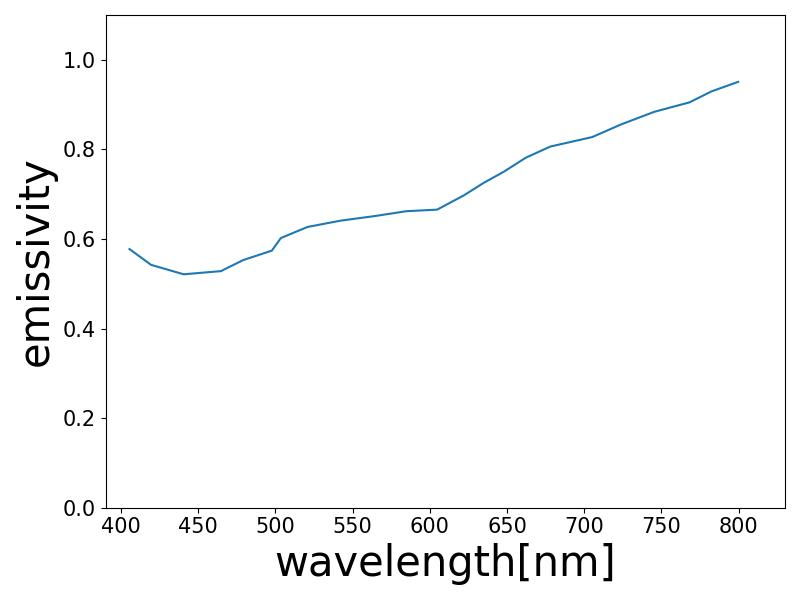
\includegraphics[width=\linewidth]{figures/emissivity_33.jpg}
      \caption{Model 9}
      \label{fig: emi_33}
    \end{subfigure}
    \hfill
    \begin{subfigure}{0.3\linewidth}
      \centering
      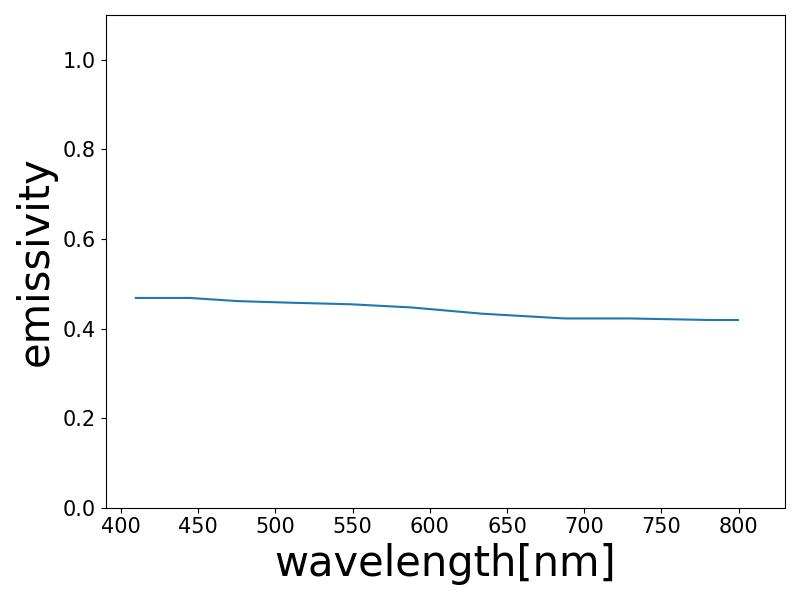
\includegraphics[width=\linewidth]{figures/emissivity_34.jpg}
      \caption{Model 10}
      \label{fig: emi_34}
    \end{subfigure}
    
    \caption{Raw emissivity data used in virtual experiment platform. (\subref{fig: emi_0}), 
    (\subref{fig: emi_1}) are black body and gray body; (\subref{fig: emi_21}) - (\subref{fig: emi_26})
    are hypothetical materials\cite{Wang.2021b}; (\subref{fig: emi_31}) - 
    (\subref{fig: emi_34}) are real materials\cite{Taunay.2020b}.}
    \label{fig: emi_model}
\end{figure}


Since the emissivity of metal powder is wavelength ($\lambda$) and temperature 
($T$) relevant, the emissivity model in this virtual experiment platform is 
formed based on the Eq.\ref{eq: emissivity}. 


\begin{equation}
  \label{eq: emissivity}
  \varepsilon(\lambda, T) = \varepsilon _{raw}(\lambda) \cdot K_T(T)
\end{equation}


The raw emissivity data $\varepsilon_{raw}(\lambda)$ in Fig.\ref{fig: emi_model}
are obtained by Wang et al.\cite{Wang.2021b} and Taunay et 
al.\cite{Taunay.2020b}. These data sets could be used to simulate the 
radiation behavior of various hypothetical materials.


After obtaining the raw data on the relationship between emissivity 
and wavelength, the dependence of emissivity on temperature is characterised
as a temperature factor $K_T(T)$ in Eq.\ref{eq: k_t}.

\begin{equation}
  \label{eq: k_t}
  K_T(T)=\begin{cases}
    1 - T_{ref} \cdot 0.2 &   T<T_{melt}\\
    \left(1 - T_{ref} \cdot 0.2 \right) \cdot 0.1 &  T\geq T_{melt}
  \end{cases}
\end{equation}


With 

\begin{equation}
  \label{eq: t_ref}
  T_{ref}=\frac{T - T_{lb}}{T_{ub} - T_{lb}}
\end{equation}


This temperature factor describes the tendency 
of emissivity to decrease with increasing temperature between $T_{lb}$ and $T_{ub}$, 
on the other hand, it also describes the change of emissivity due to the 
phase change of the hypothetical material that occurs at melting 
temperature $T_{melt}$.

\begin{figure}[htbp]
  \centering
  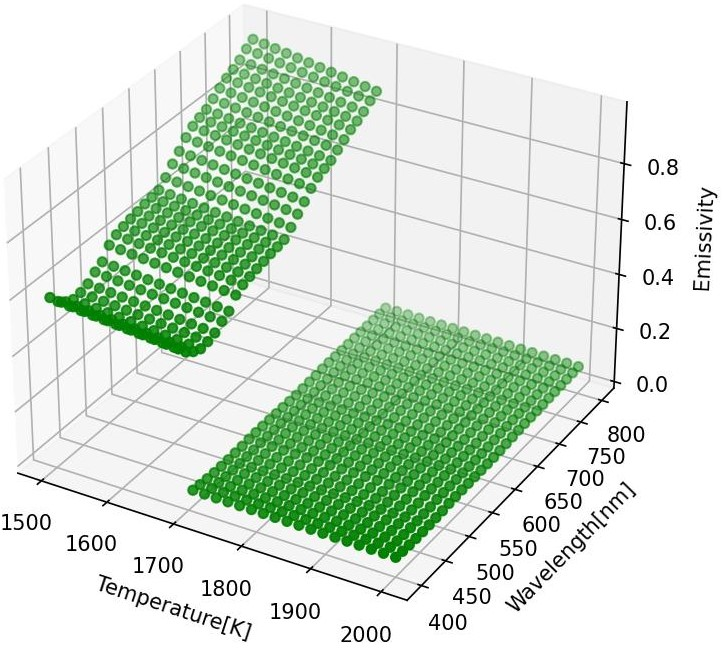
\includegraphics[width=0.6\textwidth]{figures/emissivity_model.jpg}
  \caption{Emissivity value along wavelength and temperature calculated from model 9}
  \label{fig: emissivity_model}
\end{figure}


Fig.\ref{fig: emissivity_model} shows the emissivity model based 
on model 9 in different temperature 
and wavelength. It can be found that the emissivity at a temperature 
below melting temperature ($1700K$) varies significantly with wavelength.
This is caused due to the raw emissivity data. Then, at liquid phase of 
the hypothetical material, emissivity decreases to a value lower than $0.1$.


Thus, the phase change phenomenon of hypothetical material is also characterized, 
which gives the virtual experiment platform more potential to simulate 
real experiments.


\subsection{Camera model}
After obtaining the temperature field and emissivity model of hypothetical material, 
the physical value of spectral radiation intensity should be calculated, then, 
the physical value of spectral radiation intensity is converted to 
digital value using camera model, which is the output of the complete virtual 
experiment platform. 


To ensure consistency and scalability within the program for future feature 
additions, all calculations in the program are conducted using metric units. 
For instance, temperature is measured in Kelvin, and wavelength is measured in 
meters. Therefore, it is crucial to note that the unit of wavelength in the camera 
model's calculations is meters, not nanometers. This ensures dimensional 
correctness throughout the integration process.


As mentioned in Fig.\ref{fig: received}, the camera model is based on an integration 
method, which integrate the spectral intensity received by the sensor along the 
specific range of wavelength. However, due to the varying quantum 
efficiency of each channel in sensor, it means that for a virtual camera 
with 8 channels, each pixel requires 8 independent integration operations. 
This operation requires a large computational effort. So, in order to 
accelerate the generation speed and thus reduce the time cost of virtual 
experiment platform, a parallel computing strategy is introduced.


\begin{figure}[htbp]
  \centering
  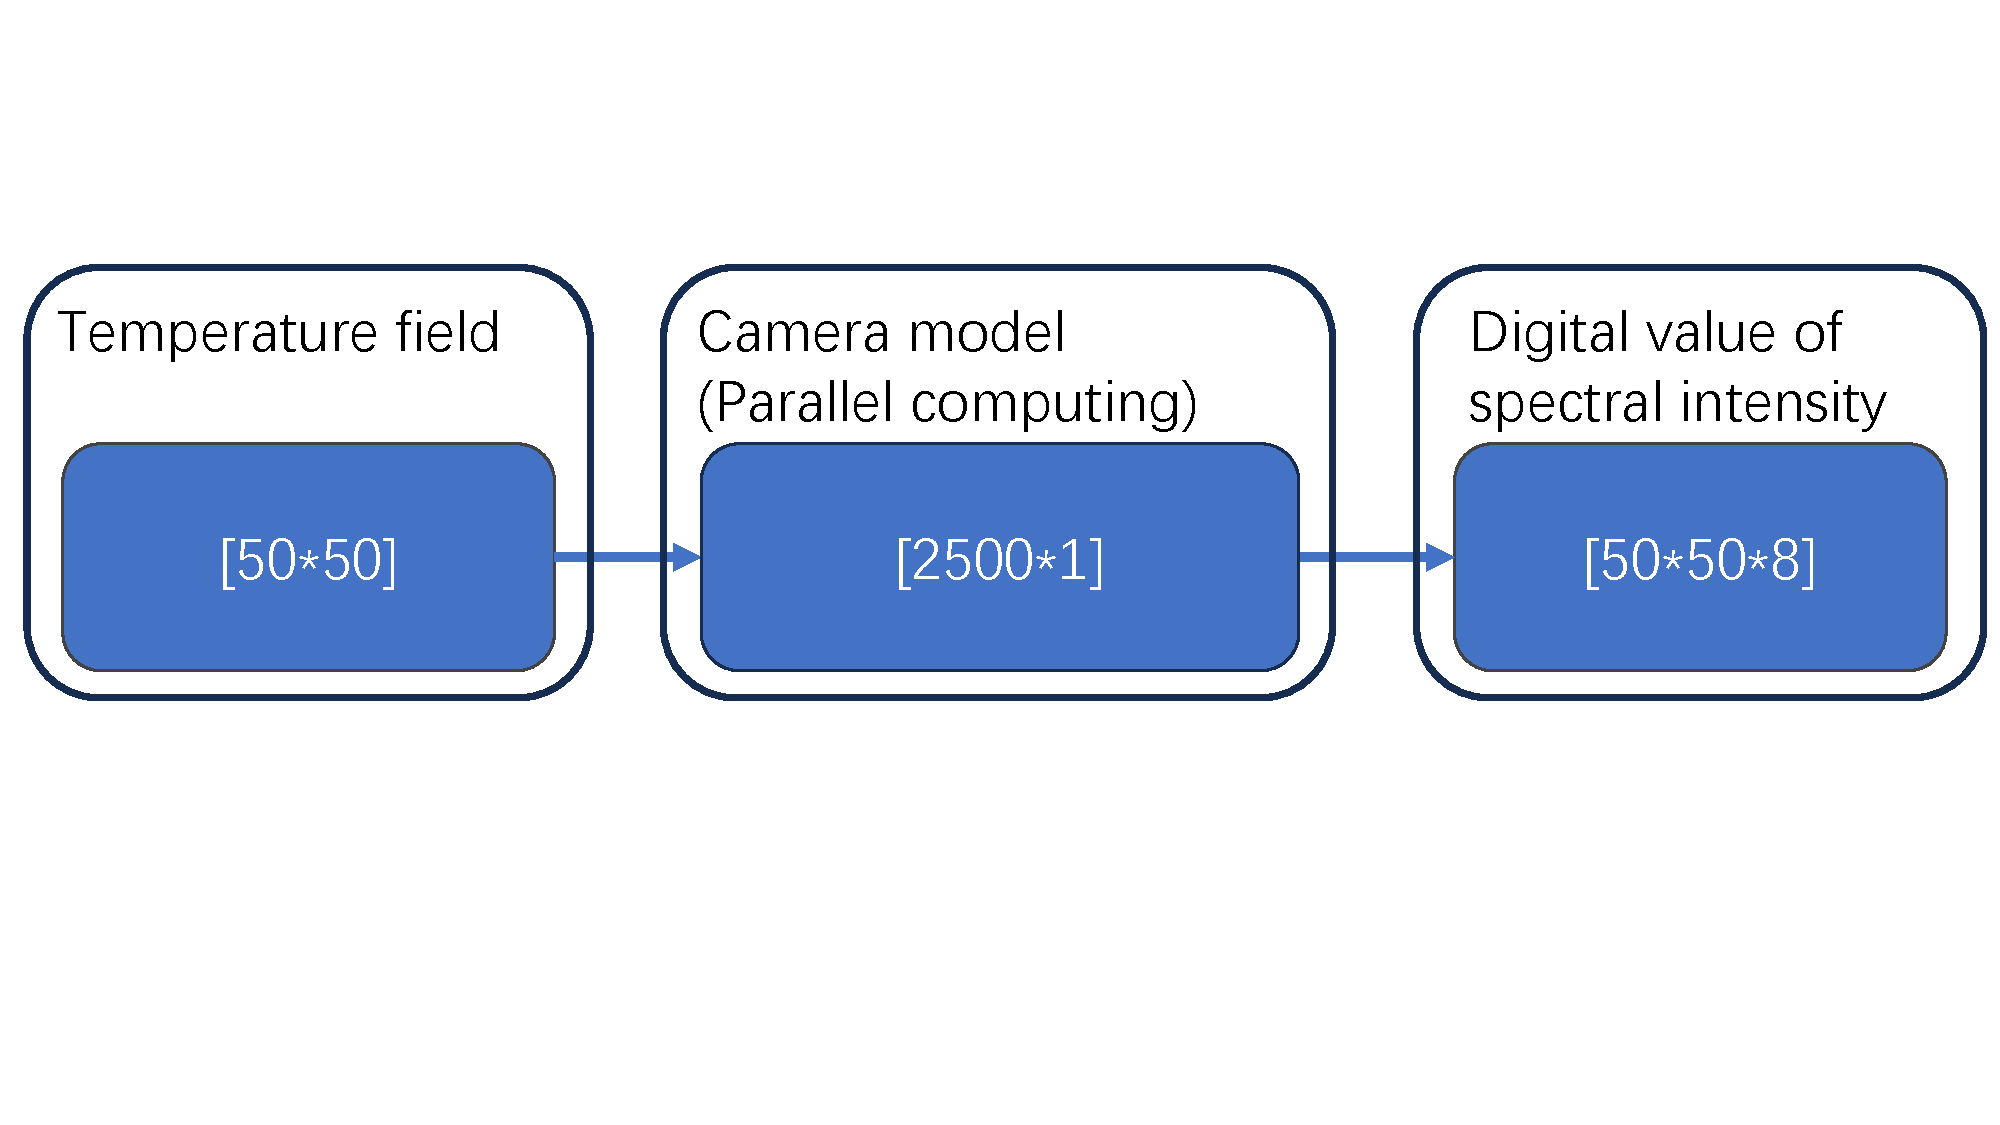
\includegraphics[width=0.9\textwidth]{figures/reshape.pdf}
  \label{fig: reshape}
  \caption{Shape of array used in camera model}
\end{figure}


The essence of parallel computing lies in decomposing a complex task into 
multiple tasks and utilizing multithreading techniques to execute these 
computational tasks simultaneously on different cores of the CPU. In 
this context, the camera model treats the integral computation on each pixel as an 
individual task, thereby significantly improving CPU utilization and substantially 
reducing computational time\cite{Asanovic.2009}. To facilitate task partitioning, the 
dimension of the temperature field 
mentioned earlier in this section needs to be reduced, from 
a $50\times 50$ matrix to a one-dimensional array of size $2500\times1$. This allows for 
obtaining 2500 parallel tasks. Once the calculations are completed, the 
resulting matrix of size $2500\times8$ is then transformed back into a three-dimensional 
matrix of size $50\times50\times8$. In this manner, a digital value similar to the data 
obtained in real experiments is computed.


\section{Temperature estimation algorithm}
After obtaining the digital value of spectral radiation intensity, 
the tasks of this virtual experiment platform are considered complete, 
and the next step involves data processing and calculations. The core 
of the temperature estimation algorithm lies in reconstructing the physical 
value of spectral radiation intensity based on the known digital values and 
the choosen parameters. 
Subsequently, through the implementation of a curve fitting algorithm, the 
estimated emissivity and temperature can be calculated.


\subsection{Rebuild physical value of spectral radiation intensity}
Hence, it is evident that the process of reconstructing the physical value holds 
significant importance in the temperature estimation algorithm. This reconstruction 
process represents the conversion of spectal radiation intensity from its physical value to a 
digital value. By analyzing the reconstructed results, the 
relationship between the physical value $(I_{rec})$ and the parameters $(T, k)$ to be fitted can be established, 
where $T$ and $k$ are derived from Eq.\ref{eq: reconstruct_integration}. Subsequently, 
by performing curve 
fit algorithm between the reconstructed physical value and the experimental data, we 
can obtain the parameters $(T, k)$ that best fit the real data. Therefore, it 
becomes apparent that the reconstruction of the physical value can affect 
the accuracy of the temperature prediction algorithm discussed in this thesis.


As mentioned in Eq.\ref{eq: reconstruct_integration}, the reconstructed physical value 
of spectral radiation intensity is generated based on the integration method. It can 
be observed that the digital value can be considered as a function of temperature of 
hypothetical material $T$ and parameters of emissivity model $k$.


\begin{equation}
  \label{eq: reconstruct_digital_value_function}
  I_{rec}^i (k, T) = q \int B(\lambda, T) \cdot \varepsilon(\lambda, k, T) 
  \cdot \eta_{camera}^i d\lambda
\end{equation}


Eq.\ref{eq: reconstruct_digital_value_function} shows the mathematical expression 
of reconstructed physical value of spectral radiation intensity of $i_{th}$ channel.
So, the current objective is to minimize the cost in Eq.\ref{eq: reconstruct_optimization} 
by optimizing the values of $k$ and $T$. In other words, the goal is to make the 
reconstructed spectral radiation intensity $I_{rec}(k, T)$ as close as possible 
to the values obtained in virtual experiments. By minimizing the cost function, 
the temperature estimation algorithm aims to achieve a high level of accuracy 
and fidelity in calculating the temperature based on the reconstructed 
digital values.


\subsection{Emissivity model used for calculation}
In the previous section, it is evident that the temperature estimation 
algorithm is essentially performing a curve fit algorithm on the parameters of the 
emissivity model and temperature of the hypothetical material. 
Therefore, the choice of the emissivity model significantly impacts 
the accuracy of the temperature estimation algorithm. In order to 
enhance the generality of this temperature prediction algorithm and 
prevent overfitting, a hypothesis is proposed: the temperature 
prediction algorithm is unaware of the material's emissivity 
characteristics. Hence, it is necessary to use a different 
emissivity model from the one used in the virtual experiment 
platform to reconstruct the digital value of spectral radiation 
intensity.


Based on mentioned above, the temperature estimation algorithm 
introduced in this paper tested several different emissivity 
models, namely:


\begin{enumerate}
  \item Linear model
  \item Linear square model
  \item Quadratic model
  \item Exponential model
  \item A combined model composed of the linear square and exponential models
\end{enumerate}


These models are distinguished based on the relationship between 
emissivity and wavelength. Each model represents a different 
mathematical expression that describes how emissivity varies with 
wavelength. In order to simplify the calculation process and thus set 
boundary conditions of parameters $k$ in emissivity model, all wavelength 
used in this emissivity model is normalized wavelength $\lambda_{norm}$. The 
mathematical expression can be described as followed:

\begin{equation}
  \label{eq: wavelength_norm}
  \lambda_{norm} = \frac{\lambda - \lambda_{lb}}{\lambda_{ub} - \lambda_{lb}}
\end{equation}


To enhance the readability of the formula, the parameter $k$ in 
Eq.\ref{eq: reconstruct_digital_value_function} is written in vector 
form in Eq.\ref{eq: k_vec} based on the number of parameters in emissivity model.

\begin{equation}
  \label{eq: k_vec}
  k = \begin{pmatrix}
    a \\
    b \\
    c \\
    \end{pmatrix} 
    or 
    \begin{pmatrix}
      a \\
      b \\
      \end{pmatrix}
\end{equation}
With the lower boundary of wavelength $\lambda_{lb} = 500 {nm}$ and the 
upper boundary of wavelength $\lambda_{ub} = 1000 {nm}$. Thus, the input 
of the emissivity model used in temperature estimation algorithm is thus 
dimensionless number.

\subsubsection{Linear model}
Linear model refers to a linear relationship between emissivity and wavelength,
which could be written as Eq.\ref{eq: emi_lin}:

\begin{equation}
  \label{eq: emi_lin}
  \varepsilon(\lambda) = a\cdot \lambda_{norm} + b
\end{equation}

The linear model represents the simplest and most straightforward emissivity model. 
It provides an easy way to visualize the calculated emissivity model 
and reduces complexity in defining various boundary conditions within the 
emissivity model.

\subsubsection{Linear square model}
The linear square model is distinct from the linear model, 
as it incorporates three parameters representing the coefficients 
of the quadratic term, the linear term, and the constant term. Its 
mathematical expression can be described as Eq.\ref{eq: emi_lin_square}:

\begin{equation}
  \label{eq: emi_lin_square}
  \varepsilon(\lambda) = a \cdot \lambda_{norm}^2 + b \cdot \lambda_{norm} + c
\end{equation}

The linear square model can be used to describe more intricate emissivity 
models for materials. With an additional parameter compared to the 
previous linear model, it offers increased degrees of freedom for 
curve fitting, enabling a better fit to complex shapes. Nevertheless, 
the augmented complexity may also lead to a higher risk of overfitting as 
well as increase of computational demand required.

\subsubsection{Quadratic model}
Consequently, in order to simplify the computation of the linear 
square model, the quadratic model was introduced. In this model, 
the coefficient of the linear term in the original linear square 
model is set to 0. This simplification leads to a reduction in 
the number of parameters within the emissivity model. The emissivity model 
can be expressed as Eq.\ref{eq: emi_quad}

\begin{equation}
  \label{eq: emi_quad}
  \varepsilon(\lambda) = a \cdot \lambda_{norm}^2 + b
\end{equation}

\subsubsection{Exponential model}
In the exponential model, emissivity is exponentially related to wavelength. Due to 
the monotonic nature of the exponential function, this model enhances the accuracy of 
parameter estimation along the gradient descent of the cost function during curve fitting, 
thereby improving the computational efficiency. The mathematical expression can be 
expressed in Eq.\ref{eq: emi_exp}:

\begin{equation}
  \label{eq: emi_exp}
  \varepsilon(\lambda) = \exp(-a \cdot \lambda_{norm} - b)
\end{equation}

For materrials commonly used in \gls{pbflbm}, emissivity tends to decrease with 
increasing wavelength. Therefore, to reduce the range of parameters during curve 
fitting, the exponent term $a \cdot \lambda_{norm} + b$ was set as non-negative value.

\subsubsection{Mixed model}
This model is a combination of two models. In Fig.\ref{fig: emissivity_model}, it 
can be observed that the emissivity of the virtual material undergoes 
significant changes when the temperature exceeds the material's melting point, 
and the emissivity variations become smaller in the liquid phase. Therefore, when 
emissivity changes are relatively small, i.e., when the material is in the 
liquid phase, the exponential model is more suitable. On the other hand, when 
emissivity changes are more pronounced, i.e., when the material is in the solid 
phase, the linear square model is more appropriate. This approach not only 
improves the computational accuracy of the model in the solid region but also 
ensures the computational efficiency of the model in the liquid region.


In this model, the computation starts with the linear square model. The computed 
results are then filtered to identify points where the temperature exceeds 
the material's melting point. Subsequently, the exponential model is 
utilized to recompute the emissivity and temperature for those specific points. 
Finally, the results from both calculations are combined to obtain a higher 
precision outcome. However, this process demands higher computational resources. 
Consequently, it is observed that this model significantly increases the 
computational time required for temperature estimation algorithms.


\subsection{Curve fit algorithm}
After obtaining the reconstructed physical values of intensity, 
a curve fit algorithm is required to determine  
temperature and the parameters of the emissivity model that best 
align with the actual received intensity. However, in this work, both 
the data obtained from the virtual experimental platform and the data 
from real experiments are not continuous spectral intensities. 
Conversely, the input for this temperature estimation algorithm is a 
two-dimensional array with dimensions of 8x2, which can be regarded as 8 
samples of a continuous physical value.


\begin{figure}[htbp]
  \centering
  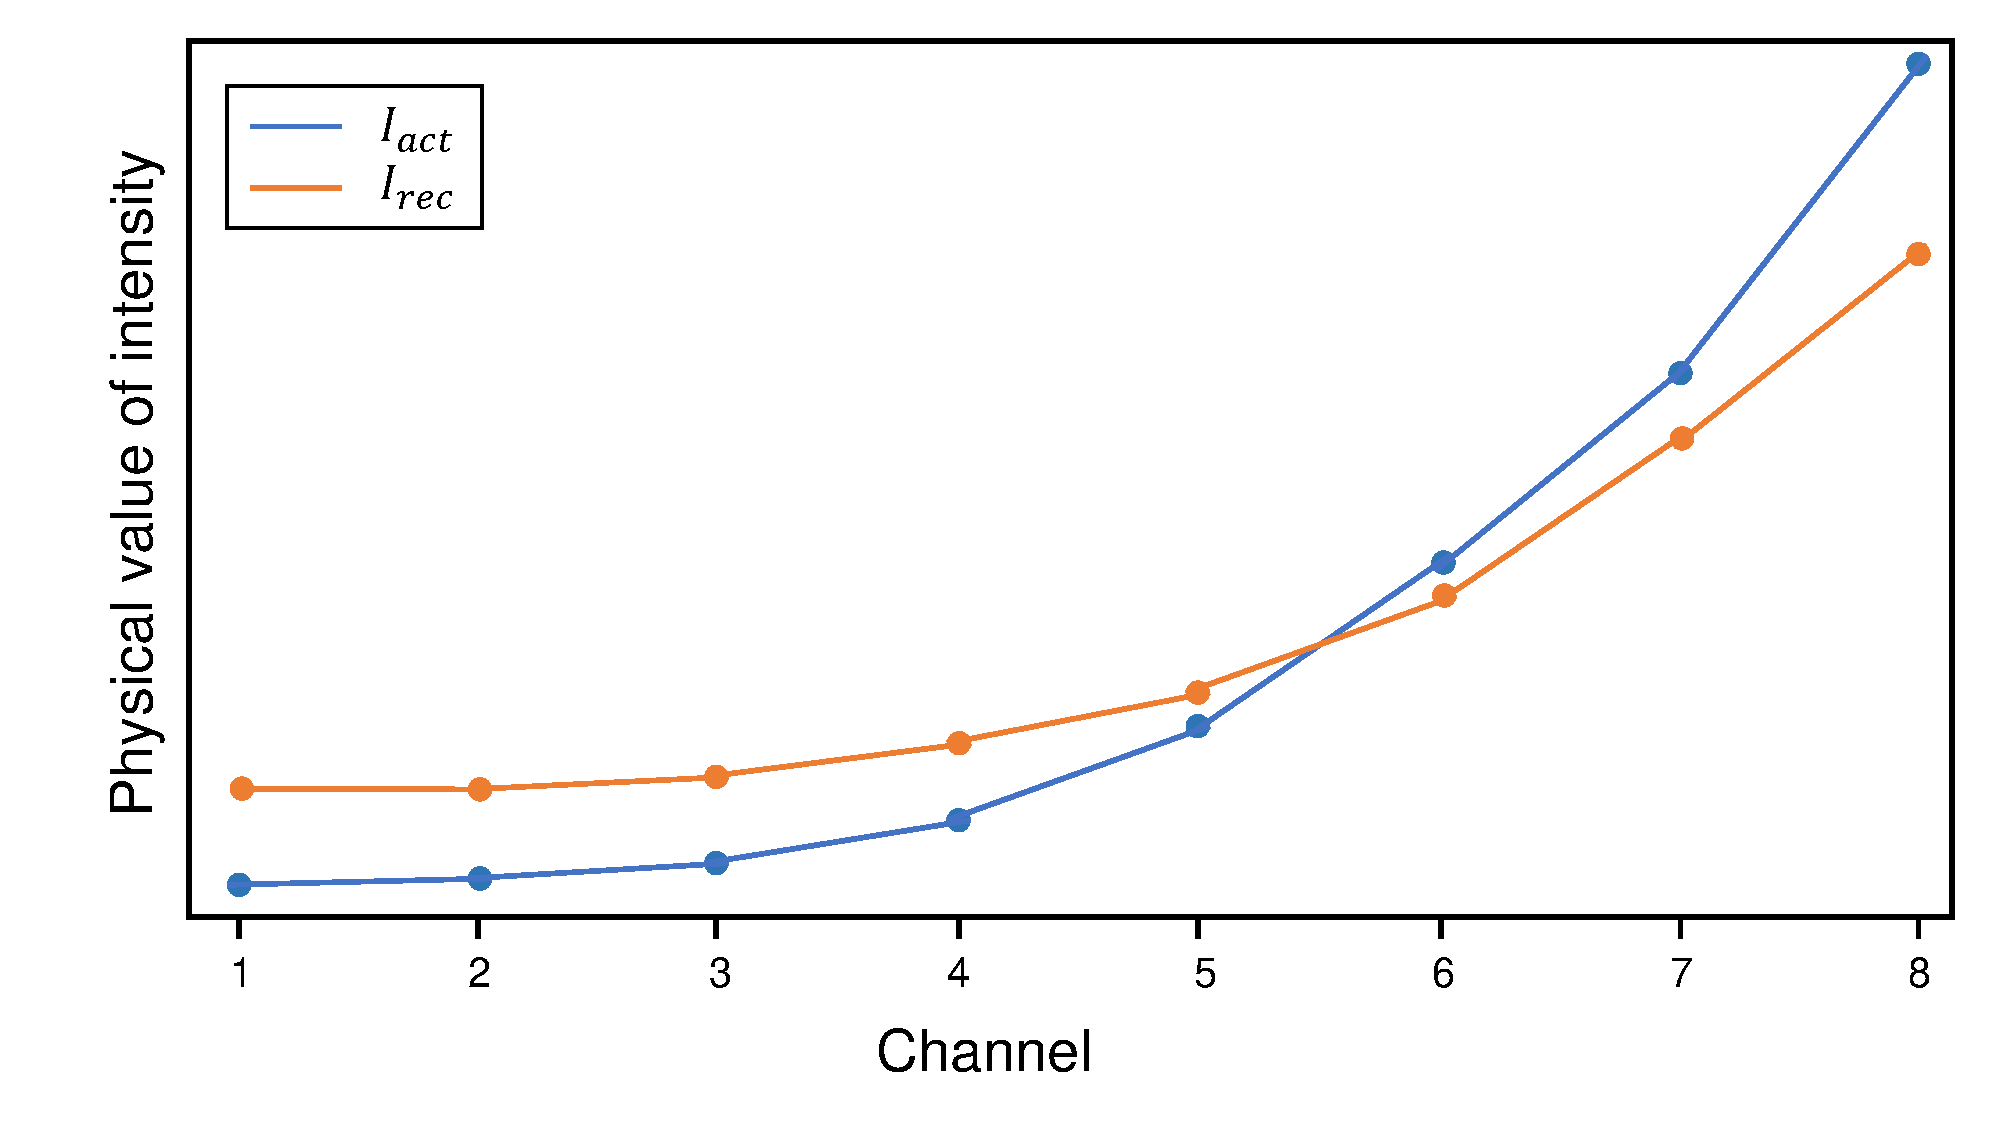
\includegraphics[width=0.9\textwidth]{figures/curve_fit.pdf}
  \caption{Comparison between actual received intensity $I_{act}$ 
  and reconstructed intensity $I_{rec}$ of one point}
  \label{fig: curve_fit_demo}
\end{figure}


Fig.\ref{fig: curve_fit_demo} illustrates the reconstructed physical 
value for each channel and the corresponding physical values from the 
original experimental data. It is evident that this approach simplifies 
the visualization of independent channel data and facilitates the 
utilization of this profile for curve fitting purposes.


\subsection{Parameters in temperature estimation algorithm}
The temperature estimation algorithm uses numerous parameters, 
which significantly impact the precision and consistency of the 
computed results. Therefore, it is essential to set boundary conditions 
for these parameters.


\subsubsection{Wavelength range}
In Fig.\ref{fig: quantum_efficiency}, it can be observed that the 
total quantum efficiency of the sensor $\eta_{camera}$ decreases to 
0 when the radiation wavelength exceeds 900 nanometers. This effect is 
attributed to the presence of a filter on the sensor. Consequently, 
when reconstructing the physical values of the spectral radiation 
intensity, the integration limits are set to be within the 
range of 500 nanometers to 1000 nanometers. This approach ensures 
that the essential information is captured while reducing the 
computational resources required for integration and thus improving the 
computational speed.


\subsubsection{Boundary condition of estimated temperature}
In the temperature estimation algorithm, the process starts with an 
initial guess, which is used to perform the first reconstruction of 
the physical values of the spectral radiation intensity. This 
reconstruction yields a cost function and a gradient that 
minimizes the cost function. The algorithm then adjusts the parameters 
to be optimized along this gradient before proceeding to the next 
iteration. It is evident that the choice of the initial guess 
significantly influences the computational efficiency of the 
program and can help avoid potential physically meaningless 
local minima.

To address this, it is mandated that the predicted temperature in the 
temperature estimation algorithm lie within the range of 500 to 2000K. 
This constraint ensures that the algorithm operates within a 
physically meaningful and relevant temperature range, preventing 
unrealistic results and potentially leading to a more effective and 
efficient optimization process.

\subsubsection{Boundary condition of estimated emissivity}
Unlike the boundary conditions applied to the estimated temperature, 
the boundaries for emissivity are much narrower. This is due to the 
physical definition of emissivity mentioned earlier in the text. 
Therefore, it is necessary to apply a boundary condition 
of $0 < \varepsilon < 1$ for emissivity during the calculations. 
However, in the curve fit algorithm mentioned in this work, emissivity 
is not a variable to be determined. Hence, it becomes necessary to 
incorporate this boundary condition directly into the emissivity model.%
\chapter{Calcualtion results and analysis}
Once all the experiment data and parameters are determined, the results 
of the calculation should be presented and analyzed. Thus, the 
accuracy, consistency, pros and cons of the virtual experiment 
platform and temperature estimation algorithm can be systematically 
analyzed.

\section{Calculation results}
In virtual experiment platform and temperature estimation algorithms, emissivity is considered as a 
function of radiation wavelength and temperature. Consequently, it varies with changes in 
temperature and radiation wavelength. This variability is advantageous for enhancing algorithm 
precision but introduces difficulties in visualizing computation results. Furthermore, 
temperature estimation algorithm doesn't directly calculate the emissivity of materials; 
instead, the algorithm optimize the parameters $k$ of the emissivity model. 
Thus, the emissivity data of each point is a function of wavelength $\lambda$ and thus
cannot be directly visualized. To address this, a simplified 
approach for visualizing emissivity is introduced, which allows for a more intuitive 
representation of emissivity without compromising the accuracy of the computational process.

\begin{equation}
    \label{eq: emi_average}
    \varepsilon_{sim} = \overline{\varepsilon(\lambda)} 
\end{equation}

Eq.\ref{eq: emi_average} presents the mathematical expression for this simplification. 
$\varepsilon_{sim}$ represents the simplified emissivity value, and $\varepsilon(\lambda)$ denotes 
the emissivity model's value at wavelength $\lambda$. In other words, in this work, the 
visualization of emissivity is derived from the average value of emissivity model data 
within the wavelength range of 500 to 1000 nanometers.


By employing the same simplification method in the generation of experimental data and 
subsequent temperature estimation algorithm, the validity of the program's verification is 
ensured. This consistency guarantees that the comparison between the data used for 
validation remains effective and reliable throughout the process.


After obtaining a standardized emissivity visualization method, it is necessary to validate the 
calculation results. For the convenience of validation, several data that cannot be 
obtained in real experiments, such as temperature and emissivity of hypothetical material 
have been saved in several files in the virtual experiment platform and used to 
check the accuracy in validation process.


\subsection{Raw experiment data from virtual experiment platform}
In order to assess the performance of the temperature estimation algorithm 
at different temperatures and facilitate visual analysis, a linear temperature 
distribution is employed during the validation process. The background 
temperature is set to 1000K, while the center point's temperature is 
set at 1900K. Details is shown in Fig.\ref{fig: t_field}. Simultaneously, the melting point of the hypothetical material 
is defined as 1600K (except black body and gray body hypothetical material). 
This approach allows for the comparison of data obtained 
from the virtual experimental platform with that from real experiments, 
while checking the accuracy of the temperature estimation algorithm in 
both solid and liquid phase of the hypothetical material.


\begin{figure}[htbp]
    \centering
    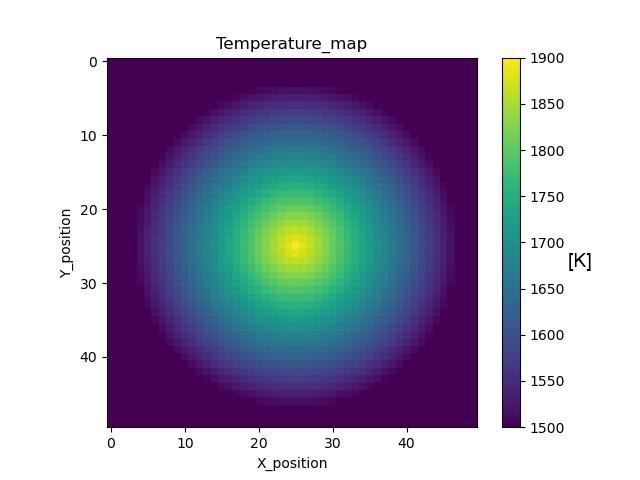
\includegraphics[width=0.8\textwidth]{figures/t_field.jpg}
    \caption{Temperature field used in validation}
    \label{fig: t_field}
\end{figure}


After obtaining a temperature field, the virtual experimental platform 
used the aforementioned 12 different emissivity models to generate 12 
different sets of experimental data. This approach simulated the radiative 
behavior of 12 hypothetical materials under identical temperature conditions 
in the virtual experiment platform.

{\linespread{1}
\begin{figure}[htbp]
    \centering
    \begin{minipage}{\textwidth}
        \centering
        \begin{subfigure}{0.45\textwidth}
            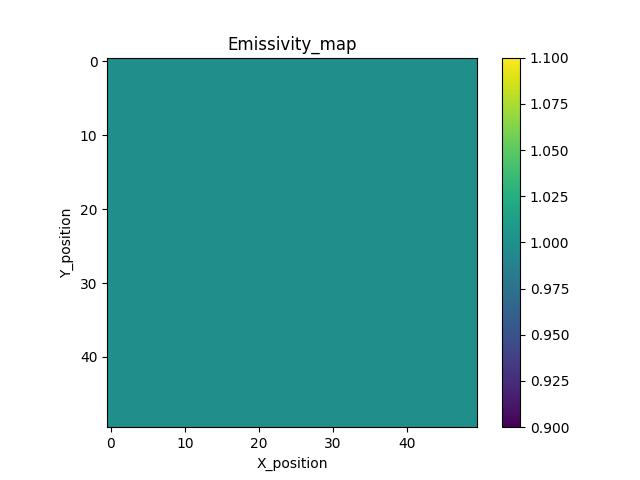
\includegraphics[width=\textwidth]{figures/raw_data/0/emi_field.jpg}
        \end{subfigure}
        \begin{subfigure}{0.45\textwidth}
            \centering
            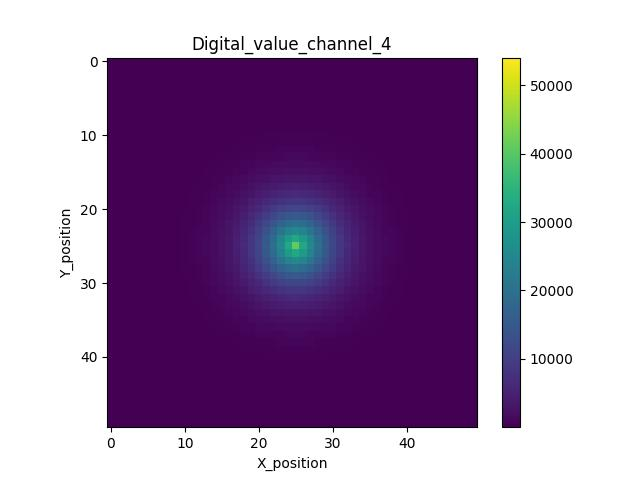
\includegraphics[width=\textwidth]{figures/raw_data/0/digital_value_channel_4.jpg}
        \end{subfigure}
        \subcaption{Black body}
        \label{fig: raw_data_0}
    \end{minipage}\\
    \begin{minipage}{\textwidth}
        \centering
        \begin{subfigure}{0.45\textwidth}
            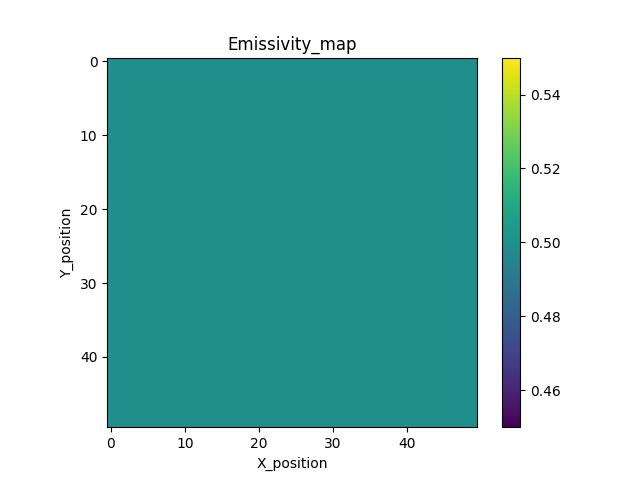
\includegraphics[width=\textwidth]{figures/raw_data/1/emi_field.jpg}
        \end{subfigure}
        \begin{subfigure}{0.45\textwidth}
            \centering
            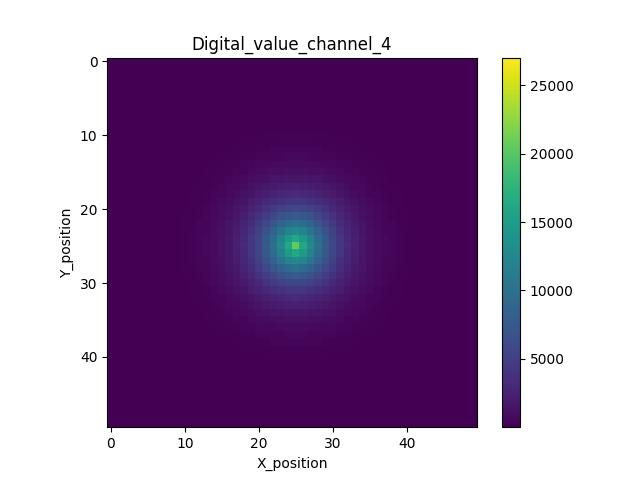
\includegraphics[width=\textwidth]{figures/raw_data/1/digital_value_channel_4.jpg}
        \end{subfigure}
        \subcaption{Gray body}
        \label{fig: raw_data_1}
    \end{minipage}\\
    \begin{minipage}{\textwidth}
        \centering
        \begin{subfigure}{0.45\textwidth}
            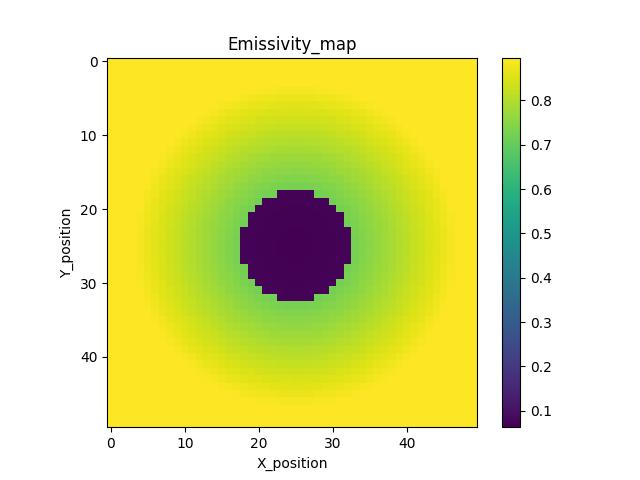
\includegraphics[width=\textwidth]{figures/raw_data/21/emi_field.jpg}
        \end{subfigure}
        \begin{subfigure}{0.45\textwidth}
            \centering
            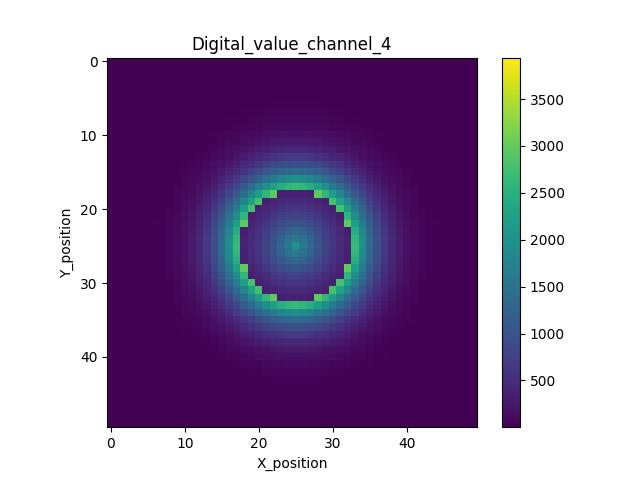
\includegraphics[width=\textwidth]{figures/raw_data/21/digital_value_channel_4.jpg}
        \end{subfigure}
        \subcaption{Model 1}
        \label{fig: raw_data_21}
    \end{minipage}\\
    \begin{minipage}{\textwidth}
        \centering
        \begin{subfigure}{0.45\textwidth}
            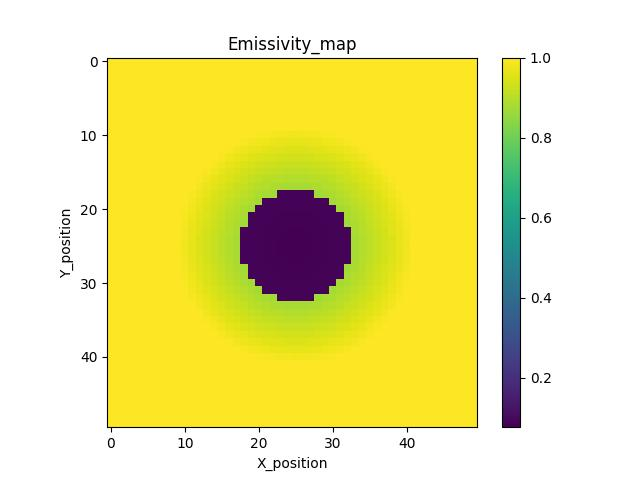
\includegraphics[width=\textwidth]{figures/raw_data/32/emi_field.jpg}
        \end{subfigure}
        \begin{subfigure}{0.45\textwidth}
            \centering
            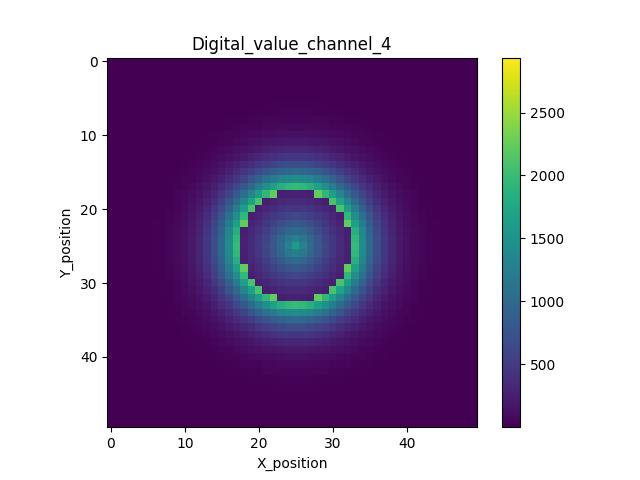
\includegraphics[width=\textwidth]{figures/raw_data/32/digital_value_channel_4.jpg}
        \end{subfigure}
        \subcaption{Model 8}
        \label{fig: raw_data_32}
    \end{minipage}
    \caption{Emissivity field and digital value of radiation intensity in channel 4 for 
    black body material(\subref{fig: raw_data_0}), gray body material(\subref{fig: raw_data_1}), 
    material based on model 1(\subref{fig: raw_data_21}) and model 8(\subref{fig: raw_data_32})}
    \label{fig: raw_data}
\end{figure}}

As a result, Fig.\ref{fig: raw_data} displays the emissivity fields generated by defferent
model along with their corresponding radiation intensities. To conserve space, 
digital values of channel 4 in each experiment data were chosen as 
representatives of the intensity data.


It can be observed that in blackbody and gray body materials, emissivity is not 
dependent on the material's temperature or status. As a result, the emissivity 
field exhibits a uniform color distribution. This characteristic also leads to a 
situation in the calculation of radiation intensity, where the physical values 
received by the virtual camera show a maximum at the center point and decrease 
as the temperature decreases.


However, in more general material models, such as Model 1 and Model 8, emissivity 
undergoes a discontinuity when the material transitions from the solid state to 
the liquid state. This is due to the fact that the emissivity of liquid phase 
is smaller than that of solid phase. Consequently, the radiation intensity 
received by the virtual camera decreases at the boundary when the material 
changes from solid to a liquid. Subsequently, at the center point, the radiation 
intensity emitted by the hypothetical material increases again due to the rise in 
temperature. This phenomenon results in a bright halo appearing in the digital 
value of channel 4 in the images. The center of this 
halo exhibits a point with higher brightness level.


Indeed, the non-uniform intensity distribution caused by different emissivity 
characteristics of materials can lead to challenges for the subsequent 
temperature estimation algorithm. The intensity distribution along wavelength 
differs due to the different emissivity model of the hypothetical material. 
Consequently, in the curve fit algorithm, the most suitable emissivity model for 
the current material may change accordingly. Therefore, particular attention 
should be given to the phase transition of the hypothetical material in the 
context of temperature estimation. 


After investigating the impact of different emissivity models on material 
radiative characteristics, it is necessary to explore the relationship between 
digital values of radiation intenstiy across different channels. 
Fig.\ref{fig: channel} displays the images of a material based on Model 1 at a 
temperature of 1900K, captured using 8 different channels. In this image, 
it can be observed that the intensity received by the virtual camera increases 
with the channel number.

\begin{figure}[htbp]
    \centering
    \begin{minipage}{0.10\textwidth}
        \centering
        \includegraphics[width=\textwidth]{figures/raw_data/21/color_bar.pdf}
    \end{minipage}
    \begin{minipage}{0.87\textwidth}
        \centering
        \begin{subfigure}{0.23\textwidth}
            \includegraphics[width=\textwidth]{figures/raw_data/21/channel_1.pdf}
            \caption{Channel 1}
        \end{subfigure}
        \begin{subfigure}{0.23\textwidth}
            \includegraphics[width=\textwidth]{figures/raw_data/21/channel_2.pdf}
            \caption{Channel 2}
        \end{subfigure}
        \begin{subfigure}{0.23\textwidth}
            \includegraphics[width=\textwidth]{figures/raw_data/21/channel_3.pdf}
            \caption{Channel 3}
        \end{subfigure}
        \begin{subfigure}{0.23\textwidth}
            \includegraphics[width=\textwidth]{figures/raw_data/21/channel_4.pdf}
            \caption{Channel 4}
        \end{subfigure}\\
        \begin{subfigure}{0.23\textwidth}
            \includegraphics[width=\textwidth]{figures/raw_data/21/channel_5.pdf}
            \caption{Channel 5}
        \end{subfigure}
        \begin{subfigure}{0.23\textwidth}
            \includegraphics[width=\textwidth]{figures/raw_data/21/channel_6.pdf}
            \caption{Channel 6}
        \end{subfigure}
        \begin{subfigure}{0.23\textwidth}
            \includegraphics[width=\textwidth]{figures/raw_data/21/channel_7.pdf}
            \caption{Channel 7}
        \end{subfigure}
        \begin{subfigure}{0.23\textwidth}
            \includegraphics[width=\textwidth]{figures/raw_data/21/channel_8.pdf}
            \caption{Channel 8}
        \end{subfigure}
    \end{minipage}
    \caption{Digital value of each channel by hypothetical material based on model 1
    and a linear temperature distribution with center temperature 1900K}
    \label{fig: channel}
\end{figure}


According to Wien's displacement law introduced in previous chapter, 
as described in Eq.\ref{eq: wiens_law}, when the hypothetical material's 
temperature is 1900K, it is easy to calculate the peak 
wavelength ($\lambda_{peak}$) as 1525nm. Consequently, it can be 
inferred that the spectral intensity of blackbody radiation emitted 
by the hypothetical material will increase with increasing wavelength 
across the entire observation range ($500-1000nm$). This characteristic 
aligns with the real experimental observation, where the spectral 
radiation intensity received by a camera increases with the channel 
number.

\subsection{Estimated temperature field and emissivity field}
After obtaining reliable experimental data, it is essential to perform 
temperature estimation algorithm to validate the accuracy of the 
temperature estimation algorithm. The temperature estimation algorithm 
will yield two primary results: the estimated temperature field and the 
simplified estimated emissivity field. These computational results 
will be presented:

\begin{enumerate}
    \item Estimated temperature field: The estimated temperature field represents 
    the spatial distribution of temperature across the observation area. This is 
    a most important output of the whole temperature estimation algorithm.

    \item Simplified estimated emissivity field: The simplified estimated 
    emissivity field denotes the variation of emissivity across the 
    observation area. It could be used to indentify the phase change area 
    and thus find the improvement potential.
\end{enumerate}


For visualization, the presentation of the computational results will be categorized based on the 
emissivity model used in the temperature estimation algorithm. As the 
experimental data for these temperature estimation algorithm use the 
same temperature distribution, relative error of temperature is employed here to 
represent the accuracy of the computations. To save space, the results 
of calculations for blackbody materials and materials based on Model 1 are selected for presentation.


In real experimental data, due to the limitations of the sensors, it is not 
possible to simultaneously observe the radiation intensity of the non-laser-heated 
region and the radiation intensity of the laser-heated region. In the 
virtual experimental platform, the temperature of the background region is 
assumed to be uniform, which is comparable to the real situations. 
Consequently, in order to avoid introducing statistical errors, the calculation 
results of the temperature estimation algorithm in background region can be 
considered as negligible.

\subsubsection{Linear model}

\begin{figure}[htbp]
    \centering
    \begin{minipage}{\textwidth}
        \centering
        \begin{subfigure}{0.325\textwidth}
            \centering
            \includegraphics[width=\textwidth]{figures/raw_data/21/linear/T_cal.jpg}
        \end{subfigure}
        \begin{subfigure}{0.325\textwidth}
            \centering
            \includegraphics[width=\textwidth]{figures/raw_data/21/linear/T_bias.jpg}
        \end{subfigure}
        \begin{subfigure}{0.325\textwidth}
            \centering
            \includegraphics[width=\textwidth]{figures/raw_data/21/linear/emi_cal.jpg}
        \end{subfigure}
        \subcaption{Material based on model 1}
    \end{minipage}\\
    \begin{minipage}{\textwidth}
        \centering
        \begin{subfigure}{0.325\textwidth}
            \centering
            \includegraphics[width=\textwidth]{figures/raw_data/5/linear/T_cal.jpg}
        \end{subfigure}
        \begin{subfigure}{0.325\textwidth}
            \centering
            \includegraphics[width=\textwidth]{figures/raw_data/5/linear/T_bias.jpg}
        \end{subfigure}
        \begin{subfigure}{0.325\textwidth}
            \centering
            \includegraphics[width=\textwidth]{figures/raw_data/5/linear/emi_cal.jpg}
        \end{subfigure}
        \subcaption{Material based on real iron data}
    \end{minipage}
    \caption{Calculation results of linear model}
    \label{fig: result_linear_model}
\end{figure}


Fig.\ref{fig: result_linear_model} demonstrate the calculation result on material based on 
model 1 and real data from iron. It can be found that the calculation result is more
stable in real data due to the material character. 


It can be observed that relative bias are present 
in the estimations based on two different materials. Moreover, this relative bias 
experiences a sudden change with increasing temperature, represented by a red 
circle in the figure. The reason behind this phenomenon can be considered as follows, 
at the boundary of the circle, the material undergoes a phase change from solid to liquid, 
leading to a rapid change in emissivity. The linear model is only able to  
simulate linear emissivity models, which fails to adequately fit the variations 
occurring at this point, resulting in significant deviations in the 
temperature estimations.


It can be found in table \ref{tab: statistic_results} that in the computation of linear models, 
calculation results based on real data exists relatively low average relative error and the lowest 
standard deviation. This indicates that the linear model maintains a higher 
level of consistency when performing calculations on real materials. It also 
achieves a maximum relative error of no more than 9.6\%. However, when 
performing calculations on other hypothetical materials, the linear model may 
produce relatively large errors, particularly for model 8, which has a high standard 
deviation, meaning the low consistency in the calculations. As mentioned 
in previous sections, this decrease in computational consistency could be attributed to the 
fact that the emissivity of materials based on model 8 undergoes a sudden change 
as the wavelength increases, which is a potential reason for the decline in 
calculation consistency.


\subsubsection{Linear square model}

\begin{figure}[htbp]
    \centering
    \begin{minipage}{\textwidth}
        \centering
        \begin{subfigure}{0.325\textwidth}
            \centering
            \includegraphics[width=\textwidth]{figures/raw_data/21/lin_square/T_cal.jpg}
        \end{subfigure}
        \begin{subfigure}{0.325\textwidth}
            \centering
            \includegraphics[width=\textwidth]{figures/raw_data/21/lin_square/T_bias.jpg}
        \end{subfigure}
        \begin{subfigure}{0.325\textwidth}
            \centering
            \includegraphics[width=\textwidth]{figures/raw_data/21/lin_square/emi_cal.jpg}
        \end{subfigure}
        \subcaption{Material based on model 1}
    \end{minipage}\\
    \begin{minipage}{\textwidth}
        \centering
        \begin{subfigure}{0.325\textwidth}
            \centering
            \includegraphics[width=\textwidth]{figures/raw_data/5/lin_square/T_cal.jpg}
        \end{subfigure}
        \begin{subfigure}{0.325\textwidth}
            \centering
            \includegraphics[width=\textwidth]{figures/raw_data/5/lin_square/T_bias.jpg}
        \end{subfigure}
        \begin{subfigure}{0.325\textwidth}
            \centering
            \includegraphics[width=\textwidth]{figures/raw_data/5/lin_square/emi_cal.jpg}
        \end{subfigure}
        \subcaption{Material based on real iron data}
    \end{minipage}
    \caption{Calculation results of linear square model}
    \label{fig: result_linear_square_model}
\end{figure}


Fig.\ref{fig: result_linear_square_model} presents the computational results of the 
linear square model for the virtual experimental data based on both model 1 and 
real iron. It can be observed that the results obtained by the linear square 
model do not exhibit the ring-like pattern that emerges with increasing temperature 
for the hypothetical material. This is because the linear square model possesses 
better capabilities to fit complex emissivity behaviors. In the emissivity plot 
on the right side, it is evident that the linear square model accurately 
reproduces the abrupt change in emissivity in the liquid region without 
causing a significant increase in temperature estimation errors. Thus, it can be 
concluded that the linear square model outperforms the linear model in terms 
of temperature estimation accuracy.


\subsubsection{Quadratic model}

\begin{figure}[htbp]
    \centering
    \begin{minipage}{\textwidth}
        \centering
        \begin{subfigure}{0.325\textwidth}
            \centering
            \includegraphics[width=\textwidth]{figures/raw_data/21/quad/T_cal.jpg}
        \end{subfigure}
        \begin{subfigure}{0.325\textwidth}
            \centering
            \includegraphics[width=\textwidth]{figures/raw_data/21/quad/T_bias.jpg}
        \end{subfigure}
        \begin{subfigure}{0.325\textwidth}
            \centering
            \includegraphics[width=\textwidth]{figures/raw_data/21/quad/emi_cal.jpg}
        \end{subfigure}
        \subcaption{Material based on model 1}
    \end{minipage}\\
    \begin{minipage}{\textwidth}
        \centering
        \begin{subfigure}{0.325\textwidth}
            \centering
            \includegraphics[width=\textwidth]{figures/raw_data/5/quad/T_cal.jpg}
        \end{subfigure}
        \begin{subfigure}{0.325\textwidth}
            \centering
            \includegraphics[width=\textwidth]{figures/raw_data/5/quad/T_bias.jpg}
        \end{subfigure}
        \begin{subfigure}{0.325\textwidth}
            \centering
            \includegraphics[width=\textwidth]{figures/raw_data/5/quad/emi_cal.jpg}
        \end{subfigure}
        \subcaption{Material based on real iron data}
    \end{minipage}
    \caption{Calculation results of quadratic model}
    \label{fig: result_quadratic_model}
\end{figure}


Unlike the previously mentioned linear square model, the quadratic model has one 
fewer parameter, resulting in fewer degrees of freedom for the emissivity model. 
In fact, based on Eq.\ref{eq: emi_quad} from the paper, this mathematical 
model ss y-axis symmetry. Considering the physical meaning of emissivity, 
it can only be used to fit emissivity models that are either monotonically 
increasing or monotonically decreasing.

As a result, as shown in Fig.\ref{fig: result_quadratic_model}, it can be observed 
that in the computations based on model 1 for the material, the performance 
of the temperature estimation algorithm is better at the central point 
(the location with the highest temperature) compared to other regions due to less 
variations in emissivity.
The results of the emissivity field demonstrate that the algorithm accurately 
identifies the boundary regions between liquid and solid materials.

However, for computations involving real materials, the algorithm struggles to 
accurately estimate the emissivity of hypothetical materials, leading to errors in 
temperature calculations. Nevertheless, it is still evident that the 
temperature estimation algorithm based on the quadratic model performs better 
on real materials compared to hypothetical materials.

\subsubsection{Exponential model}

\begin{figure}[htbp]
    \centering
    \begin{minipage}{\textwidth}
        \centering
        \begin{subfigure}{0.325\textwidth}
            \centering
            \includegraphics[width=\textwidth]{figures/raw_data/21/exp/T_cal.jpg}
        \end{subfigure}
        \begin{subfigure}{0.325\textwidth}
            \centering
            \includegraphics[width=\textwidth]{figures/raw_data/21/exp/T_bias.jpg}
        \end{subfigure}
        \begin{subfigure}{0.325\textwidth}
            \centering
            \includegraphics[width=\textwidth]{figures/raw_data/21/exp/emi_cal.jpg}
        \end{subfigure}
        \subcaption{Material based on model 1}
    \end{minipage}\\
    \begin{minipage}{\textwidth}
        \centering
        \begin{subfigure}{0.325\textwidth}
            \centering
            \includegraphics[width=\textwidth]{figures/raw_data/5/exp/T_cal.jpg}
        \end{subfigure}
        \begin{subfigure}{0.325\textwidth}
            \centering
            \includegraphics[width=\textwidth]{figures/raw_data/5/exp/T_bias.jpg}
        \end{subfigure}
        \begin{subfigure}{0.325\textwidth}
            \centering
            \includegraphics[width=\textwidth]{figures/raw_data/5/exp/emi_cal.jpg}
        \end{subfigure}
        \subcaption{Material based on real iron data}
    \end{minipage}
    \caption{Calculation results of exponential model}
    \label{fig: result_exponential_model}
\end{figure}


In the exponential model, the emissivity model follows the form of an 
exponential function. The two parameters in the emissivity model allow for 
translation and deformation of the exponential function. This enables the 
temperature estimation algorithm to be applicable to a wider range of materials 
with different emissivity characteristics. Fig.\ref{fig: result_exponential_model} 
presents the results of this temperature estimation algorithm for materials 
based on \mbox{model 1} and real iron.


Due to the physical meaning of emissivity, the value of emissivity is defined 
within the range of 0 to 1. Thus, constraints must be imposed on the 
emissivity model. Thus, calculated from Eq.\ref{eq: emi_exp}, the following 
constraints can be introduced:


\begin{equation}
    -a \cdot \lambda_{norm} - b \leq 0
\end{equation}


Therefore, the derivative of emissivity with respect to wavelength is obtained as:


\begin{equation}
    \frac{d\varepsilon(\lambda)}{d\lambda_{norm}} = -a \cdot e^{-a \cdot \lambda_{norm} - b}
\end{equation}

For each data point, the emissivity computed based on the exponential model 
is either monotonically increasing or decreasing, depending on the sign of 
parameter $a$. This characteristic of the model leads to an increase in 
computational speed and a decrease in 
computational accuracy when strong non-monotonic behavior is observed in 
the emissivity characteristics of the material.

In Fig.\ref{fig: result_exponential_model}, it is evident that material based on 
\mbox{model 1} exhibits an almost linear relationship between emissivity and 
wavelength in the liquid state. This enables the temperature estimation 
algorithm to accurately calculate the boundary region between the liquid and 
solid states and achieve high computational precision within the liquid 
state region.

However, when applying the temperature estimation algorithm to real iron data, 
it fails to accurately calculate the emissivity values. This discrepancy is due 
to the fluctuation observed in the emissivity of real iron as a function of 
wavelength. The emissivity of iron in the liquid state is closer to the 
numerically derived values of the algorithm than in the solid state, leading 
to erroneous conclusions of higher computational accuracy at the central points.


\subsubsection{Mixed model}
Eq.\ref{eq: emi_mix_gen} indicates that the mixed model is composed of two 
components: a low-temperature emissivity model and a high-temperature emissivity 
model. This approach offers a significant advantage as the temperature 
estimation algorithm can fit to the different emissivity 
characteristics observed in the liquid and solid regions. But the computational 
time has significantly increased due to the utilization of two different 
emissivity models.


\begin{equation}
    \label{eq: emi_mix}
    \varepsilon(\lambda) = \begin{cases} 
      a \cdot \lambda_{norm}^2 + b \cdot \lambda_{norm} + c &   T \leq T_{melt} \\
      \exp(-a \cdot \lambda_{norm} - b) & T > T_{melt}
    \end{cases}
  \end{equation}


In this work, the low-temperature emissivity model is represented by linear 
square model, while the high-temperature emissivity model is described using 
exponential model. This choice is driven by the fact that the emissivity of the 
hypothetical material exhibits significant fluctuations in the solid-state 
region, making it more suitable to be computed using linear 
square model to better capture its behavior. Conversely, in the liquid state 
region, the emissivity of the hypothetical material exhibits relatively smaller 
fluctuations, making it possible to use a faster computational 
exponential model without decreasing the accuracy.


\begin{figure}[htbp]
    \centering
    \begin{minipage}{\textwidth}
        \centering
        \begin{subfigure}{0.325\textwidth}
            \centering
            \includegraphics[width=\textwidth]{figures/raw_data/0/mix/T_cal.jpg}
        \end{subfigure}
        \begin{subfigure}{0.325\textwidth}
            \centering
            \includegraphics[width=\textwidth]{figures/raw_data/0/mix/T_bias.jpg}
        \end{subfigure}
        \begin{subfigure}{0.325\textwidth}
            \centering
            \includegraphics[width=\textwidth]{figures/raw_data/0/mix/emi_cal.jpg}
        \end{subfigure}
        \subcaption{Black body material}
    \end{minipage}\\
    \begin{minipage}{\textwidth}
        \centering
        \begin{subfigure}{0.325\textwidth}
            \centering
            \includegraphics[width=\textwidth]{figures/raw_data/21/mix/T_cal.jpg}
        \end{subfigure}
        \begin{subfigure}{0.325\textwidth}
            \centering
            \includegraphics[width=\textwidth]{figures/raw_data/21/mix/T_bias.jpg}
        \end{subfigure}
        \begin{subfigure}{0.325\textwidth}
            \centering
            \includegraphics[width=\textwidth]{figures/raw_data/21/mix/emi_cal.jpg}
        \end{subfigure}
        \subcaption{Material based on model 1}
    \end{minipage}\\
    \begin{minipage}{\textwidth}
        \centering
        \begin{subfigure}{0.325\textwidth}
            \centering
            \includegraphics[width=\textwidth]{figures/raw_data/5/mix/T_cal.jpg}
        \end{subfigure}
        \begin{subfigure}{0.325\textwidth}
            \centering
            \includegraphics[width=\textwidth]{figures/raw_data/5/mix/T_bias.jpg}
        \end{subfigure}
        \begin{subfigure}{0.325\textwidth}
            \centering
            \includegraphics[width=\textwidth]{figures/raw_data/5/mix/emi_cal.jpg}
        \end{subfigure}
        \subcaption{Material based on real iron data}
    \end{minipage}
    \caption{Calculation results of mixed model}
    \label{fig: result_mixed_model}
\end{figure}


From Fig.\ref{fig: result_mixed_model}, it is evident that the mixed model 
accurately identifies the boundaries between the liquid and solid regions 
for both model 1 based material and real iron-based material. 
Additionally, it accurately recognizes the regions that require 
recalculations in the case of blackbody materials. This indicates that 
the model is applicable to materials with different emissivity characteristics.


Regarding the temperature estimation results, the model demonstrates high 
precision in calculating temperatures for blackbody materials and materials 
based on model 1. In these cases, the error in the center region is less than 7\%. 
However, the model shows a region of relatively lower accuracy when 
applied to real iron-based material. In this region, the emissivity values 
are erroneously computed as 1, leading to an increase in temperature 
calculation bias. This discrepancy can be attributed to the use of the 
exponential model in the temperature estimation algorithm, as mentioned 
earlier, which introduces errors when calculating the emissivity 
of real iron in its liquid state.


\section{Statistical results and analysis}

After obtaining all calculation results, some statistical results can be found in 
tabel \ref{tab: statistic_results}. To mitigate any negative impact of background 
regions on the statistical results of the temperature estimation algorithm, 
only the computation results from the central area of the observation 
area are considered here. As linear temperature distribution 
is employed for the hypothetical materials, temperature is used to determine 
whether the point is within 
the central area. These conditions can be formulated as follows:


\begin{equation}
    P = \begin{cases}
        P_{center}  & T \geq T_{edge} \\
        P_{background}  & T < T_{edge}
    \end{cases}
    \label{eq: T_edge}
\end{equation}


With $T_{edge} = 1200K$ for materials based on model and $T_{edge} = 1600K$ for materials based 
on real iron data. This is due to the fact that in the virtual experimental 
platform, the temperature of the background area in the experiments based on 
real iron data is set to $1500K$.


Table \ref{tab: statistic_results} presents the statistical results of five 
different temperature estimation algorithms: linear model, linear square model, 
quadratic model, exponential model and mixed model. These algorithms were 
applied to blackbody materials, real materials, and materials based on \mbox{Model 1-9}. 
The statistical metrics calculated for each algorithm include:


\begin{enumerate}
    \item Mean Difference(Difference)
    \item Mean Relative Error(Rel. difference)
    \item Standard Deviation(SD)
    \item Maximum Relative Error
    \item Minimum Relative Error
\end{enumerate}

\subsubsection{Mean Difference}
The mean difference describes the difference between the calculated 
temperature $T_{cal}$ and the actual temperature $T_{act}$. It intuitively 
demonstrates the accuracy of the temperature estimation algorithm. It is 
defined by the following equation:

\begin{equation}
    {E} = \overline{T_{cal} - T_{act}} 
\end{equation}

\subsubsection{Mean Relative Error}
The mean relative error describes the relative difference between the calculated 
temperature $T_{cal}$ and the actual temperature $T_{act}$. To avoid mutual 
cancellation between positive and negative deviations, the absolute value of 
the relative deviation is used here. The mathematical equation can be found as follows:

\begin{equation}
    {E}_{rel} = \overline{\left\lvert \frac{T_{cal} - T_{act}}{T_{act}}\right\rvert }
\end{equation}

\subsubsection{Standard Deviation}
The standard deviation is used to describe the distribution of differences 
between the calculated temperature $T_{cal}$ and the actual 
temperature $T_{act}$. Since a linear temperature distribution is used, the 
temperature range of materials within the observed area is relatively large. 
Hence, this standard deviation can be used to characterize the consistency of the 
temperature estimation algorithm's results under different temperature conditions.
The definition can be found by the following equation:

\begin{equation}
    \sigma = \sqrt{\frac{\sum {\left\lvert T_{cal} - T_{act}\right\rvert }^2}{N}} 
\end{equation}

With $N$ represents the number of points involved in the statistical analysis.

\subsubsection{Min. and Max. Relative Error}
These two parameters describe the maximum and minimum values of the relative 
difference between the calculated temperature $T_{cal}$ and the actual temperature 
$T_{act}$ over the entire statistical region. These parameters can be used to 
observe the maximum and minimum errors caused by the temperature estimation 
algorithm. This allows for a visual assessment of the effectiveness boundaries 
of the temperature estimation algorithm's results.


{\linespread{1}
\begin{sidewaystable}[htbp]
    \centering
    \caption{Calculation results from different models}
    \label{tab: statistic_results}
    \begin{tabular}{lccccccccccc}
        \hline
        & \multicolumn{1}{c}{Black body} & \multicolumn{1}{c}{Iron} & Model 1 & Model 2 & Model 3 & Model 4 & Model 5 & Model 6 & Model 7 & Model 8 & Model 9 \\ \hline
        \multicolumn{12}{c}{Linear}                                                                                                                                                         \\ \hline
        Difference {[}K{]}      & 20.7                           & -151.7                        & 129.5   & 38.8    & 58.6    & 116.5   & -4.8    & -39.6   & -161.6  & 445.5   & 27.2     \\
        Rel. difference         & 0.02                           & 0.08                          & 0.08    & 0.03    & 0.04    & 0.08    & 0.02    & 0.04    & 0.11    & 0.32    & 0.02     \\
        SD {[}K{]}              & 7.06                           & 9.56                          & 115.31  & 44.97   & 73.78   & 98.33   & 57.27   & 104.74  & 112.38  & 157.94  & 20.80    \\
        Max. difference {[}K{]} & 0.029                          & 0.096                         & 0.160   & 0.073   & 0.145   & 0.140   & 0.167   & 0.170   & 0.263   & 0.489   & 0.057    \\
        Min. difference {[}K{]} & 0.006                          & 0.076                         & 0.0001  & 0.0004  & 0.0001  & 0.0001  & 0.00    & 0.0001  & 0.001   & 0.031   & 0.0003   \\ \hline
        \multicolumn{12}{c}{Linear square}                                                                                                                                                   \\ \hline
        Difference {[}K{]}      & 38.7                           & 30.8                          & 102.9   & -13.1   & 24.4    & 72.9    & -31.1   & 96.5    & -122.5  & 423.9   & -10.6   \\
        Rel. difference         & 0.03                           & 0.02                          & 0.07    & 0.03    & 0.03    & 0.05    & 0.02    & 0.07    & 0.08    & 0.30    & 0.03    \\
        SD {[}K{]}              & 23.95                          & 6.88                          & 8.21    & 42.45   & 36.18   & 11.12   & 57.39   & 27.09   & 45.99   & 93.41   & 58.86   \\
        Max. difference {[}K{]} & 0.074                          & 0.079                         & 0.105   & 0.059   & 0.071   & 0.088   & 0.101   & 0.115   & 0.118   & 0.379   & 0.093   \\
        Min. difference {[}K{]} & 0.006                          & 0.013                         & 0.03    & 0.000   & 0.0001  & 0.031   & 0.0001  & 0.011   & 0.018   & 0.03    & 0.0001  \\ \hline
        \multicolumn{12}{c}{Quadratic}                                                                                                                                                 \\ \hline
        Difference {[}K{]}      & 19.3                           & -151.7                        & 104.7   & 41.5    & 8.6     & 88.1    & 76.7    & -47.8   & -212.7  & 509.9   & 113.1   \\
        Rel. difference         & 0.01                           & 0.09                          & 0.09    & 0.09    & 0.04    & 0.10    & 0.11    & 0.03    & 0.14    & 0.37    & 0.12    \\
        SD {[}K{]}              & 4.07                           & 9.56                          & 194.96  & 214.93  & 144.50  & 216.52  & 239.63  & 96.18   & 117.62  & 167.72  & 234.07  \\
        Max. difference {[}K{]} & 0.022                          & 0.096                         & 0.336   & 0.329   & 0.280   & 0.352   & 0.321   & 0.166   & 0.280   & 0.630   & 0.341   \\
        Min. difference {[}K{]} & 0.006                          & 0.076                         & 0.005   & 0.003   & 0.000   & 0.005   & 0.0003  & 0.0001  & 0.092   & 0.031   & 0.003   \\ \hline
        \multicolumn{12}{c}{Exponential}                                                                                                                                                   \\ \hline
        Difference {[}K{]}      & 20.5                           & -147.3                        & 102.9   & -12.9   & 24.4    & 72.9    & -60.5   & 96.6    & -406.4  & 318.2   & -91.6   \\
        Rel. difference         & 0.01                           & 0.08                          & 0.07    & 0.03    & 0.03    & 0.05    & 0.04    & 0.07    & 0.45    & 0.325   & 0.235    \\
        SD {[}K{]}              & 16.70                          & 24.63                         & 8.23    & 42.15   & 36.19   & 11.14   & 56.69   & 27.04   & 523.51  & 385.45  & 343.71  \\
        Max. difference {[}K{]} & 0.075                          & 0.096                         & 0.105   & 0.056   & 0.071   & 0.088   & 0.101   & 0.115   & 0.644   & 0.630   & 0.452   \\
        Min. difference {[}K{]} & 0.006                          & 0.013                         & 0.031   & 0.00    & 0.0001  & 0.03    & 0.0005  & 0.012   & 0.031   & 0.002   & 0.003   \\ \hline
        \multicolumn{12}{c}{Mixed model}                                                                                                                                                   \\ \hline
        Difference {[}K{]}      & 14.6                           & -34.6                         & 102.9   & -12.9   & 24.4    & 72.9    & -31.1   & 96.6    & -122.5  & 424.16  & -10.6    \\
        Rel. difference         & 0.01                           & 0.02                          & 0.07    & 0.03    & 0.03    & 0.05    & 0.02    & 0.07    & 0.08    & 0.30    & 0.025    \\
        SD {[}K{]}              & 6.17                           & 53.49                         & 8.22    & 42.14   & 36.19   & 11.13   & 57.39   & 27.04   & 45.98   & 93.88   & 85.86  \\
        Max. difference {[}K{]} & 0.017                          & 0.096                         & 0.105   & 0.056   & 0.071   & 0.088   & 0.101   & 0.115   & 0.118   & 0.382   & 0.093   \\
        Min. difference {[}K{]} & 0.00                           & 0.006                         & 0.03    & 0.000   & 0.0001  & 0.031   & 0.000   & 0.012   & 0.018   & 0.031   & 0.0001  
    \end{tabular}
\end{sidewaystable}
}

\subsection{Performance of different temperature estimation algorithms}
After obtaining the statistical results of the temperature estimation algorithm, 
it is necessary to analyze these results. Since the statistical outcomes 
encompass the calculations of various temperature estimation algorithms 
for different materials, the analysis consists of two main parts: one involves 
the performance analysis of different temperature estimation algorithms, 
while the other concerns the performance analysis of the temperature estimation 
algorithm for different materials.


In Table \ref{tab: statistic_results}, it can be observed that each temperature 
estimation algorithm produces different results for the same material. 


When applied to blackbody materials, all algorithms achieve accuracy
within 5\% error. However, it is evident that the linear square model 
exhibits lower precision compared to other models, and simultaneously, 
the standard deviation of its calculations is significantly higher than 
that of other temperature estimation algorithms. This discrepancy could be 
attributed to the linear square model having an additional parameter, which 
makes the curve-fitting process more prone to encountering local minima and 
prematurely terminating the computation.


Indeed, in addition to linear square model's performance on blackbody materials, the temperature 
estimation algorithm based on the linear square model consistently achieves 
lower relative errors and standard deviations compared to other temperature 
estimation algorithms when applied to different materials. This indicates that 
the linear square model not only attains higher accuracy but also exhibits a 
higher level of computation consistency.


In contrast to the linear square model, the temperature estimation algorithm 
based on the quadratic model exhibits lower consistency in computing results 
for hypothetical materials in this work. The standard deviation for this 
metric is close to or exceeds 100K. This indicates that the temperature 
estimation algorithm based on the quadratic model cannot demonstrate 
high consistency in the calculations of the virtual materials used in this 
work. This is attributed to the emissivity characteristics of the hypothetical materials 
used in this study, which do not conform well to the profile of the quadratic 
function. Consequently, the curve fit algorithm fails to find stable global 
optimal points, resulting in lower consistency in the computed results.


The temperature estimation algorithm based on the exponential model demonstrates 
comparable accuracy and consistency to the temperature estimation algorithm 
based on the linear square model when applied to blackbody material
and materials based on model 1, 2, 3, 4, and 6. Furthermore, it offers 
significant time savings in computational efforts. In situations where the 
emissivity variation is limited, this model exhibits a higher propensity to 
yield stable local optima, making it particularly suitable for application 
in the liquid phase region of hypothetical materials based on models.


It is evident from the results that different temperature estimation algorithms 
exhibit varying performance when applied to experimental data from different 
materials. To address this, the author proposes utilizing a temperature estimation 
algorithm based on the mixed model to effectively combine the advantages of 
different estimation approaches, especially for materials with complex emissivity 
characteristics. Table \ref{tab: statistic_results} illustrates that the mixed 
model outperforms the linear square model and exponential model in the 
computation of blackbody materials, showing better accuracy and consistency. 
Moreover, across all other models, the temperature estimation algorithm based 
on the mixed model consistently yields the better result in the two 
original temperature estimation algorithms.

\subsection{Performance of temperature estimation algorithm between different materials}

\begin{figure}[htbp]
    \centering
    \begin{subfigure}{\textwidth}
        \includegraphics[width=\textwidth]{figures/diff_rel.jpg}
        \subcaption{Mean relative error}
    \end{subfigure}\\
    \begin{subfigure}{\textwidth}
        \includegraphics[width=\textwidth]{figures/diff_std.jpg}
        \subcaption{Standard deviation}
    \end{subfigure}
    \caption{Mean relative error and standard deviation of calculation results}
    \label{fig: result_final_analysis}
\end{figure}

Fig.\ref{fig: result_final_analysis} presents the computational results of 
temperature estimation using five different temperature estimation algorithms 
on various hypothetical materials. 


In temperature estimation for blackbody materials, all emissivity models yield accurate 
results with acceptable consistency. This phenomenon arises from the fact that 
the emissivity of blackbody materials remains constant regardless of wavelength.
This characteristic allows the avoidance of emissivity's impact on the estimated 
temperature during the curve fitting process, thus enhancing both the accuracy 
and consistency of the calculations.


In the calculation of hypothetical material based on real iron data, 
the temperature estimation algorithms based on the linear square model and the 
mixed model exhibit mean relative errors below 5\%. Other models also achieve 
mean relative errors below 10\%. Concerning computational consistency, 
apart from the mixed model and exponential model, the standard deviations of the 
remaining models are within 10K, while the mixed model and exponential model have 
standard deviations exceeding 20K. This phenomenon is attributed to the exponential 
model's inability to adequately 
fit the emissivity behavior within the liquid phase region of real iron data. 
Consequently, this inadequacy leads to a decrease in the accuracy of temperature 
estimation. Meanwhile, it is noteworthy that the temperature estimation algorithm 
based on the mixed model alters the emissivity model during its operation, thereby 
resulting in a reduction in the consistency of the computed results.


In contrast to the first two materials, for materials based on model 1, 2, 3, 4, 5, 
6, and 9, the mixed model and linear square model exhibit similar performance 
in temperature estimations. Both models are capable of achieving a mean relative 
error in temperature estimation of less than 10\%. On the other hand, the quadratic 
model demonstrates relatively inferior performance. Its computational result 
exhibit both higher mean relative error and lower consistency in calculations. 
This observation suggests that the temperature estimation algorithm based on the 
quadratic model is not suitable for calculating temperatures of the hypothetical 
materials mentioned in this work. Conversely, the temperature estimation algorithms 
based on the linear square model and the mixed model can achieve higher precision 
in temperature estimation for these hypothetical materials.


For models 7 and 8, all temperature estimation algorithms exhibit lower 
computational accuracy and consistency. Particularly in model 8, 
none of the five temperature estimation algorithms are capable of providing 
effective temperature estimation results. This issue arises from the inability 
of these algorithms to fit the emissivity behavior of model 8, leading to 
ineffective temperature estimation results. Consequently, it is evident that the 
emissivity model plays a crucial role in temperature estimation algorithms, 
serving as a key determinant of their accuracy and consistency.


\section{System limitations and boundaries}
In the aforementioned analysis, it can be observed that the virtual 
experimentation platform, along with the temperature estimation system, 
are not devoid of imperfections. During utilization, they also exhibit 
certain limitations and systemic boundaries.


\subsection{Range of material data in virtual experiment platform}
As mentioned earlier, the emissivity of the hypothetical materials used in the virtual experiment 
platform is primarily determined by two terms. The first term is wavelength related, while the 
second term temperature related. 
$$0\varepsilon(\lambda, T) = \varepsilon _{raw}(\lambda) \cdot K_T(T)$$
It follows that when the virtual experiment platform generates 
experimental data, the physical meaning of the parameters of the experiment setup (such as temperature of the hypothetical material 
and the wavelength range of the virtual multispectralmeter) needs to be ensured. 
Although the extrapolation method was employed in the work to extend the range of emissivity data and prevent 
computational errors, this practice still contributes to a reduction in the reality 
of the generated experimental data.

\begin{figure}[htbp]
    \centering
    \begin{subfigure}{0.49\textwidth}
        \centering
        \includegraphics[width=\textwidth]{figures/emissivity_31_1.jpg}
        \caption{}
    \end{subfigure}
    \begin{subfigure}{0.49\textwidth}
        \centering
        \includegraphics[width=\textwidth]{figures/extrapolation_demo.jpg}
        \caption{}
    \end{subfigure}
    \caption{Original emissivity data and extrapolated emissivity data based on model 7 \cite{Taunay.2020b}}
    \label{fig: extrapolation_demo}
\end{figure}


Fig.\ref{fig: extrapolation_demo} illustrates a comparison between the extrapolated emissivity 
data and the original emissivity data. It is evident from the graph that beyond the wavelength 
range covered by the original data, the computer extends the domain of the original data using a 
linear extrapolation approach. The approach is based on the gradient of the original data at its 
boundaries for computation. This approach introduces uncertainty into the physical meaning. In this 
work, the emissivity of the hypothetical material should between 0 and 1, which should be
defined in the extrapolation process.


\subsection{Performance of temperature estimation algorithm at high target temperature}
As previously mentioned, a material's emitted blackbody radiation exhibits a peak that shifts towards 
shorter wavelengths as the temperature increases, accompanied by an increase in intensity. This 
phenomenon introduces alterations in the observed intensity patterns received by the virtual 
multispectral meter employed in this study. Earlier in the work, the accuracy of the temperature 
estimation algorithm was assessed within the temperature range of 1000-1900K. In these applications, 
the radiation peaks fell outside the range of wavelengths detected by the multispectral meter, 
meaning that across all experimental data, the digital values increased with an increase in the 
channel number.


However, as the temperature reaches 3500K, the radiation peak can be computed to be at 808nm, which 
falls within the wavelength range detectable by the virtual multispectral meter. Consequently, 
there emerges the possibility of the digital value of channel 7 being lower than that of 
channel 6 as presented in Fig.\ref{fig: channel_3500}. This occurrence may potentially introduce additional complexities to the 
temperature estimation algorithm, necessitating the validation of the algorithm's consistency 
under high-temperature conditions.


Hence, in order to verify the temperature estimation algorithm's computational capabilities for 
high-temperature materials, the virtual experimental platform conducted observations at 3500K for 
blackbody materials, iron, and hypothetical materials based on models 1, 2, 8, and 9. 
Due to the range limitation issue of the original data mentioned earlier, certain modifications 
were applied to the emissivity models of all hypothetical materials.


For the blackbody material, the emissivity remained unchanged. The emissivity model for iron was 
extended using extrapolation approach. As for the other hypothetical materials, the emissivity 
values were unchanged compared with previous experiments by altering the reference 
temperature $T_{ref}$ in the temperature factor. Since the hypothetical material is at liquid phase 
in the observation area, the phase change effect in emissivity model is then removed. The experiment data 
can be found in Fig.\ref{fig: data_3500}. It is evident that the emissivity of the hypothetical 
materials decreases with an increase in temperature. However, in contrast to 
previous findings, no phase transitions occurred within the observed range of 2500-3500K.
Consequently, there are no abrupt changes or discontinuities observed in the emissivity 
field within this temperature range.

\begin{figure}[htbp]
    \centering
    \begin{subfigure}{0.49\textwidth}
        \centering
        \includegraphics[width=\textwidth]{figures/t_field_3500linear.jpg}
        \subcaption{Temperature field}
    \end{subfigure}
    \begin{subfigure}{0.49\textwidth}
        \centering
        \includegraphics[width=\textwidth]{figures/raw_data/21/T3500/emi_field.jpg}
        \subcaption{Emissivity of material based on model 1}
    \end{subfigure}
    \caption{Temperature field and emissivity field of material based on model 1 at 3500K}
    \label{fig: data_3500}
\end{figure}

\begin{figure}[htbp]
    \centering
    \begin{minipage}{0.10\textwidth}
        \centering
        \includegraphics[width=\textwidth]{figures/raw_data/21/T3500/color_bar.pdf}
    \end{minipage}
    \begin{minipage}{0.87\textwidth}
        \centering
        \begin{subfigure}{0.23\textwidth}
            \includegraphics[width=\textwidth]{figures/raw_data/21/T3500/channel_1.pdf}
            \caption{Channel 1}
        \end{subfigure}
        \begin{subfigure}{0.23\textwidth}
            \includegraphics[width=\textwidth]{figures/raw_data/21/T3500/channel_2.pdf}
            \caption{Channel 2}
        \end{subfigure}
        \begin{subfigure}{0.23\textwidth}
            \includegraphics[width=\textwidth]{figures/raw_data/21/T3500/channel_3.pdf}
            \caption{Channel 3}
        \end{subfigure}
        \begin{subfigure}{0.23\textwidth}
            \includegraphics[width=\textwidth]{figures/raw_data/21/T3500/channel_4.pdf}
            \caption{Channel 4}
        \end{subfigure}\\
        \begin{subfigure}{0.23\textwidth}
            \includegraphics[width=\textwidth]{figures/raw_data/21/T3500/channel_5.pdf}
            \caption{Channel 5}
        \end{subfigure}
        \begin{subfigure}{0.23\textwidth}
            \includegraphics[width=\textwidth]{figures/raw_data/21/T3500/channel_6.pdf}
            \caption{Channel 6}
        \end{subfigure}
        \begin{subfigure}{0.23\textwidth}
            \includegraphics[width=\textwidth]{figures/raw_data/21/T3500/channel_7.pdf}
            \caption{Channel 7}
        \end{subfigure}
        \begin{subfigure}{0.23\textwidth}
            \includegraphics[width=\textwidth]{figures/raw_data/21/T3500/channel_8.pdf}
            \caption{Channel 8}
        \end{subfigure}
    \end{minipage}
    \caption{Digital value of each channel by hypothetical material based on model 1
    and a linear temperature distribution with center temperature 3500K}
    \label{fig: channel_3500}
\end{figure}

\subsection{Emissivity model in temperature estimation algorithm}
As analyzed in the preceding sections, the emissivity model plays a decisive role in 
determining the accuracy of the temperature estimation algorithm. It significantly 
influences the precision and consistency of the results obtained. However, the quadratic 
model exhibited unsatisfactory performance on the hypothetical materials utilized in this study, 
thus, it will not be employed for temperature estimation on high-temperature materials. 
Additionally, since phase transitions are absent in the virtual experiments conducted here 
with the hypothetical materials, the use of a mixed model is deemed unnecessary.




Therefore, the evaluation of temperature estimation algorithm's performance 
on the hypothetical material at high temperatures involves testing of the linear model, 
linear square model and exponential model.


\subsubsection{Linear model}
It is apparent that the linear model cannot provide accurate temperature estimations 
for the hypothetical materials at high temperatures. This limitation stems from the 
relatively low degrees of freedom inherent to the linear model. The precision of the 
temperature estimation algorithm at 3500K is lower than that at 1900K. The details 
can be found in table\ref{tab: statistic_results_3500}.
Nevertheless, 
the program is still capable of reliably calculating the trend of temperature variations. 
This observation underscores that the radiation peak can be fitted by the 
program.


\begin{figure}[htbp]
    \centering
    \begin{minipage}{\textwidth}
        \centering
        \begin{subfigure}{0.325\textwidth}
            \centering
            \includegraphics[width=\textwidth]{figures/raw_data/21/T3500/linear/T_cal.jpg}
        \end{subfigure}
        \begin{subfigure}{0.325\textwidth}
            \centering
            \includegraphics[width=\textwidth]{figures/raw_data/21/T3500/linear/T_bias.jpg}
        \end{subfigure}
        \begin{subfigure}{0.325\textwidth}
            \centering
            \includegraphics[width=\textwidth]{figures/raw_data/21/T3500/linear/emi_cal.jpg}
        \end{subfigure}
        \subcaption{Material based on model 1}
    \end{minipage}\\
    \begin{minipage}{\textwidth}
        \centering
        \begin{subfigure}{0.325\textwidth}
            \centering
            \includegraphics[width=\textwidth]{figures/raw_data/5/T3500/linear/T_cal.jpg}
        \end{subfigure}
        \begin{subfigure}{0.325\textwidth}
            \centering
            \includegraphics[width=\textwidth]{figures/raw_data/5/T3500/linear/T_bias.jpg}
        \end{subfigure}
        \begin{subfigure}{0.325\textwidth}
            \centering
            \includegraphics[width=\textwidth]{figures/raw_data/5/T3500/linear/emi_cal.jpg}
        \end{subfigure}
        \subcaption{Material based on real iron data}
    \end{minipage}
    \caption{Calculation results of linear model at 3500K}
    \label{fig: result_linear_model_3500}
\end{figure}


\subsubsection{Linear square model}
It can be observed that the linear square model achieves relative errors 
within 10\% for temperature estimation on both iron-based materials and materials based on \mbox{model 1}. 
This model accurately computes the temperatures of various hypothetical materials. 
However, it still has limitations. Specifically, estimation of emissivity at high temperatures still has 
potential to be improved. 
This issue arises due to the complexity introduced 
by the peak in intensity values resulting from the simultaneous fitting of the 
emissivity model and blackbody radiation to experimental data. 
Consequently, the accuracy of emissivity calculations is compromised.


\begin{figure}[htbp]
    \centering
    \begin{minipage}{\textwidth}
        \centering
        \begin{subfigure}{0.325\textwidth}
            \centering
            \includegraphics[width=\textwidth]{figures/raw_data/21/T3500/lin_square/T_cal.jpg}
        \end{subfigure}
        \begin{subfigure}{0.325\textwidth}
            \centering
            \includegraphics[width=\textwidth]{figures/raw_data/21/T3500/lin_square/T_bias.jpg}
        \end{subfigure}
        \begin{subfigure}{0.325\textwidth}
            \centering
            \includegraphics[width=\textwidth]{figures/raw_data/21/T3500/lin_square/emi_cal.jpg}
        \end{subfigure}
        \subcaption{Material based on model 1}
    \end{minipage}\\
    \begin{minipage}{\textwidth}
        \centering
        \begin{subfigure}{0.325\textwidth}
            \centering
            \includegraphics[width=\textwidth]{figures/raw_data/5/T3500/lin_square/T_cal.jpg}
        \end{subfigure}
        \begin{subfigure}{0.325\textwidth}
            \centering
            \includegraphics[width=\textwidth]{figures/raw_data/5/T3500/lin_square/T_bias.jpg}
        \end{subfigure}
        \begin{subfigure}{0.325\textwidth}
            \centering
            \includegraphics[width=\textwidth]{figures/raw_data/5/T3500/lin_square/emi_cal.jpg}
        \end{subfigure}
        \subcaption{Material based on real iron data}
    \end{minipage}
    \caption{Calculation results of linear square model at 3500K}
    \label{fig: result_lin_square_model_3500}
\end{figure}

\subsubsection{Exponential model}
As evident from Fig.\ref{fig: result_exp_model_3500}, the exponential model fails to accurately 
compute emissivity, resulting in emissivity values of 1 for all data points. 
This inaccuracy, leads to underestimated temperatures in the temperature estimation 
algorithm. It is apparent that the exponential model is not suitable for temperature 
estimation of high-temperature materials.



\begin{figure}[htbp]
    \centering
    \begin{minipage}{\textwidth}
        \centering
        \begin{subfigure}{0.325\textwidth}
            \centering
            \includegraphics[width=\textwidth]{figures/raw_data/21/T3500/exp/T_cal.jpg}
        \end{subfigure}
        \begin{subfigure}{0.325\textwidth}
            \centering
            \includegraphics[width=\textwidth]{figures/raw_data/21/T3500/exp/T_bias.jpg}
        \end{subfigure}
        \begin{subfigure}{0.325\textwidth}
            \centering
            \includegraphics[width=\textwidth]{figures/raw_data/21/T3500/exp/emi_cal.jpg}
        \end{subfigure}
        \subcaption{Material based on model 1}
    \end{minipage}\\
    \begin{minipage}{\textwidth}
        \centering
        \begin{subfigure}{0.325\textwidth}
            \centering
            \includegraphics[width=\textwidth]{figures/raw_data/5/T3500/exp/T_cal.jpg}
        \end{subfigure}
        \begin{subfigure}{0.325\textwidth}
            \centering
            \includegraphics[width=\textwidth]{figures/raw_data/5/T3500/exp/T_bias.jpg}
        \end{subfigure}
        \begin{subfigure}{0.325\textwidth}
            \centering
            \includegraphics[width=\textwidth]{figures/raw_data/5/T3500/exp/emi_cal.jpg}
        \end{subfigure}
        \subcaption{Material based on real iron data}
    \end{minipage}
    \caption{Calculation results of exponential model at 3500K}
    \label{fig: result_exp_model_3500}
\end{figure}


{\linespread{1}
\begin{table}[htbp]
    \centering
    \caption{Calculation results from different models at 3500K}
    \label{tab: statistic_results_3500}
    \begin{tabular}{lcccccc}
        \hline
        & \multicolumn{1}{c}{Black body} & \multicolumn{1}{c}{Iron} & Model 1 & Model 2 & Model 8 & Model 9 \\ \hline
        \multicolumn{7}{c}{Linear}                                                                                                                                                         \\ \hline
        Difference {[}K{]}      & 278.4           & 384.2    & 209.2   & 152.8   & 110     & 31.4     \\
        Rel. difference         & 0.09            & 0.13     & 0.07    & 0.04    & 0.04    & 0.01     \\
        SD {[}K{]}              & 138.52          & 93.29    & 10.48   & 22.78   & 18.25   & 57.24    \\
        Max. difference {[}K{]} & 0.199           & 0.208    & 0.084   & 0.062   & 0.05    & 0.077    \\
        Min. difference {[}K{]} & 0.01            & 0.065    & 0.053   & 0.04    & 0.01    & 0.0003   \\ \hline
        \multicolumn{7}{c}{Linear square}                                                                                                                                                   \\ \hline
        Difference {[}K{]}      & 7.7             & 44.7     & 231.9   & -219.9  & 531.3   & -79.58   \\
        Rel. difference         & 0.002           & 0.02     & 0.08    & 0.07    & 0.18    & 0.02    \\
        SD {[}K{]}              & 0.60            & 18.9     & 79.39   & 51.98   & 192.3   & 44.44   \\
        Max. difference {[}K{]} & 0.003           & 0.033    & 0.105   & 0.117   & 0.294   & 0.067   \\
        Min. difference {[}K{]} & 0.00            & 0.00     & 0.01    & 0.055   & 0.018   & 0.01  \\ \hline
        \multicolumn{7}{c}{Exponential}                                                                                                                                                   \\ \hline
        Difference {[}K{]}      & 7.7             & -411.4   & -183.4  & -222.9  & -197.4  & -79.58   \\
        Rel. difference         & 0.002           & 0.136    & 0.06    & 0.07    & 0.065   & 0.026    \\
        SD {[}K{]}              & 0.560           & 118.5    & 50.38   & 57.8    & 44.14   & 44.44  \\
        Max. difference {[}K{]} & 0.003           & 0.195    & 0.10    & 0.117   & 0.099   & 0.067   \\
        Min. difference {[}K{]} & 0.001           & 0.075    & 0.044   & 0.055   & 0.053   & 0.01
        
    \end{tabular}
\end{table}
}%
\chapter{Conclusion and prospects}
\section*{Conslusion}
To facilitate temperature monitoring during the processing of \gls{pbflbm}, multispectral cameras are 
employed to capture the thermal history of the melt pool. In this study, a virtual experiment 
platform was developed to obtain undisturbed experimental data with a low cost. Within this virtual experimental 
platform, a virtual multispectral camera were configured to obtain the experiment data from hypothetical materials.

When designing the virtual experimental platform, several considerations were taken into account:

\begin{enumerate}
    \item Imperfections of camera sensor and lens system: real multispectral 
    cameras use pixel-level filters, whose properties can be thought of as intrinsic to the 
    sensor. These filters are not ideal and allow radiation from wavelengths beyond those 
    intended to pass through. This characteristic is characterized by the filter's amplitude-frequency 
    response curve, referred to as the quantum efficiency. In this study, each channel of the 
    virtual multispectral camera has one wavelength-related quantum efficiency.
    This feature is employed to emulate the performance of a real multispectral camera.
    
    %\item Imperfections of lens system: the imperfections of the camera's lens system also
    %play an important role in the overall performance. As radiation needs to pass through the lens 
    %system before reaching the sensor surface, it's important to account for these effects. 
    %In this study, the wavelength-related transparency of the lens system has been incorporated 
    %into the virtual experimental platform. This inclusion aims to simulate the non-ideal optical 
    %conditions that exist in real experiments.

    \item Principle of data acquisition: the digital value obtained for each pixel on the 
    camera's sensor is directly related to the quantity of protons that land on it during 
    the exposure time\cite{JamesC.Mullikin.1994}. Consequently, the data obtained from the 
    camera's sensor represents an integration of the received radiation intensity 
    within a certain wavelength range. Therefore, in this study, the virtual 
    multispectral camera in the virtual experimental platform employs an integration 
    method to calculate the digital value of radiation. This approach ensures that the 
    simulated data capture process mirrors the physical behavior of an actual multispectral 
    camera sensor, providing a realistic basis for temperature monitoring study during 
    the \gls{pbflbm} process.

    \item The emissivity model of the hypothetical material: In real conditions, a material's 
    emissivity is influenced by various factors such as wavelength and temperature. To simulate the 
    emissivity characteristics of real materials, material models based on different raw
    wavelength-realted emissivity data were developed. Within these material models, a temperature factor was 
    employed to describe how emissivity changes with temperature. Simultaneously, these 
    models also account for the emissivity characteristics of materials during phase transitions.
    % By incorporating temperature and wavelength-dependent emissivity behavior and accounting 
    % for phase transitions, the virtual experimental platform is now equipped with 
    % hypothetical materials that exhibit comparable emissivity properties to real materials. 

\end{enumerate}


After obtaining experimental data within the virtual experiment platform, a temperature estimation 
algorithm is applied to estimate the temperature and emissivity of the materials based on the 
acquired data.


The temperature estimation algorithm is based on a curve fitting approach. It reconstructs 
the blackbody radiation and emissivity model to fit the experiment data using a curve fitting 
algorithm. As a result, five different wavelength-related emissivity models are introduced for temperature 
estimation: linear model, linear square model, quadratic model, exponential model and mixed model. 


After applying these models, the algorithm analyzes the results obtained from each of them. 
This analysis involves comparing the estimated temperature values to known reference values, 
assessing the fit quality and consistency of the reconstructed curves, and evaluating the overall performance 
of each emissivity model.

\begin{enumerate}

\item The emissivity model plays a crucial role in the performance of the temperature estimation algorithm. It impacts the accuracy and consistency of the program's execution. Consequently, when performing temperature estimation for materials, it is imperative to select an appropriate emissivity model.


\item The utilization of a mixed model holds the potential to facilitate fitting more intricate radiation behaviors. When the emissivity model is appropriately chosen, it can yield optimal computational performance, without compromising the consistency of computational operations for programmers,

\item In principle, the temperature estimation algorithm is feasible. However, it requires a specialized emissivity model. Due to the variations in spectral radiation profiles at elevated temperatures, the conventional emissivity model introduces additional perturbations. Hence, an additional emissivity model is necessary to achieve accurate temperature estimation for high-temperature materials.
\end{enumerate}

So, the influence of the emissivity model on the performance of the temperature 
estimation algorithm is demonstrated. As mentioned earlier, the choice of an appropriate 
emissivity model plays a crucial role in obtaining accurate temperature estimations.

\newpage
\section*{Prospect}
The primary objective of establishing the virtual experimental platform in this study is to 
simulate the \gls{pbflbm} process, enabling the acquisition of noise-free multispectral 
images at a relatively low cost. This platform serves as a valuable tool for refining 
the temperature estimation algorithm. However, there are several areas within the virtual 
experimental platform that could benefit from improvement.


Firstly, an enhanced material model should be introduced. Due to the limited availability 
of accurate emissivity data for materials, the hypothetical material utilized in the virtual 
experiment platform cannot perfectly replicate the experimental conditions of real materials. 
Hence, the incorporation of a more realistic material model would significantly contribute to 
enhancing the authenticity of the virtual experimentation platform.


Secondly, the emissivity model used in temperature estimation algorithm can be further 
improved. As mentioned earlier, the inclusion of additional parameter in the linear square 
model significantly enhanced the performance of the temperature estimation algorithm. 
Consequently, for more complex real materials, it is reasonable to expect the development of 
more suitable emissivity models. This approach holds the potential to not only reduce 
computational time but also enhance the accuracy and consistency of the calculations.


Subsequently, the temperature estimation algorithm itself is considered. The temperature 
estimation algorithm employed in this study is designed for single-point temperature estimation, 
lacking the ability to capture temperature information between adjacent points. 
However, in real systems, due to heat and mass transfer phenomenon, temperatures between 
neighboring points are not independent of each other. Therefore, this information can also be 
leveraged to enhance the precision of the temperature estimation algorithm.





%
% Appendix
% --------
\appendix%
\chapter{Appendices}%
\section{Calculation result of temperature estimation algorithm}

\subsection{Linear model}
\begin{figure}[h]
    \centering
    \begin{minipage}{\textwidth}
        \centering
        \begin{subfigure}{0.325\textwidth}
            \centering
            \includegraphics[width=\textwidth]{figures/raw_data/0/linear/T_bias.jpg}
            \subcaption{Black body material}
        \end{subfigure}
        \begin{subfigure}{0.325\textwidth}
            \centering
            \includegraphics[width=\textwidth]{figures/raw_data/5/linear/T_bias.jpg}
            \subcaption{Real iron data}
        \end{subfigure}
        \begin{subfigure}{0.325\textwidth}
            \centering
            \includegraphics[width=\textwidth]{figures/raw_data/21/linear/T_bias.jpg}
            \subcaption{Model 1}
        \end{subfigure}
    \end{minipage}\\
    \begin{minipage}{\textwidth}
        \centering
        \begin{subfigure}{0.325\textwidth}
            \centering
            \includegraphics[width=\textwidth]{figures/raw_data/22/linear/T_bias.jpg}
            \subcaption{Model 2}
        \end{subfigure}
        \begin{subfigure}{0.325\textwidth}
            \centering
            \includegraphics[width=\textwidth]{figures/raw_data/23/linear/T_bias.jpg}
            \subcaption{Model 3}
        \end{subfigure}
        \begin{subfigure}{0.325\textwidth}
            \centering
            \includegraphics[width=\textwidth]{figures/raw_data/24/linear/T_bias.jpg}
            \subcaption{Model 4}
        \end{subfigure}
    \end{minipage}\\
    \begin{minipage}{\textwidth}
        \centering
        \begin{subfigure}{0.325\textwidth}
            \centering
            \includegraphics[width=\textwidth]{figures/raw_data/25/linear/T_bias.jpg}
            \subcaption{Model 5}
        \end{subfigure}
        \begin{subfigure}{0.325\textwidth}
            \centering
            \includegraphics[width=\textwidth]{figures/raw_data/26/linear/T_bias.jpg}
            \subcaption{Model 6}
        \end{subfigure}
        \begin{subfigure}{0.325\textwidth}
            \centering
            \includegraphics[width=\textwidth]{figures/raw_data/31/linear/T_bias.jpg}
            \subcaption{Model 7}
        \end{subfigure}
    \end{minipage}\\
    \begin{minipage}{\textwidth}
        \centering
        \begin{subfigure}{0.325\textwidth}
            \centering
            \includegraphics[width=\textwidth]{figures/raw_data/32/linear/T_bias.jpg}
            \subcaption{Model 8}
        \end{subfigure}
        \begin{subfigure}{0.325\textwidth}
            \centering
            \includegraphics[width=\textwidth]{figures/raw_data/33/linear/T_bias.jpg}
            \subcaption{Model 9}
        \end{subfigure}
    \end{minipage}
    \caption{Temperature calculation results of mixed model}  
\end{figure}
\begin{figure}[p]
    \centering
    \begin{minipage}{\textwidth}
        \centering
        \begin{subfigure}{0.325\textwidth}
            \centering
            \includegraphics[width=\textwidth]{figures/raw_data/0/linear/emi_cal.jpg}
            \subcaption{Black body material}
        \end{subfigure}
        \begin{subfigure}{0.325\textwidth}
            \centering
            \includegraphics[width=\textwidth]{figures/raw_data/5/linear/emi_cal.jpg}
            \subcaption{Real iron data}
        \end{subfigure}
        \begin{subfigure}{0.325\textwidth}
            \centering
            \includegraphics[width=\textwidth]{figures/raw_data/21/linear/emi_cal.jpg}
            \subcaption{Model 1}
        \end{subfigure}
    \end{minipage}\\
    \begin{minipage}{\textwidth}
        \centering
        \begin{subfigure}{0.325\textwidth}
            \centering
            \includegraphics[width=\textwidth]{figures/raw_data/22/linear/emi_cal.jpg}
            \subcaption{Model 2}
        \end{subfigure}
        \begin{subfigure}{0.325\textwidth}
            \centering
            \includegraphics[width=\textwidth]{figures/raw_data/23/linear/emi_cal.jpg}
            \subcaption{Model 3}
        \end{subfigure}
        \begin{subfigure}{0.325\textwidth}
            \centering
            \includegraphics[width=\textwidth]{figures/raw_data/24/linear/emi_cal.jpg}
            \subcaption{Model 4}
        \end{subfigure}
    \end{minipage}\\
    \begin{minipage}{\textwidth}
        \centering
        \begin{subfigure}{0.325\textwidth}
            \centering
            \includegraphics[width=\textwidth]{figures/raw_data/25/linear/emi_cal.jpg}
            \subcaption{Model 5}
        \end{subfigure}
        \begin{subfigure}{0.325\textwidth}
            \centering
            \includegraphics[width=\textwidth]{figures/raw_data/26/linear/emi_cal.jpg}
            \subcaption{Model 6}
        \end{subfigure}
        \begin{subfigure}{0.325\textwidth}
            \centering
            \includegraphics[width=\textwidth]{figures/raw_data/31/linear/emi_cal.jpg}
            \subcaption{Model 7}
        \end{subfigure}
    \end{minipage}\\
    \begin{minipage}{\textwidth}
        \centering
        \begin{subfigure}{0.325\textwidth}
            \centering
            \includegraphics[width=\textwidth]{figures/raw_data/32/linear/emi_cal.jpg}
            \subcaption{Model 8}
        \end{subfigure}
        \begin{subfigure}{0.325\textwidth}
            \centering
            \includegraphics[width=\textwidth]{figures/raw_data/33/linear/emi_cal.jpg}
            \subcaption{Model 9}
        \end{subfigure}
    \end{minipage}
    \caption{Emissivity calculation results of linear model}  
\end{figure}


\newpage
\subsection{Linear square model}
\begin{figure}[h]
    \centering
    \begin{minipage}{\textwidth}
        \centering
        \begin{subfigure}{0.325\textwidth}
            \centering
            \includegraphics[width=\textwidth]{figures/raw_data/0/lin_square/T_bias.jpg}
            \subcaption{Black body material}
        \end{subfigure}
        \begin{subfigure}{0.325\textwidth}
            \centering
            \includegraphics[width=\textwidth]{figures/raw_data/5/lin_square/T_bias.jpg}
            \subcaption{Real iron data}
        \end{subfigure}
        \begin{subfigure}{0.325\textwidth}
            \centering
            \includegraphics[width=\textwidth]{figures/raw_data/21/lin_square/T_bias.jpg}
            \subcaption{Model 1}
        \end{subfigure}
    \end{minipage}\\
    \begin{minipage}{\textwidth}
        \centering
        \begin{subfigure}{0.325\textwidth}
            \centering
            \includegraphics[width=\textwidth]{figures/raw_data/22/lin_square/T_bias.jpg}
            \subcaption{Model 2}
        \end{subfigure}
        \begin{subfigure}{0.325\textwidth}
            \centering
            \includegraphics[width=\textwidth]{figures/raw_data/23/lin_square/T_bias.jpg}
            \subcaption{Model 3}
        \end{subfigure}
        \begin{subfigure}{0.325\textwidth}
            \centering
            \includegraphics[width=\textwidth]{figures/raw_data/24/lin_square/T_bias.jpg}
            \subcaption{Model 4}
        \end{subfigure}
    \end{minipage}\\
    \begin{minipage}{\textwidth}
        \centering
        \begin{subfigure}{0.325\textwidth}
            \centering
            \includegraphics[width=\textwidth]{figures/raw_data/25/lin_square/T_bias.jpg}
            \subcaption{Model 5}
        \end{subfigure}
        \begin{subfigure}{0.325\textwidth}
            \centering
            \includegraphics[width=\textwidth]{figures/raw_data/26/lin_square/T_bias.jpg}
            \subcaption{Model 6}
        \end{subfigure}
        \begin{subfigure}{0.325\textwidth}
            \centering
            \includegraphics[width=\textwidth]{figures/raw_data/31/lin_square/T_bias.jpg}
            \subcaption{Model 7}
        \end{subfigure}
    \end{minipage}\\
    \begin{minipage}{\textwidth}
        \centering
        \begin{subfigure}{0.325\textwidth}
            \centering
            \includegraphics[width=\textwidth]{figures/raw_data/32/lin_square/T_bias.jpg}
            \subcaption{Model 8}
        \end{subfigure}
        \begin{subfigure}{0.325\textwidth}
            \centering
            \includegraphics[width=\textwidth]{figures/raw_data/33/lin_square/T_bias.jpg}
            \subcaption{Model 9}
        \end{subfigure}
    \end{minipage}
    \caption{Temperature calculation results of linear square model}  
\end{figure}
\begin{figure}[p]
    \centering
    \begin{minipage}{\textwidth}
        \centering
        \begin{subfigure}{0.325\textwidth}
            \centering
            \includegraphics[width=\textwidth]{figures/raw_data/0/lin_square/emi_cal.jpg}
            \subcaption{Black body material}
        \end{subfigure}
        \begin{subfigure}{0.325\textwidth}
            \centering
            \includegraphics[width=\textwidth]{figures/raw_data/5/lin_square/emi_cal.jpg}
            \subcaption{Real iron data}
        \end{subfigure}
        \begin{subfigure}{0.325\textwidth}
            \centering
            \includegraphics[width=\textwidth]{figures/raw_data/21/lin_square/emi_cal.jpg}
            \subcaption{Model 1}
        \end{subfigure}
    \end{minipage}\\
    \begin{minipage}{\textwidth}
        \centering
        \begin{subfigure}{0.325\textwidth}
            \centering
            \includegraphics[width=\textwidth]{figures/raw_data/22/lin_square/emi_cal.jpg}
            \subcaption{Model 2}
        \end{subfigure}
        \begin{subfigure}{0.325\textwidth}
            \centering
            \includegraphics[width=\textwidth]{figures/raw_data/23/lin_square/emi_cal.jpg}
            \subcaption{Model 3}
        \end{subfigure}
        \begin{subfigure}{0.325\textwidth}
            \centering
            \includegraphics[width=\textwidth]{figures/raw_data/24/lin_square/emi_cal.jpg}
            \subcaption{Model 4}
        \end{subfigure}
    \end{minipage}\\
    \begin{minipage}{\textwidth}
        \centering
        \begin{subfigure}{0.325\textwidth}
            \centering
            \includegraphics[width=\textwidth]{figures/raw_data/25/lin_square/emi_cal.jpg}
            \subcaption{Model 5}
        \end{subfigure}
        \begin{subfigure}{0.325\textwidth}
            \centering
            \includegraphics[width=\textwidth]{figures/raw_data/26/lin_square/emi_cal.jpg}
            \subcaption{Model 6}
        \end{subfigure}
        \begin{subfigure}{0.325\textwidth}
            \centering
            \includegraphics[width=\textwidth]{figures/raw_data/31/lin_square/emi_cal.jpg}
            \subcaption{Model 7}
        \end{subfigure}
    \end{minipage}\\
    \begin{minipage}{\textwidth}
        \centering
        \begin{subfigure}{0.325\textwidth}
            \centering
            \includegraphics[width=\textwidth]{figures/raw_data/32/lin_square/emi_cal.jpg}
            \subcaption{Model 8}
        \end{subfigure}
        \begin{subfigure}{0.325\textwidth}
            \centering
            \includegraphics[width=\textwidth]{figures/raw_data/33/lin_square/emi_cal.jpg}
            \subcaption{Model 9}
        \end{subfigure}
    \end{minipage}
    \caption{Emissivity calculation results of linear square model}  
\end{figure}


\newpage
\subsection{Quadratic model}
\begin{figure}[h]
    \centering
    \begin{minipage}{\textwidth}
        \centering
        \begin{subfigure}{0.325\textwidth}
            \centering
            \includegraphics[width=\textwidth]{figures/raw_data/0/quad/T_bias.jpg}
            \subcaption{Black body material}
        \end{subfigure}
        \begin{subfigure}{0.325\textwidth}
            \centering
            \includegraphics[width=\textwidth]{figures/raw_data/5/quad/T_bias.jpg}
            \subcaption{Real iron data}
        \end{subfigure}
        \begin{subfigure}{0.325\textwidth}
            \centering
            \includegraphics[width=\textwidth]{figures/raw_data/21/quad/T_bias.jpg}
            \subcaption{Model 1}
        \end{subfigure}
    \end{minipage}\\
    \begin{minipage}{\textwidth}
        \centering
        \begin{subfigure}{0.325\textwidth}
            \centering
            \includegraphics[width=\textwidth]{figures/raw_data/22/quad/T_bias.jpg}
            \subcaption{Model 2}
        \end{subfigure}
        \begin{subfigure}{0.325\textwidth}
            \centering
            \includegraphics[width=\textwidth]{figures/raw_data/23/quad/T_bias.jpg}
            \subcaption{Model 3}
        \end{subfigure}
        \begin{subfigure}{0.325\textwidth}
            \centering
            \includegraphics[width=\textwidth]{figures/raw_data/24/quad/T_bias.jpg}
            \subcaption{Model 4}
        \end{subfigure}
    \end{minipage}\\
    \begin{minipage}{\textwidth}
        \centering
        \begin{subfigure}{0.325\textwidth}
            \centering
            \includegraphics[width=\textwidth]{figures/raw_data/25/quad/T_bias.jpg}
            \subcaption{Model 5}
        \end{subfigure}
        \begin{subfigure}{0.325\textwidth}
            \centering
            \includegraphics[width=\textwidth]{figures/raw_data/26/quad/T_bias.jpg}
            \subcaption{Model 6}
        \end{subfigure}
        \begin{subfigure}{0.325\textwidth}
            \centering
            \includegraphics[width=\textwidth]{figures/raw_data/31/quad/T_bias.jpg}
            \subcaption{Model 7}
        \end{subfigure}
    \end{minipage}\\
    \begin{minipage}{\textwidth}
        \centering
        \begin{subfigure}{0.325\textwidth}
            \centering
            \includegraphics[width=\textwidth]{figures/raw_data/32/quad/T_bias.jpg}
            \subcaption{Model 8}
        \end{subfigure}
        \begin{subfigure}{0.325\textwidth}
            \centering
            \includegraphics[width=\textwidth]{figures/raw_data/33/quad/T_bias.jpg}
            \subcaption{Model 9}
        \end{subfigure}
    \end{minipage}
    \caption{Temperature calculation results of quadratic model}  
\end{figure}
\begin{figure}[p]
    \centering
    \begin{minipage}{\textwidth}
        \centering
        \begin{subfigure}{0.325\textwidth}
            \centering
            \includegraphics[width=\textwidth]{figures/raw_data/0/quad/emi_cal.jpg}
            \subcaption{Black body material}
        \end{subfigure}
        \begin{subfigure}{0.325\textwidth}
            \centering
            \includegraphics[width=\textwidth]{figures/raw_data/5/quad/emi_cal.jpg}
            \subcaption{Real iron data}
        \end{subfigure}
        \begin{subfigure}{0.325\textwidth}
            \centering
            \includegraphics[width=\textwidth]{figures/raw_data/21/quad/emi_cal.jpg}
            \subcaption{Model 1}
        \end{subfigure}
    \end{minipage}\\
    \begin{minipage}{\textwidth}
        \centering
        \begin{subfigure}{0.325\textwidth}
            \centering
            \includegraphics[width=\textwidth]{figures/raw_data/22/quad/emi_cal.jpg}
            \subcaption{Model 2}
        \end{subfigure}
        \begin{subfigure}{0.325\textwidth}
            \centering
            \includegraphics[width=\textwidth]{figures/raw_data/23/quad/emi_cal.jpg}
            \subcaption{Model 3}
        \end{subfigure}
        \begin{subfigure}{0.325\textwidth}
            \centering
            \includegraphics[width=\textwidth]{figures/raw_data/24/quad/emi_cal.jpg}
            \subcaption{Model 4}
        \end{subfigure}
    \end{minipage}\\
    \begin{minipage}{\textwidth}
        \centering
        \begin{subfigure}{0.325\textwidth}
            \centering
            \includegraphics[width=\textwidth]{figures/raw_data/25/quad/emi_cal.jpg}
            \subcaption{Model 5}
        \end{subfigure}
        \begin{subfigure}{0.325\textwidth}
            \centering
            \includegraphics[width=\textwidth]{figures/raw_data/26/quad/emi_cal.jpg}
            \subcaption{Model 6}
        \end{subfigure}
        \begin{subfigure}{0.325\textwidth}
            \centering
            \includegraphics[width=\textwidth]{figures/raw_data/31/quad/emi_cal.jpg}
            \subcaption{Model 7}
        \end{subfigure}
    \end{minipage}\\
    \begin{minipage}{\textwidth}
        \centering
        \begin{subfigure}{0.325\textwidth}
            \centering
            \includegraphics[width=\textwidth]{figures/raw_data/32/quad/emi_cal.jpg}
            \subcaption{Model 8}
        \end{subfigure}
        \begin{subfigure}{0.325\textwidth}
            \centering
            \includegraphics[width=\textwidth]{figures/raw_data/33/quad/emi_cal.jpg}
            \subcaption{Model 9}
        \end{subfigure}
    \end{minipage}
    \caption{Emissivity calculation results of quadratic model}  
\end{figure}


\newpage
\subsection{Exponential model}
\begin{figure}[h]
    \centering
    \begin{minipage}{\textwidth}
        \centering
        \begin{subfigure}{0.325\textwidth}
            \centering
            \includegraphics[width=\textwidth]{figures/raw_data/0/exp/T_bias.jpg}
            \subcaption{Black body material}
        \end{subfigure}
        \begin{subfigure}{0.325\textwidth}
            \centering
            \includegraphics[width=\textwidth]{figures/raw_data/5/exp/T_bias.jpg}
            \subcaption{Real iron data}
        \end{subfigure}
        \begin{subfigure}{0.325\textwidth}
            \centering
            \includegraphics[width=\textwidth]{figures/raw_data/21/exp/T_bias.jpg}
            \subcaption{Model 1}
        \end{subfigure}
    \end{minipage}\\
    \begin{minipage}{\textwidth}
        \centering
        \begin{subfigure}{0.325\textwidth}
            \centering
            \includegraphics[width=\textwidth]{figures/raw_data/22/exp/T_bias.jpg}
            \subcaption{Model 2}
        \end{subfigure}
        \begin{subfigure}{0.325\textwidth}
            \centering
            \includegraphics[width=\textwidth]{figures/raw_data/23/exp/T_bias.jpg}
            \subcaption{Model 3}
        \end{subfigure}
        \begin{subfigure}{0.325\textwidth}
            \centering
            \includegraphics[width=\textwidth]{figures/raw_data/24/exp/T_bias.jpg}
            \subcaption{Model 4}
        \end{subfigure}
    \end{minipage}\\
    \begin{minipage}{\textwidth}
        \centering
        \begin{subfigure}{0.325\textwidth}
            \centering
            \includegraphics[width=\textwidth]{figures/raw_data/25/exp/T_bias.jpg}
            \subcaption{Model 5}
        \end{subfigure}
        \begin{subfigure}{0.325\textwidth}
            \centering
            \includegraphics[width=\textwidth]{figures/raw_data/26/exp/T_bias.jpg}
            \subcaption{Model 6}
        \end{subfigure}
        \begin{subfigure}{0.325\textwidth}
            \centering
            \includegraphics[width=\textwidth]{figures/raw_data/31/exp/T_bias.jpg}
            \subcaption{Model 7}
        \end{subfigure}
    \end{minipage}\\
    \begin{minipage}{\textwidth}
        \centering
        \begin{subfigure}{0.325\textwidth}
            \centering
            \includegraphics[width=\textwidth]{figures/raw_data/32/exp/T_bias.jpg}
            \subcaption{Model 8}
        \end{subfigure}
        \begin{subfigure}{0.325\textwidth}
            \centering
            \includegraphics[width=\textwidth]{figures/raw_data/33/exp/T_bias.jpg}
            \subcaption{Model 9}
        \end{subfigure}
    \end{minipage}
    \caption{Temperature calculation results of exponential model}  
\end{figure}
\begin{figure}[p]
    \centering
    \begin{minipage}{\textwidth}
        \centering
        \begin{subfigure}{0.325\textwidth}
            \centering
            \includegraphics[width=\textwidth]{figures/raw_data/0/exp/emi_cal.jpg}
            \subcaption{Black body material}
        \end{subfigure}
        \begin{subfigure}{0.325\textwidth}
            \centering
            \includegraphics[width=\textwidth]{figures/raw_data/5/exp/emi_cal.jpg}
            \subcaption{Real iron data}
        \end{subfigure}
        \begin{subfigure}{0.325\textwidth}
            \centering
            \includegraphics[width=\textwidth]{figures/raw_data/21/exp/emi_cal.jpg}
            \subcaption{Model 1}
        \end{subfigure}
    \end{minipage}\\
    \begin{minipage}{\textwidth}
        \centering
        \begin{subfigure}{0.325\textwidth}
            \centering
            \includegraphics[width=\textwidth]{figures/raw_data/22/exp/emi_cal.jpg}
            \subcaption{Model 2}
        \end{subfigure}
        \begin{subfigure}{0.325\textwidth}
            \centering
            \includegraphics[width=\textwidth]{figures/raw_data/23/exp/emi_cal.jpg}
            \subcaption{Model 3}
        \end{subfigure}
        \begin{subfigure}{0.325\textwidth}
            \centering
            \includegraphics[width=\textwidth]{figures/raw_data/24/exp/emi_cal.jpg}
            \subcaption{Model 4}
        \end{subfigure}
    \end{minipage}\\
    \begin{minipage}{\textwidth}
        \centering
        \begin{subfigure}{0.325\textwidth}
            \centering
            \includegraphics[width=\textwidth]{figures/raw_data/25/exp/emi_cal.jpg}
            \subcaption{Model 5}
        \end{subfigure}
        \begin{subfigure}{0.325\textwidth}
            \centering
            \includegraphics[width=\textwidth]{figures/raw_data/26/exp/emi_cal.jpg}
            \subcaption{Model 6}
        \end{subfigure}
        \begin{subfigure}{0.325\textwidth}
            \centering
            \includegraphics[width=\textwidth]{figures/raw_data/31/exp/emi_cal.jpg}
            \subcaption{Model 7}
        \end{subfigure}
    \end{minipage}\\
    \begin{minipage}{\textwidth}
        \centering
        \begin{subfigure}{0.325\textwidth}
            \centering
            \includegraphics[width=\textwidth]{figures/raw_data/32/exp/emi_cal.jpg}
            \subcaption{Model 8}
        \end{subfigure}
        \begin{subfigure}{0.325\textwidth}
            \centering
            \includegraphics[width=\textwidth]{figures/raw_data/33/exp/emi_cal.jpg}
            \subcaption{Model 9}
        \end{subfigure}
    \end{minipage}
    \caption{Emissivity calculation results of exponential model}  
\end{figure}


\newpage
\subsection{Mixed model}
\begin{figure}[h]
    \centering
    \begin{minipage}{\textwidth}
        \centering
        \begin{subfigure}{0.325\textwidth}
            \centering
            \includegraphics[width=\textwidth]{figures/raw_data/0/mix/T_bias.jpg}
            \subcaption{Black body material}
        \end{subfigure}
        \begin{subfigure}{0.325\textwidth}
            \centering
            \includegraphics[width=\textwidth]{figures/raw_data/5/mix/T_bias.jpg}
            \subcaption{Real iron data}
        \end{subfigure}
        \begin{subfigure}{0.325\textwidth}
            \centering
            \includegraphics[width=\textwidth]{figures/raw_data/21/mix/T_bias.jpg}
            \subcaption{Model 1}
        \end{subfigure}
    \end{minipage}\\
    \begin{minipage}{\textwidth}
        \centering
        \begin{subfigure}{0.325\textwidth}
            \centering
            \includegraphics[width=\textwidth]{figures/raw_data/22/mix/T_bias.jpg}
            \subcaption{Model 2}
        \end{subfigure}
        \begin{subfigure}{0.325\textwidth}
            \centering
            \includegraphics[width=\textwidth]{figures/raw_data/23/mix/T_bias.jpg}
            \subcaption{Model 3}
        \end{subfigure}
        \begin{subfigure}{0.325\textwidth}
            \centering
            \includegraphics[width=\textwidth]{figures/raw_data/24/mix/T_bias.jpg}
            \subcaption{Model 4}
        \end{subfigure}
    \end{minipage}\\
    \begin{minipage}{\textwidth}
        \centering
        \begin{subfigure}{0.325\textwidth}
            \centering
            \includegraphics[width=\textwidth]{figures/raw_data/25/mix/T_bias.jpg}
            \subcaption{Model 5}
        \end{subfigure}
        \begin{subfigure}{0.325\textwidth}
            \centering
            \includegraphics[width=\textwidth]{figures/raw_data/26/mix/T_bias.jpg}
            \subcaption{Model 6}
        \end{subfigure}
        \begin{subfigure}{0.325\textwidth}
            \centering
            \includegraphics[width=\textwidth]{figures/raw_data/31/mix/T_bias.jpg}
            \subcaption{Model 7}
        \end{subfigure}
    \end{minipage}\\
    \begin{minipage}{\textwidth}
        \centering
        \begin{subfigure}{0.325\textwidth}
            \centering
            \includegraphics[width=\textwidth]{figures/raw_data/32/mix/T_bias.jpg}
            \subcaption{Model 8}
        \end{subfigure}
        \begin{subfigure}{0.325\textwidth}
            \centering
            \includegraphics[width=\textwidth]{figures/raw_data/33/mix/T_bias.jpg}
            \subcaption{Model 9}
        \end{subfigure}
    \end{minipage}
    \caption{Temperature calculation results of mixed model}  
\end{figure}
\begin{figure}[p]
    \centering
    \begin{minipage}{\textwidth}
        \centering
        \begin{subfigure}{0.325\textwidth}
            \centering
            \includegraphics[width=\textwidth]{figures/raw_data/0/mix/emi_cal.jpg}
            \subcaption{Black body material}
        \end{subfigure}
        \begin{subfigure}{0.325\textwidth}
            \centering
            \includegraphics[width=\textwidth]{figures/raw_data/5/mix/emi_cal.jpg}
            \subcaption{Real iron data}
        \end{subfigure}
        \begin{subfigure}{0.325\textwidth}
            \centering
            \includegraphics[width=\textwidth]{figures/raw_data/21/mix/emi_cal.jpg}
            \subcaption{Model 1}
        \end{subfigure}
    \end{minipage}\\
    \begin{minipage}{\textwidth}
        \centering
        \begin{subfigure}{0.325\textwidth}
            \centering
            \includegraphics[width=\textwidth]{figures/raw_data/22/mix/emi_cal.jpg}
            \subcaption{Model 2}
        \end{subfigure}
        \begin{subfigure}{0.325\textwidth}
            \centering
            \includegraphics[width=\textwidth]{figures/raw_data/23/mix/emi_cal.jpg}
            \subcaption{Model 3}
        \end{subfigure}
        \begin{subfigure}{0.325\textwidth}
            \centering
            \includegraphics[width=\textwidth]{figures/raw_data/24/mix/emi_cal.jpg}
            \subcaption{Model 4}
        \end{subfigure}
    \end{minipage}\\
    \begin{minipage}{\textwidth}
        \centering
        \begin{subfigure}{0.325\textwidth}
            \centering
            \includegraphics[width=\textwidth]{figures/raw_data/25/mix/emi_cal.jpg}
            \subcaption{Model 5}
        \end{subfigure}
        \begin{subfigure}{0.325\textwidth}
            \centering
            \includegraphics[width=\textwidth]{figures/raw_data/26/mix/emi_cal.jpg}
            \subcaption{Model 6}
        \end{subfigure}
        \begin{subfigure}{0.325\textwidth}
            \centering
            \includegraphics[width=\textwidth]{figures/raw_data/31/mix/emi_cal.jpg}
            \subcaption{Model 7}
        \end{subfigure}
    \end{minipage}\\
    \begin{minipage}{\textwidth}
        \centering
        \begin{subfigure}{0.325\textwidth}
            \centering
            \includegraphics[width=\textwidth]{figures/raw_data/32/mix/emi_cal.jpg}
            \subcaption{Model 8}
        \end{subfigure}
        \begin{subfigure}{0.325\textwidth}
            \centering
            \includegraphics[width=\textwidth]{figures/raw_data/33/mix/emi_cal.jpg}
            \subcaption{Model 9}
        \end{subfigure}
    \end{minipage}
    \caption{Emissivity calculation results of mixed model}  
\end{figure}%
%
% Glossary
% ---------------------
\printnoidxglossary[sort=standard,title={\IWBlangGlossary}]
%
% References
% ----------
\printbibliography[heading=bibintoc, title={\IWBlangBibliography}]%
%
%
% List of Abbreviations
% ---------------------
\printnoidxglossary[type=acronym,sort=standard,title={\IWBlangAcronyms}]
%
% \listoffigures
%
\end{document}%
%
%
